\documentclass[runningheads]{llncs}

\usepackage{cite}
\usepackage{amsmath}
\usepackage{amssymb}
\usepackage{amsfonts}
\usepackage{graphicx}
\usepackage{booktabs}
\usepackage{tikz}
\usetikzlibrary{positioning,arrows.meta,shapes.geometric,fit,backgrounds}
\usepackage{textcomp}
\usepackage{xcolor}
\usepackage{pifont}
\setlength{\emergencystretch}{3em}

\def\BibTeX{{\rm B\kern-.05em{\sc i\kern-.025em b}\kern-.08em
    T\kern-.1667em\lower.7ex\hbox{E}\kern-.125emX}}

\begin{document}

\title{Self-Supervised Continuous Domain Embeddings for Unified Multi-Sensor Satellite Image Translation}
\titlerunning{Continuous Domain Embeddings for Satellite Image Translation}

% Single-blind (authors shown): pdflatex main_paraphrased.tex
% Double-blind build:           pdflatex -jobname=main_paraphrased_anonymous "\def\ANON{}\documentclass[runningheads]{llncs}

\usepackage{cite}
\usepackage{amsmath}
\usepackage{amssymb}
\usepackage{amsfonts}
\usepackage{graphicx}
\usepackage{booktabs}
\usepackage{tikz}
\usetikzlibrary{positioning,arrows.meta,shapes.geometric,fit,backgrounds}
\usepackage{textcomp}
\usepackage{xcolor}
\usepackage{pifont}
\setlength{\emergencystretch}{3em}

\def\BibTeX{{\rm B\kern-.05em{\sc i\kern-.025em b}\kern-.08em
    T\kern-.1667em\lower.7ex\hbox{E}\kern-.125emX}}

\begin{document}

\title{Self-Supervised Continuous Domain Embeddings for Unified Multi-Sensor Satellite Image Translation}
\titlerunning{Continuous Domain Embeddings for Satellite Image Translation}

% Single-blind (authors shown): pdflatex main_paraphrased.tex
% Double-blind build:           pdflatex -jobname=main_paraphrased_anonymous "\def\ANON{}\documentclass[runningheads]{llncs}

\usepackage{cite}
\usepackage{amsmath}
\usepackage{amssymb}
\usepackage{amsfonts}
\usepackage{graphicx}
\usepackage{booktabs}
\usepackage{tikz}
\usetikzlibrary{positioning,arrows.meta,shapes.geometric,fit,backgrounds}
\usepackage{textcomp}
\usepackage{xcolor}
\usepackage{pifont}
\setlength{\emergencystretch}{3em}

\def\BibTeX{{\rm B\kern-.05em{\sc i\kern-.025em b}\kern-.08em
    T\kern-.1667em\lower.7ex\hbox{E}\kern-.125emX}}

\begin{document}

\title{Self-Supervised Continuous Domain Embeddings for Unified Multi-Sensor Satellite Image Translation}
\titlerunning{Continuous Domain Embeddings for Satellite Image Translation}

% Single-blind (authors shown): pdflatex main_paraphrased.tex
% Double-blind build:           pdflatex -jobname=main_paraphrased_anonymous "\def\ANON{}\documentclass[runningheads]{llncs}

\usepackage{cite}
\usepackage{amsmath}
\usepackage{amssymb}
\usepackage{amsfonts}
\usepackage{graphicx}
\usepackage{booktabs}
\usepackage{tikz}
\usetikzlibrary{positioning,arrows.meta,shapes.geometric,fit,backgrounds}
\usepackage{textcomp}
\usepackage{xcolor}
\usepackage{pifont}
\setlength{\emergencystretch}{3em}

\def\BibTeX{{\rm B\kern-.05em{\sc i\kern-.025em b}\kern-.08em
    T\kern-.1667em\lower.7ex\hbox{E}\kern-.125emX}}

\begin{document}

\title{Self-Supervised Continuous Domain Embeddings for Unified Multi-Sensor Satellite Image Translation}
\titlerunning{Continuous Domain Embeddings for Satellite Image Translation}

% Single-blind (authors shown): pdflatex main_paraphrased.tex
% Double-blind build:           pdflatex -jobname=main_paraphrased_anonymous "\def\ANON{}\input{main_paraphrased.tex}"
\ifdefined\ANON
\author{Anonymous Authors}
\authorrunning{Anonymous Authors}
\institute{Anonymous Institution}
\else
\author{Shivangi\textsuperscript{1} \and Benedict Tephila M.\textsuperscript{2} \and Naveen J.\textsuperscript{3}}
\authorrunning{S. et al.}
\institute{Department of Computer Science and Engineering,\\
CHRIST (Deemed to be University), Bangalore -- 560029, India\\
\textsuperscript{1}\email{shivangi.a@mtech.christuniversity.in},
\textsuperscript{2}\email{benedict.tephila@christuniversity.in},
\textsuperscript{3}\email{naveen.j@christuniversity.in}}
\fi

\maketitle

\begin{abstract}
Deep learning models for satellite image analysis are usually trained on imagery from a particular sensor, season, or geographic region, and their performance is known to deteriorate when the same land-cover classes are observed under a different acquisition domain. Current domain-adaptation approaches for satellite imagery generally depend on labeled target-domain data, on a discrete predefined set of domains, or on both. Such assumptions are hard to meet in practice, particularly for growing multi-sensor archives in which domain boundaries are not always clearly defined. This paper reports the first two components of a broader self-supervised multi-domain adaptation framework for satellite imagery. The first is (i) a continuous domain encoder that learns a label-free, continuous-valued style embedding directly from unlabeled multi-sensor image patches by means of a contrastive (InfoNCE) pretext task. The second is (ii) a unified conditional generator that translates the content of a source-domain patch into the style of an arbitrary target domain with a single Adaptive Instance Normalization (AdaIN)-modulated network, which is conditioned on the continuous embedding instead of a discrete domain label. Both networks were trained on a CPU using 1{,}200 patches per sensor from the real PASTIS-HD benchmark (Sentinel-2, SPOT~6/7, and Sentinel-1 SAR) and were evaluated on 300 held-out patches per sensor drawn from a largely different region. The encoder solves its pretext task, but it identifies the sensor only moderately well (65.8\% against 33.3\% by chance). The generator preserves scene structure and responds smoothly to interpolated styles for the pairs that involve SAR; however, it does not reproduce the radiometry of the target sensor. A constant image agrees better with the real target patch than the translation does, and translations into Sentinel-2 collapse to a source-independent color cast. Generalization to unseen sensor pairs and downstream accuracy lie outside the scope of this paper.
\keywords{domain adaptation \and self-supervised learning \and generative adversarial networks \and contrastive learning \and multi-sensor satellite imagery \and image-to-image translation}
\end{abstract}


\section{Introduction}

Satellite remote sensing has shifted from single-mission analysis to a setting in which optical and radar constellations -- Sentinel-2, Landsat, SPOT, and a growing set of commercial very-high-resolution (VHR) and synthetic aperture radar (SAR) platforms -- image the Earth's surface jointly and continuously. Deep learning models for land-cover classification, crop mapping, and change detection are therefore increasingly expected to operate across this heterogeneous, multi-sensor archive rather than only on the sensor on which they were trained.

Meeting this cross-sensor requirement is difficult in practice. Every sensor has its own radiometric calibration, spectral response, spatial resolution, and noise characteristics, and the resulting effects range from atmospheric haze and calibration drift in optical imagery to speckle noise and incidence-angle-dependent backscatter in SAR. Consequently, a model trained on the statistics of one sensor can lose a great deal of accuracy when it is applied to another sensor, even if the underlying land-cover classes are identical. Because acquiring and annotating imagery from every sensor of interest is costly, models often have to be adapted to a new domain with little or no labeled target-domain data.

Existing approaches to this problem fall broadly into two families. Domain-adaptation methods designed specifically for satellite imagery, such as multi-source standardization~\cite{tasar2020standardgan}, condition the translation on a discrete, manually assigned domain identity and have been shown to struggle with domain-pair combinations that were not seen during training. Self-supervised alternatives such as SS(DA)$^2$~\cite{zhang2023ssdada} need neither labels nor an explicit domain boundary, but they are formulated for translation between exactly two satellites at a time, so every new sensor pair requires separate training. In the wider image-to-image translation literature, StarGAN~\cite{choi2018stargan} and StarGAN~v2~\cite{choi2020starganv2} unify translation across many domains in a single generator, and StarGAN~v2 replaces discrete domain labels with a learned continuous style code. Both, however, are trained with supervised, discretely indexed domain labels, and they are evaluated on natural-image benchmarks (faces, animal faces) with visual-realism metrics, rather than on satellite imagery or on downstream task correctness. More recent diffusion-based translators~\cite{vinholi2024multisensor,kieu2025universal} improve translation quality, and the diffusion router~\cite{kieu2025universal} additionally routes between multiple domains. Nevertheless, these methods still operate over a discrete, pre-enumerated set of domains and incur the considerably higher inference cost of iterative diffusion sampling.

In summary, the literature does not yet provide a method that combines, for satellite imagery, three properties at once: label-free training, a continuous representation of the domain (rather than a fixed-cardinality, discretely labeled one), and a single generator capable of translating into an arbitrary target style. This gap motivates the present work.

We address the first two of these properties by carrying the self-supervised, label-free philosophy of SS(DA)$^2$ over from a pairwise setting to a continuous, StarGAN~v2-style unified generator that does not require discrete domain conditioning. Specifically, a contrastive domain encoder is pretrained on unlabeled multi-sensor patches to produce a continuous embedding of each patch's sensor/style characteristics. A single conditional generator, modulated through AdaIN by this embedding, then translates a source patch into the style of any target patch's embedding, including domain combinations that were not explicitly indexed during training. This paper reports the design, implementation, and held-out evaluation of these two components. The remaining objectives of the broader project, namely generalization testing on unseen sensor-pair combinations and downstream task evaluation, are implemented in the accompanying codebase but fall outside the scope of this paper.

The contributions of this paper are:
\begin{itemize}
\item A self-supervised contrastive domain encoder that yields continuous, label-free embeddings of sensor/style characteristics directly from unlabeled multi-sensor satellite patches.
\item A single, unified AdaIN-modulated conditional generator that is conditioned on this continuous embedding instead of a discrete domain code, which makes translation into an arbitrary target style possible without retraining for each domain pair.
\item A composite training objective that combines adversarial, style-reconstruction, cycle-consistency, semantic-preservation, identity, and edge-preservation losses and is designed to keep geospatial content intact while the sensor-specific style is changed.
\item An implementation and held-out evaluation on the real PASTIS-HD multi-sensor benchmark (Sentinel-2, SPOT~6/7, Sentinel-1~SAR) that reports both what the approach achieves (label-free continuous embeddings, structure-preserving and style-conditioned translation) and where it falls short (moderate sensor information in the embedding, target radiometry not reproduced).
\end{itemize}

\section{Related Work}

\subsection{Domain Adaptation for Satellite Imagery}
StandardGAN~\cite{tasar2020standardgan} tackles multi-source domain adaptation for semantic segmentation of VHR satellite images. It standardizes the data distribution of each source domain toward a common reference before downstream training. The method operates over a discrete, enumerated set of source domains and, according to its authors, has difficulty preserving image content faithfully and generalizing to sensor combinations that were not standardized against directly. SS(DA)$^2$~\cite{zhang2023ssdada}, the base paper on which the present framework builds, eliminates the need for labeled target data and an explicit domain boundary: it trains a contrastive, domain-agnostic GAN that translates between two satellite domains using only unlabeled imagery. Its central limitation, and the specific gap addressed in this paper, is that the formulation is pairwise. Each trained model supports exactly two satellites, so adding a new sensor to the archive requires an additional model.

\subsection{Multi-Domain Image-to-Image Translation}
StarGAN~\cite{choi2018stargan} was the first method to unify multi-domain translation in a single generator; it conditions the network on a discrete one-hot domain vector provided at both training and inference time. StarGAN~v2~\cite{choi2020starganv2} replaces this discrete label with a continuous style code, which is produced by a mapping network or a style encoder and injected into the generator through AdaIN~\cite{huang2017adain}; its authors report substantially more diverse and realistic synthesis. Both methods, however, are trained with supervised domain labels and are evaluated on natural-image datasets (human/animal faces) with visual-realism metrics (e.g., FID), rather than on satellite imagery or with a task-grounded correctness metric. Diffusion-based translators have since been proposed for multi-sensor optical imagery~\cite{vinholi2024multisensor} and for universal multi-domain routing~\cite{kieu2025universal}. Although they improve sample fidelity, the router in~\cite{kieu2025universal} still selects among a discrete, pre-specified set of domain experts, and diffusion sampling is computationally more expensive at inference than a single feed-forward GAN pass, which is relevant when large satellite mosaics are translated.

\section{Research Gap and Motivation}
\label{sec:gap}
Table~\ref{tab:gap} compares the properties of the most closely related methods with those targeted by this work. None of the prior methods reviewed here combines label-free training with a continuous (open-ended) domain representation in a single generator that is designed for, and evaluated on, satellite imagery. SS(DA)$^2$ provides the first property but not the second, since it is pairwise only. StarGAN~v2 provides the second but not the first, because it needs supervised discrete labels at training time, and it is neither designed for nor evaluated on remote-sensing data. StandardGAN targets satellite imagery but requires a discrete domain identity. Objectives~1 and~2 of the present project, a label-free continuous domain encoder and a single unified generator conditioned on that continuous embedding, are intended to close this particular combination of gaps. Objectives~3 and~4 (generalization to unseen domain-pair combinations and downstream task evaluation) build on this foundation but are outside the scope of this paper.

\begin{table}[t]
\centering
\caption{Qualitative comparison of the properties relevant to the identified research gap.}
\label{tab:gap}
\resizebox{\linewidth}{!}{%
\begin{tabular}{@{}lccc@{}}
\toprule
\textbf{Method} & \textbf{Label-free} & \textbf{Continuous domain repr.} & \textbf{Satellite-specific} \\
\midrule
StandardGAN~\cite{tasar2020standardgan}    & \ding{55} & \ding{55} & \ding{51} \\
SS(DA)$^2$~\cite{zhang2023ssdada}          & \ding{51} & \ding{55} (pairwise) & \ding{51} \\
StarGAN~\cite{choi2018stargan}             & \ding{55} & \ding{55} & \ding{55} \\
StarGAN~v2~\cite{choi2020starganv2}        & \ding{55} & \ding{51} & \ding{55} \\
\textbf{Proposed (Objectives 1--2)}        & \ding{51} & \ding{51} & \ding{51} \\
\bottomrule
\end{tabular}}
\end{table}

\section{Proposed Methodology}

\begin{figure}[t]
\centering
\resizebox{\textwidth}{!}{%
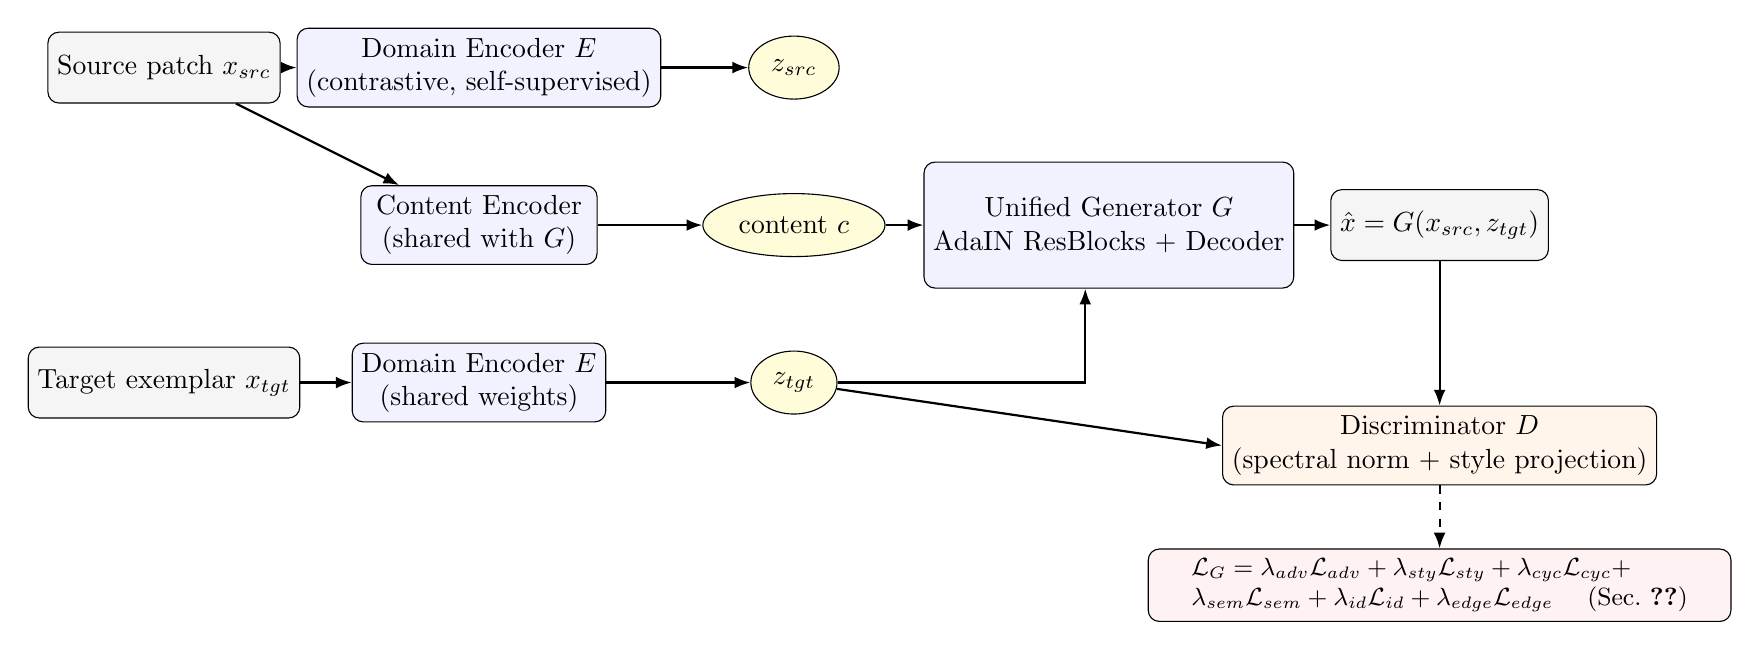
\begin{tikzpicture}[
  node distance=8mm and 10mm,
  box/.style={draw, rounded corners, align=center, minimum height=1.0cm, font=\normalsize, fill=blue!5},
  data/.style={draw, rounded corners, align=center, minimum height=0.9cm, font=\normalsize, fill=gray!8},
  vec/.style={draw, ellipse, align=center, minimum height=0.8cm, font=\normalsize, fill=yellow!15},
  lossbox/.style={draw, rounded corners, align=left, font=\small, fill=red!5},
  arr/.style={-{Latex[length=2mm]}, thick}
]
  \node[data]                              (xsrc) at (0,6)    {Source patch $x_{src}$};
  \node[data]                              (xtgt) at (0,2)    {Target exemplar $x_{tgt}$};

  \node[box, minimum width=3.0cm]          (E1)   at (4.0,6)  {Domain Encoder $E$\\(contrastive, self-supervised)};
  \node[box, minimum width=3.0cm]          (CE)   at (4.0,4)  {Content Encoder\\(shared with $G$)};
  \node[box, minimum width=3.0cm]          (E2)   at (4.0,2)  {Domain Encoder $E$\\(shared weights)};

  \node[vec]                               (zsrc) at (8.0,6)  {$z_{src}$};
  \node[vec]                               (c)    at (8.0,4)  {content $c$};
  \node[vec]                               (ztgt) at (8.0,2)  {$z_{tgt}$};

  \node[box, minimum width=3.2cm, minimum height=1.6cm] (G) at (12.0,4) {Unified Generator $G$\\AdaIN ResBlocks + Decoder};

  \node[data, minimum width=2.6cm]         (xfake) at (16.2,4) {$\hat{x} = G(x_{src}, z_{tgt})$};

  \node[box, fill=orange!8, minimum width=3.0cm] (D) at (16.2,1.2) {Discriminator $D$\\(spectral norm + style projection)};

  \draw[arr] (xsrc) -- (E1);
  \draw[arr] (xsrc) -- (CE);
  \draw[arr] (xtgt) -- (E2);
  \draw[arr] (E1) -- (zsrc);
  \draw[arr] (CE) -- (c);
  \draw[arr] (E2) -- (ztgt);
  \draw[arr] (c) -- (G);
  \draw[arr] (ztgt.east) -| ([xshift=-3mm]G.south);
  \draw[arr] (G) -- (xfake);
  \draw[arr] (xfake) -- (D);
  \draw[arr] (ztgt) -- (D.west);

  \node[lossbox, below=8mm of D, minimum width=7.4cm] (losses) {
    $\mathcal{L}_G = \lambda_{adv}\mathcal{L}_{adv} + \lambda_{sty}\mathcal{L}_{sty} + \lambda_{cyc}\mathcal{L}_{cyc} +$\\
    $\lambda_{sem}\mathcal{L}_{sem} + \lambda_{id}\mathcal{L}_{id} + \lambda_{edge}\mathcal{L}_{edge}$ \quad (Sec.~\ref{sec:objective})
  };
  \draw[arr, dashed] (D.south) -- (losses.north);
\end{tikzpicture}}
\caption{Simplified architecture of the two components reported in this paper: the self-supervised continuous domain encoder $E$ (Objective~1, Sec.~\ref{sec:encoder}) and the unified AdaIN-conditioned generator $G$ with its projection discriminator $D$ (Objective~2, Sec.~\ref{sec:generator}). For clarity, the figure omits two additional forward passes of the source embedding $z_{src}$ through $G$, which are used to compute the cycle-consistency and identity losses of Sec.~\ref{sec:objective}. Components that belong to later objectives of the project (leave-one-pair-out generalization testing and downstream task evaluation) are not shown, because they are outside the scope of this paper.}
\label{fig:architecture}
\end{figure}

Fig.~\ref{fig:architecture} shows the two components covered in this paper. A domain encoder $E$ maps an unlabeled image patch to a continuous style embedding. A content encoder, which is the downsampling path of the generator, extracts a domain-invariant spatial content code. A unified generator $G$ then combines the content of a source patch with the embedding of a target patch to synthesize a translation, which is assessed by a projection discriminator $D$.

\subsection{Self-Supervised Continuous Domain Encoder}
\label{sec:encoder}
The encoder $E_\theta$ receives an $H \times W$ patch with $C$ channels (4 in this implementation: three optical/SAR-derived channels plus one auxiliary channel, see Sec.~\ref{sec:dataset}) and outputs a continuous embedding $z \in \mathbb{R}^{64}$. An input-adapter convolution is followed by three stride-2 convolutional blocks (each Conv--InstanceNorm--LeakyReLU), which progressively reduce the spatial resolution while increasing the channel width. A squeeze-and-excitation (SE) block~\cite{hu2018senet} then recalibrates the channel-wise responses so that the encoder can attend to the most discriminative bands (e.g., near-infrared for vegetation, VV/VH ratio for SAR).

Instead of pooling to a class score, the encoder computes first- and second-order spatial statistics of the final feature map, namely the channel-wise mean $\mu$ and standard deviation $\sigma$. Together, they summarize the radiometric and textural style of the patch independently of its spatial content:
\begin{equation}
\mu_c = \frac{1}{HW}\sum_{i,j} h_{c,i,j}, \qquad
\sigma_c = \sqrt{\frac{1}{HW}\sum_{i,j}(h_{c,i,j}-\mu_c)^2 + \epsilon}
\label{eq:stats}
\end{equation}
where $h$ is the feature map after the SE block. The concatenated statistics $[\mu;\sigma]$ (optionally fused with a projected acquisition-angle feature when angle metadata are available; this option is unused in the sensor-only experiment reported here) pass through a multilayer perceptron projection head and are L2-normalized onto the unit hypersphere:
\begin{equation}
z = \frac{f_\phi([\mu;\sigma])}{\lVert f_\phi([\mu;\sigma]) \rVert_2}, \qquad z \in \mathbb{R}^{64}.
\label{eq:embed}
\end{equation}

The encoder is pretrained without domain labels, using a contrastive pretext task in the style of InfoNCE~\cite{oord2018cpc}. Two independently augmented views ($z_1, z_2$) of the same patch (random flips and 90\textdegree{} rotations) form a positive pair, whereas all other patches in the training batch serve as negatives:
\begin{equation}
\mathcal{L}_{con} = -\frac{1}{2B}\sum_{i=1}^{B}\Big[
\log\frac{e^{\,z_{1,i}\cdot z_{2,i}/\tau}}{\sum_{j} e^{\,z_{1,i}\cdot z_{2,j}/\tau}}
+
\log\frac{e^{\,z_{2,i}\cdot z_{1,i}/\tau}}{\sum_{j} e^{\,z_{2,i}\cdot z_{1,j}/\tau}}
\Big]
\label{eq:infonce}
\end{equation}
where $B$ is the batch size and $\tau$ is a temperature hyperparameter. Since the positive/negative structure comes purely from data augmentation and not from sensor labels, the embedding space is learned without any supervision of domain identity. At inference time, any patch, whether from a domain seen during training or not, can be projected into the same continuous space.

\subsection{Unified Conditional Generator}
\label{sec:generator}
The generator $G_\psi$ receives a source patch $x_{src}$ and a target embedding $z_{tgt}$, which the frozen encoder $E$ produces from a target-domain exemplar, and it synthesizes a translated patch $\hat{x} = G_\psi(x_{src}, z_{tgt})$. One generator instance is shared across all domains, and the target style is determined entirely by $z_{tgt}$. Translation into any domain that the encoder can embed, and not only the domains enumerated at training time, therefore requires neither architectural changes nor additional parameters.

The content path follows an encoder-bottleneck-decoder design in the spirit of StarGAN~v2~\cite{choi2020starganv2}, adapted to be label-free. A content encoder with reflection-padded convolutions and instance normalization downsamples $x_{src}$ into a domain-invariant content code $c = \mathrm{Enc}_c(x_{src})$. This code passes through four residual blocks modulated by Adaptive Instance Normalization (AdaIN)~\cite{huang2017adain}, which injects the target style at every block:
\begin{equation}
\mathrm{AdaIN}(h, z) = \gamma(z)\cdot\frac{h - \mu(h)}{\sigma(h)} + \beta(z)
\label{eq:adain}
\end{equation}
where $\mu(h), \sigma(h)$ are the per-channel instance statistics of the intermediate feature map $h$, and $\gamma(z) = W_\gamma z + b_\gamma$, $\beta(z) = W_\beta z + b_\beta$ are affine parameters regressed from the continuous embedding. The decoder mirrors the encoder with two AdaIN-modulated upsampling stages. It uses bilinear upsampling, instead of nearest-neighbor or transposed-convolution upsampling, to avoid checkerboard artifacts, and it ends with a reflection-padded output convolution with a $\tanh$ activation.

\subsection{Discriminator with Continuous Style Projection}
The discriminator $D_\xi$ is a multi-scale PatchGAN in which spectral normalization~\cite{miyato2018spectral} is applied to every convolutional layer; this stabilizes adversarial training by bounding the Lipschitz constant of each layer. Besides an unconditional real/fake head, $D_\xi$ projects its intermediate features onto the conditioning embedding $z$:
\begin{equation}
D_\xi(x, z) = D_{uncond}(x) + \frac{\langle \phi(x), W_{proj}\,z\rangle}{\sqrt{d}}
\label{eq:disc}
\end{equation}
where $\phi(x)$ is the penultimate feature map of the discriminator, $W_{proj}$ is a learned linear projection of the embedding, and $d$ is the feature dimension. This term penalizes translations whose visual style does not match the conditioning embedding $z$, and it thereby complements the style-reconstruction signal obtained from the encoder (Sec.~\ref{sec:objective}).

\subsection{Composite Training Objective}
\label{sec:objective}
The generator is trained with a weighted sum of six loss terms. Each term targets a specific failure mode observed in unconstrained multi-domain translation.

\emph{Adversarial loss} (least-squares GAN~\cite{mao2017lsgan}), which encourages $\hat{x}$ to be indistinguishable from real target-domain patches under the style-conditioned discriminator:
\begin{align}
\mathcal{L}_D &= \tfrac{1}{2}\mathbb{E}\big[(D_\xi(x_{tgt}, z_{tgt}) - 1)^2\big] + \tfrac{1}{2}\mathbb{E}\big[D_\xi(\hat{x}, z_{tgt})^2\big] \\
\mathcal{L}_{adv} &= \mathbb{E}\big[(D_\xi(\hat{x}, z_{tgt}) - 1)^2\big]
\label{eq:adv}
\end{align}

\emph{Style-reconstruction loss}, which requires that the target style can be measured in the output by re-encoding it:
\begin{equation}
\mathcal{L}_{sty} = \mathbb{E}\,\lVert E(\hat{x}) - z_{tgt} \rVert_1
\label{eq:sty}
\end{equation}

\emph{Cycle-consistency loss}~\cite{zhu2017cyclegan}, which translates $\hat{x}$ back toward the source style and requires the original patch to be recovered, thereby discouraging mode collapse across domains:
\begin{equation}
\mathcal{L}_{cyc} = \mathbb{E}\,\lVert G(\hat{x}, z_{src}) - x_{src} \rVert_1
\label{eq:cyc}
\end{equation}

\emph{Semantic-preservation loss}, which penalizes drift of the domain-invariant content code between the source and the translation, so that the geospatial layout (parcel boundaries, roads) is not altered by the style change:
\begin{equation}
\mathcal{L}_{sem} = \mathbb{E}\,\lVert \mathrm{Enc}_c(\hat{x}) - \mathrm{Enc}_c(x_{src}) \rVert_1
\label{eq:sem}
\end{equation}

\emph{Identity loss}, which requires that conditioning the generator on the source's own style leaves the patch unchanged:
\begin{equation}
\mathcal{L}_{id} = \mathbb{E}\,\lVert G(x_{src}, z_{src}) - x_{src} \rVert_1
\label{eq:id}
\end{equation}

\emph{Edge-preservation loss}, which compares the Sobel gradient magnitudes of $\hat{x}$ and $x_{src}$ in order to keep agricultural parcel boundaries and road edges sharp:
\begin{equation}
\mathcal{L}_{edge} = \mathbb{E}\,\lVert \nabla_{Sobel}(\hat{x}) - \nabla_{Sobel}(x_{src}) \rVert_1
\label{eq:edge}
\end{equation}

The total generator objective is
\begin{align}
\mathcal{L}_G ={}& \lambda_{adv}\mathcal{L}_{adv} + \lambda_{sty}\mathcal{L}_{sty} + \lambda_{cyc}\mathcal{L}_{cyc} \notag \\
& + \lambda_{sem}\mathcal{L}_{sem} + \lambda_{id}\mathcal{L}_{id} + \lambda_{edge}\mathcal{L}_{edge}
\label{eq:total}
\end{align}
with the weights listed in Table~\ref{tab:hyperparams}. In addition, the framework defines a geometric (SSIM-style) preservation loss $\mathcal{L}_{geo}$, which is activated when the source or the target domain is an off-nadir viewing-angle domain. The PASTIS-HD experiment reported in Sec.~\ref{sec:results} uses only sensor domains, so $\mathcal{L}_{geo}$ is inactive ($\lambda_{geo}\mathcal{L}_{geo}=0$) for the results presented here.

\section{Dataset and Preprocessing}
\label{sec:dataset}
The experiments use patches derived from PASTIS-HD~\cite{garnot2021panoptic,astruc2024omnisat}, a real and publicly released benchmark of $2{,}433$ co-registered agricultural-parcel locations across metropolitan France. Each location is available as a Sentinel-2 optical time series, a Sentinel-1 SAR time series, and, in the HD extension, a very-high-resolution SPOT~6/7 image. A conversion pipeline in the accompanying codebase matches patches across modalities by their shared patch identifier and exports one $128\times128$, 4-channel tensor per modality and location. For Sentinel-2, only the Red, Green, Blue, and near-infrared bands of a single temporal acquisition are kept. The SPOT~6/7 imagery is resized from its native $1280\times1280$ resolution to $128\times128$ and supplemented with a synthetic near-infrared proxy channel. The VV and VH polarizations of Sentinel-1 SAR are extended with a derived ratio channel and an average channel, and are normalized from decibel units. All modalities are scaled to $[-1,1]$. Of the up to $2{,}433$ available locations, this experiment converts $1{,}500$ per domain, a number limited by the patch cap of the conversion pipeline (Table~\ref{tab:dataset}). The converted patches are the first $1{,}500$ in identifier order and originate from three Sentinel-2 tiles. An 80/20 split by identifier order yields $1{,}200$ training patches and $300$ held-out patches per domain. As a consequence, all held-out patches belong to a single tile (T31TFM) that is only marginally represented in the training data, so the held-out evaluation is largely a test on a different region. The modalities are co-registered but not simultaneous: the first Sentinel-1 acquisition follows the first Sentinel-2 acquisition by 11~days at the median, and the SPOT imagery dates from 2019, whereas the Sentinel data begin in September 2018. After conversion, the SAR difference channel is saturated at $+1$ for 97.9\% of its values. Training-split patches are augmented on the fly with random horizontal and vertical flips, random 90\textdegree{} rotations, and small per-channel Gaussian radiometric noise ($\sigma \sim \mathcal{U}[0, 0.01]$).

\begin{table}[t]
\centering
\caption{Converted PASTIS-HD patches used in this study.}
\label{tab:dataset}
\begin{tabular}{@{}lccc@{}}
\toprule
\textbf{Domain} & \textbf{Modality} & \textbf{Channels} & \textbf{Patches} \\
\midrule
Sentinel-2       & Multispectral optical (R,G,B,NIR) & 4 & 1{,}500 \\
SPOT 6/7         & VHR optical (+NIR proxy)          & 4 & 1{,}500 \\
Sentinel-1 SAR   & C-band radar (VV, VH, ratio, avg) & 4 & 1{,}500 \\
\bottomrule
\end{tabular}
\end{table}

\section{Experimental Setup}
\label{sec:setup}
The framework is implemented in Python~3.13 with PyTorch~$\geq$2.4; NumPy, SciPy, Pillow, Matplotlib, and PyYAML are used for data handling, preprocessing, and visualization. A single command-line entry point orchestrates training: it first runs domain-encoder pretraining and then trains the generator and discriminator jointly. All training and evaluation were run on the CPU of a laptop (Intel Core i7-9750H, 6 cores, 7.8~GB RAM, Windows~11) with a CPU-only PyTorch build. The channel width of the generator and discriminator was deliberately kept narrow (base width 32) so that training remains tractable at this compute scale, and not in order to match a specific reported baseline configuration. Table~\ref{tab:hyperparams} lists the hyperparameters used for the results in Sec.~\ref{sec:results}.

\begin{table}[t]
\centering
\caption{Training hyperparameters.}
\label{tab:hyperparams}
\begin{tabular}{@{}ll@{}}
\toprule
\textbf{Stage 1 -- Domain Encoder} & \textbf{Value} \\
\midrule
Embedding dimension $d$            & 64 \\
Optimizer                          & AdamW \\
Learning rate                      & $5\times10^{-4}$ \\
Weight decay                       & $1\times10^{-4}$ \\
Contrastive temperature $\tau$     & 0.07 \\
Epochs                             & 10 \\
\midrule
\textbf{Stage 2 -- Generator / Discriminator} & \textbf{Value} \\
\midrule
Base channel width                 & 32 \\
Residual blocks                    & 4 \\
Optimizer ($G$, $D$)               & Adam ($\beta_1{=}0.5$, $\beta_2{=}0.999$) \\
Learning rate ($G$, $D$)           & $3\times10^{-4}$ \\
LR schedule                        & Cosine annealing, $\eta_{min}{=}10^{-5}$ \\
Gradient clipping (max norm)       & 1.0 \\
Epochs                             & 12 \\
Batch size                         & 8 \\
$\lambda_{adv},\lambda_{sty},\lambda_{id}$ & 1.0 each \\
$\lambda_{sem}$, $\lambda_{edge}$  & 2.0 each \\
$\lambda_{cyc}$                    & 10.0 \\
\bottomrule
\end{tabular}
\end{table}

\section{Results and Discussion}
\label{sec:results}
All results were measured on the 300 held-out patches per domain with a fixed protocol, and each is a single measurement of one trained model. The style of a target domain is defined as the L2-normalized mean of the embeddings of its 1{,}200 training patches (the domain \emph{centroid}); domain labels and co-registered patches are used only for evaluation. Image metrics are computed on images rescaled to $[0,1]$ against the co-registered real target patch, and two reference baselines are included: the untranslated source patch (``Copy'') and a constant image equal to the mean of the target domain (``Const.'').

\subsection{Domain encoder (Objective~1)}
Table~\ref{tab:enc} summarizes the results for the encoder. It solves its contrastive task on held-out patches (loss 0.24, against 2.08 for an uninformative embedding; 88.2\% top-1 retrieval of the second view among 900 patches), and its embeddings are distributed continuously over the hypersphere and do not form three tight clusters. However, they describe the sensor only moderately well: the nearest centroid assigns 65.8\% of the held-out patches to the correct sensor, against 33.3\% by chance; the sensors overlap (silhouette coefficient 0.11); and the effective dimensionality is about four. Retrieval of the co-registered patch from another sensor is at chance level, which indicates that the embedding does not carry scene content shared across sensors. A likely explanation, which was not tested, is that instance discrimination rewards distinguishing individual patches and includes no term that groups the patches of one sensor; the proximity-based positive pairs foreseen in the project plan were not used.

\begin{table}[t]
\centering
\caption{Domain encoder evaluated on 300 held-out patches per domain (S2: Sentinel-2).}
\label{tab:enc}
\begin{tabular}{@{}lc@{}}
\toprule
\textbf{Measurement} & \textbf{Result} \\
\midrule
Held-out InfoNCE loss (batch 8; chance 2.08)        & 0.24 \\
Top-1 instance retrieval among 900 patches          & 88.2\% \\
Nearest-centroid domain accuracy (chance 33.3\%)    & 65.8\% \\
\quad recall S2 / SPOT / SAR                        & 62.7 / 74.3 / 60.3\% \\
5-nearest-neighbor domain accuracy                  & 63.7\% \\
Cosine similarity within / between domains          & 0.32 / 0.04 \\
Silhouette coefficient (cosine distance)            & 0.11 \\
Participation ratio (of 64 dimensions)              & 3.85 \\
Same-location retrieval across sensors, top-1       & 0.3\% (chance 0.3\%) \\
\bottomrule
\end{tabular}
\end{table}

\subsection{Conditional generator (Objective~2)}
\begin{figure}[t]
\centering
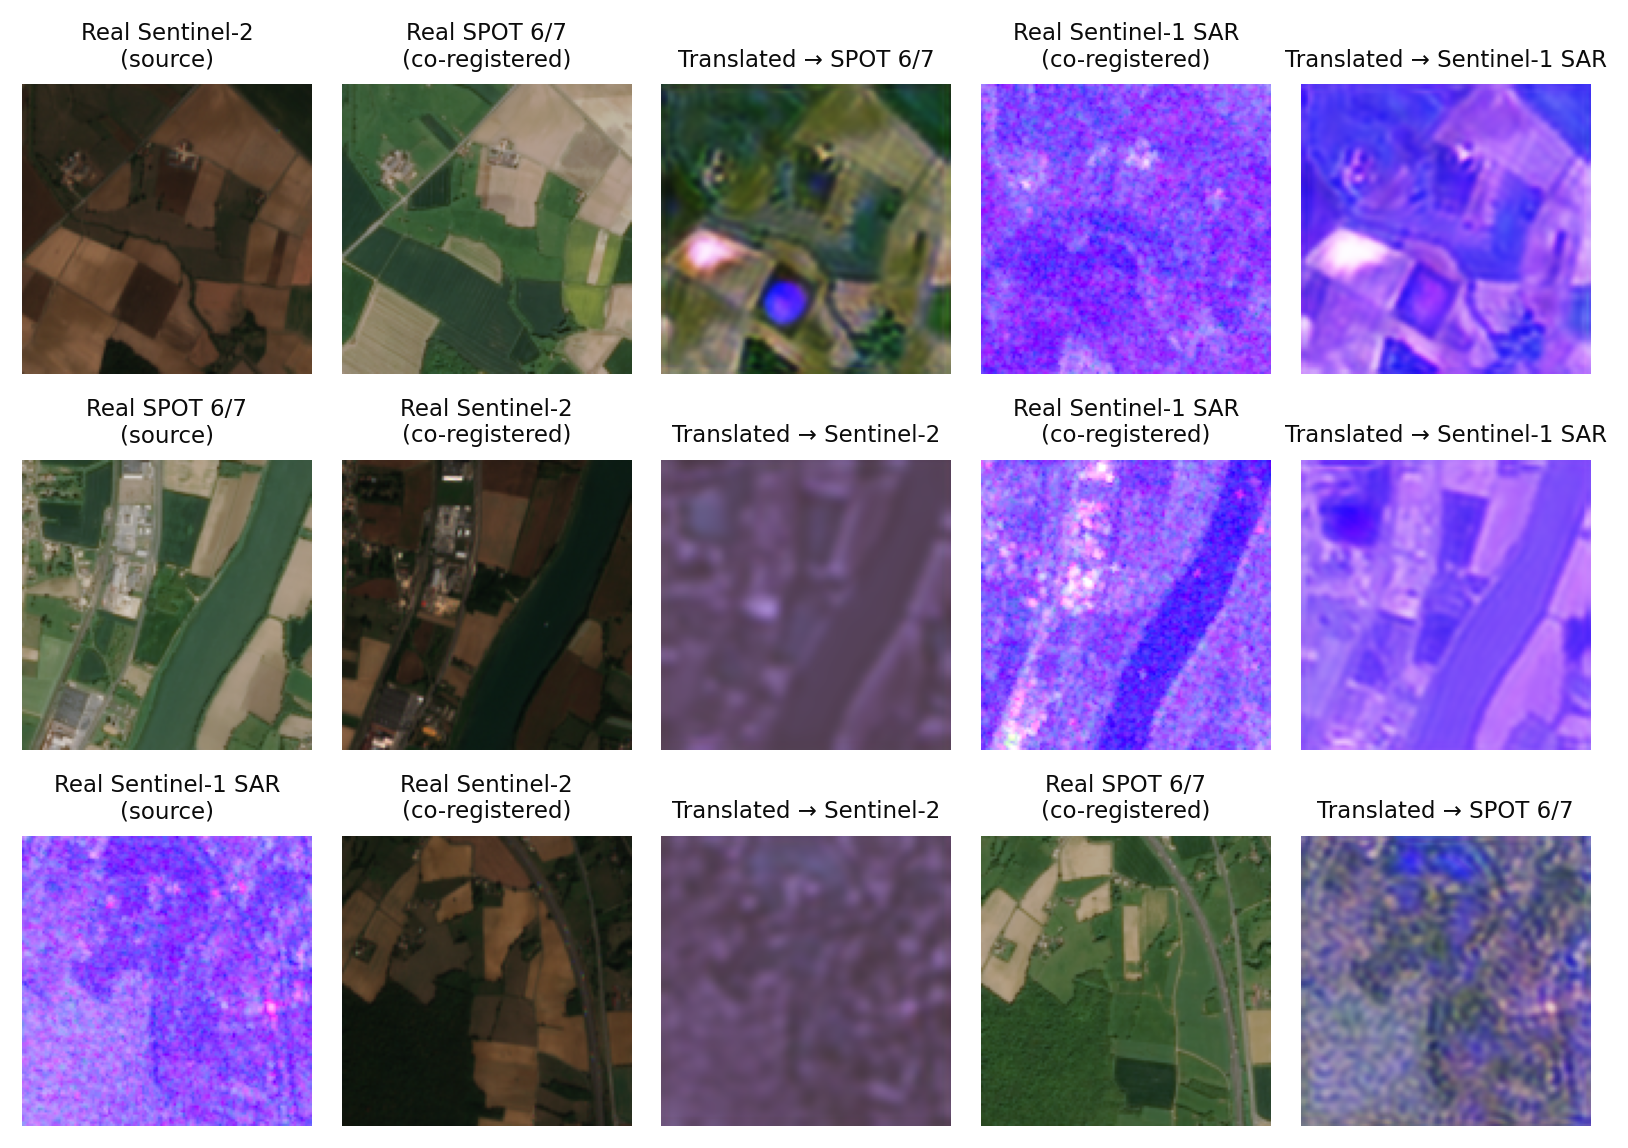
\includegraphics[width=\textwidth]{figures/fig_paired_translation.png}
\caption{Translations of one held-out patch per source domain (first column of each row) into the two other domains, shown next to the real co-registered patch of each target domain. The style is the centroid embedding of the target domain, and the patches were selected with a fixed random seed before inspection. Sentinel-1 patches are displayed with VV, VH, and the saturated difference channel as the red, green, and blue channels, respectively.}
\label{fig:paired}
\end{figure}

\begin{table}[t]
\centering
\caption{Translation into each target domain on held-out patches. PSNR (dB) against the co-registered real target patch is given for the translation, for the copied source (Copy), and for a constant target-mean image (Const.). Style is the share of outputs that the encoder assigns to the target domain, and Edge is the edge-map correlation with the source.}
\label{tab:gen}
\footnotesize
\setlength{\tabcolsep}{3.5pt}
\begin{tabular}{@{}lccccc@{}}
\toprule
\textbf{Pair} & \textbf{Transl.} & \textbf{Copy} & \textbf{Const.} & \textbf{Style} & \textbf{Edge} \\
\midrule
S2 $\rightarrow$ SPOT   & 14.6 & 13.1 & 17.2 & 57\% & 0.82 \\
S2 $\rightarrow$ SAR    & 14.6 & 5.7 & 20.5 & 18\% & 0.87 \\
SPOT $\rightarrow$ S2   & 13.5 & 13.1 & 17.8 & 29\% & 0.71 \\
SPOT $\rightarrow$ SAR  & 16.8 & 7.4 & 20.5 & 80\% & 0.82 \\
SAR $\rightarrow$ S2    & 13.3 & 5.7 & 17.8 & 12\% & 0.94 \\
SAR $\rightarrow$ SPOT  & 13.0 & 7.4 & 17.2 & 45\% & 0.92 \\
\bottomrule
\end{tabular}
\end{table}

Fig.~\ref{fig:paired} and Table~\ref{tab:gen} summarize the results for the generator. \emph{Structure is preserved:} the edge-map correlation between the source and the output ranges from 0.71 to 0.94, which is higher than the 0.61 to 0.70 observed between real patches of different sensors, and parcels, the river, and the road remain recognizable in the figure. \emph{The style vector is used:} with the correct target style, the PSNR is higher than with the style of the third domain for five of the six pairs (by 3.3 to 7.6~dB), and the translation is better than copying the source for all six pairs, most strongly for the pairs that involve SAR. \emph{Target radiometry is not reproduced:} for all six pairs, a constant image equal to the target-domain mean agrees better with the real target patch than the translation does (by 2.6 to 5.9~dB). In addition, the encoder assigns the outputs to the target domain in only 12\% to 80\% of the cases. Translations into Sentinel-2 appear as a blurred purple-gray haze whose channel means are identical for all three sources (within 0.001) and much brighter than those of real Sentinel-2 patches (by 0.59 in the blue channel on a $[-1,1]$ scale). The identity mapping of Sentinel-2 is also poorly reproduced (13.7~dB, compared with 20.3~dB for SPOT and 24.3~dB for SAR), which makes Sentinel-2 the weak point of the generator both as a source and as a target. Differences in acquisition date between the modalities limit the achievable pixel agreement, but they do not explain why the translation is worse than a constant image.

\emph{Continuity of the style space} was examined by interpolating between two domain centroids, $z(\alpha)=(1-\alpha)\bar z_a+\alpha\bar z_b$, renormalized to unit length, for 300 source patches. For the two pairs that involve SAR, the output changes smoothly and almost linearly (linearity ratio 0.91 and 0.96; monotone for 96\% and 100\% of the patches). For Sentinel-2 and SPOT, the change is about half as large, is concentrated in the first step from $\alpha=0$ to $\alpha=0.25$, and is monotone for only 41\% of the patches. The generator has 1.59~M parameters and the encoder 0.89~M, and one translation takes about 84~ms per patch on the CPU. Fig.~\ref{fig:interp} illustrates this interpolation for one held-out SPOT~6/7 source patch.

\begin{figure}[t]
\centering
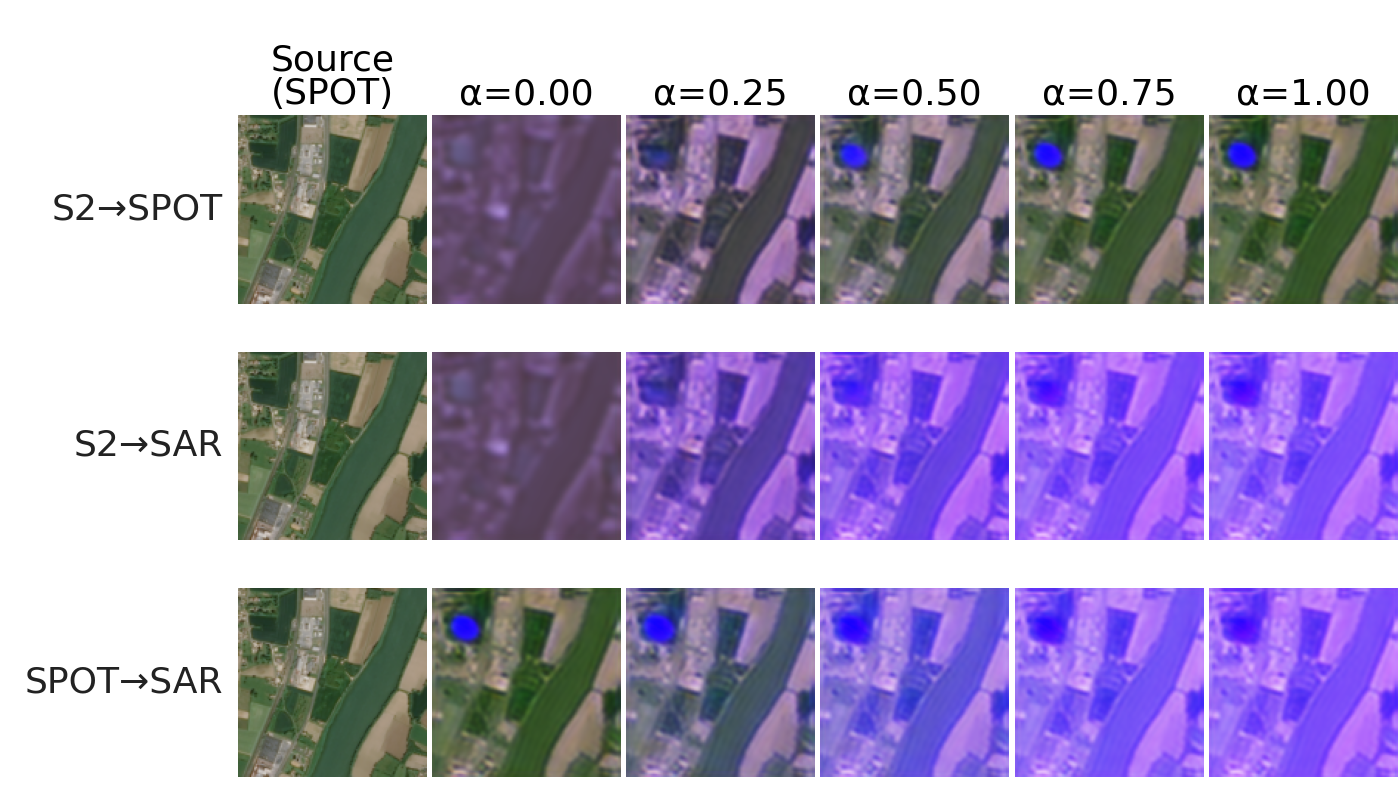
\includegraphics[width=0.85\textwidth]{figures/fig_interp_compact.png}
\caption{Interpolation of the style vector between two domain centroids, $z(\alpha)=(1-\alpha)\bar z_a+\alpha\bar z_b$, renormalized to unit length, applied to one held-out SPOT~6/7 source patch (first column). Each row corresponds to a domain pair $a \rightarrow b$, and $\alpha$ runs from the style of $a$ ($\alpha=0$) to the style of $b$ ($\alpha=1$). The patch was selected with a fixed random seed before inspection.}
\label{fig:interp}
\end{figure}

\section{Comparative Analysis}
Table~\ref{tab:gap} in Sec.~\ref{sec:gap} has already placed the proposed encoder-generator pair alongside the closest prior methods with respect to the properties that motivate this work. In the implementation, the design goals listed in Table~\ref{tab:gap} are met at the architectural level: training uses no domain labels, one generator serves all ordered pairs of three domains, and the domain code is a continuous 64-dimensional embedding. The quality of the results, however, cannot be compared with the cited methods, because none of them was trained on the same data and their published figures come from other datasets and tasks. Accordingly, no claim is made that the approach outperforms SS(DA)$^2$, StarGAN~v2, or the other methods.

\section{Limitations}
\label{sec:limitations}
Several limitations should be kept in mind when interpreting the results in Sec.~\ref{sec:results}. First, the held-out patches come from a single Sentinel-2 tile, whereas the training set is dominated by two other tiles; the results therefore combine model quality with a region shift, and in particular the domain centroids come from mostly different regions than the patches to which they are applied. Second, the modalities are not simultaneous, which limits pixel-level agreement with the co-registered reference, and the preprocessing introduces artifacts (a saturated SAR channel and a synthetic fourth SPOT channel). Third, each model was trained only once, with a short schedule (10 encoder and 12 generator epochs), a narrow network (base width 32), and a CPU-only laptop (Sec.~\ref{sec:setup}). The training loops are not seeded, the run-to-run variation is unknown, no ablation of the six generator losses was run, and no other translation method was trained on the same data for comparison. Fourth, PSNR and SSIM measure agreement with a co-registered image and not realism, and the style-transfer success rate is judged by the same encoder that conditions the generator, so it is only as reliable as that encoder. Fifth, only three sensor domains, one geographic setting, and $1{,}500$ of the $2{,}433$ locations are used; the larger MSC-France corpus foreseen for encoder pretraining was not used, and the angle-domain conditioning implemented in the framework was not exercised. Finally, generalization to unseen sensor pairs and downstream accuracy (Objectives~3--4) were not evaluated.

\section{Conclusion and Future Work}
This paper presented the first two components of a self-supervised, multi-domain adaptation framework for satellite imagery. The first is a contrastive domain encoder that learns continuous, label-free embeddings of sensor style from unlabeled multi-sensor patches. The second is a unified AdaIN-conditioned generator that uses this embedding, in place of the discrete domain labels required by prior multi-domain translators, to translate the content of a source patch into an arbitrary target style. Implemented and trained on real PASTIS-HD imagery across Sentinel-2, SPOT~6/7, and Sentinel-1 SAR, the framework meets its design goals at the architectural level: no domain labels, one model for all ordered domain pairs, and a continuous domain code. The measured quality is limited, however. The encoder identifies the sensor only moderately (65.8\% against 33.3\% by chance), and the generator preserves scene structure and uses the style vector but does not reproduce the radiometry of the target sensor, while translations into Sentinel-2 fail.

Building directly on these findings, future work will (i) replace the augmented-view positives of the encoder with sensor-aware positive pairs based on spatial and temporal proximity, and pretrain on the larger MSC-France corpus; (ii) correct the data issues identified here by using all PASTIS-HD patches with a tile-stratified split, temporally matched acquisitions, and a non-saturating SAR channel; (iii) train wider networks for longer on a GPU, with seeded and logged runs, loss ablations, and baselines trained on the same data; and (iv) carry out the leave-one-domain-pair-out and zero-shot (SpaceNet~6) generalization evaluation, together with the downstream crop-classification and segmentation evaluation, which constitute Objectives~3 and~4 of the broader project.

\bibliographystyle{splncs04}
\bibliography{references}

\end{document}
"
\ifdefined\ANON
\author{Anonymous Authors}
\authorrunning{Anonymous Authors}
\institute{Anonymous Institution}
\else
\author{Shivangi\textsuperscript{1} \and Benedict Tephila M.\textsuperscript{2} \and Naveen J.\textsuperscript{3}}
\authorrunning{S. et al.}
\institute{Department of Computer Science and Engineering,\\
CHRIST (Deemed to be University), Bangalore -- 560029, India\\
\textsuperscript{1}\email{shivangi.a@mtech.christuniversity.in},
\textsuperscript{2}\email{benedict.tephila@christuniversity.in},
\textsuperscript{3}\email{naveen.j@christuniversity.in}}
\fi

\maketitle

\begin{abstract}
Deep learning models for satellite image analysis are usually trained on imagery from a particular sensor, season, or geographic region, and their performance is known to deteriorate when the same land-cover classes are observed under a different acquisition domain. Current domain-adaptation approaches for satellite imagery generally depend on labeled target-domain data, on a discrete predefined set of domains, or on both. Such assumptions are hard to meet in practice, particularly for growing multi-sensor archives in which domain boundaries are not always clearly defined. This paper reports the first two components of a broader self-supervised multi-domain adaptation framework for satellite imagery. The first is (i) a continuous domain encoder that learns a label-free, continuous-valued style embedding directly from unlabeled multi-sensor image patches by means of a contrastive (InfoNCE) pretext task. The second is (ii) a unified conditional generator that translates the content of a source-domain patch into the style of an arbitrary target domain with a single Adaptive Instance Normalization (AdaIN)-modulated network, which is conditioned on the continuous embedding instead of a discrete domain label. Both networks were trained on a CPU using 1{,}200 patches per sensor from the real PASTIS-HD benchmark (Sentinel-2, SPOT~6/7, and Sentinel-1 SAR) and were evaluated on 300 held-out patches per sensor drawn from a largely different region. The encoder solves its pretext task, but it identifies the sensor only moderately well (65.8\% against 33.3\% by chance). The generator preserves scene structure and responds smoothly to interpolated styles for the pairs that involve SAR; however, it does not reproduce the radiometry of the target sensor. A constant image agrees better with the real target patch than the translation does, and translations into Sentinel-2 collapse to a source-independent color cast. Generalization to unseen sensor pairs and downstream accuracy lie outside the scope of this paper.
\keywords{domain adaptation \and self-supervised learning \and generative adversarial networks \and contrastive learning \and multi-sensor satellite imagery \and image-to-image translation}
\end{abstract}


\section{Introduction}

Satellite remote sensing has shifted from single-mission analysis to a setting in which optical and radar constellations -- Sentinel-2, Landsat, SPOT, and a growing set of commercial very-high-resolution (VHR) and synthetic aperture radar (SAR) platforms -- image the Earth's surface jointly and continuously. Deep learning models for land-cover classification, crop mapping, and change detection are therefore increasingly expected to operate across this heterogeneous, multi-sensor archive rather than only on the sensor on which they were trained.

Meeting this cross-sensor requirement is difficult in practice. Every sensor has its own radiometric calibration, spectral response, spatial resolution, and noise characteristics, and the resulting effects range from atmospheric haze and calibration drift in optical imagery to speckle noise and incidence-angle-dependent backscatter in SAR. Consequently, a model trained on the statistics of one sensor can lose a great deal of accuracy when it is applied to another sensor, even if the underlying land-cover classes are identical. Because acquiring and annotating imagery from every sensor of interest is costly, models often have to be adapted to a new domain with little or no labeled target-domain data.

Existing approaches to this problem fall broadly into two families. Domain-adaptation methods designed specifically for satellite imagery, such as multi-source standardization~\cite{tasar2020standardgan}, condition the translation on a discrete, manually assigned domain identity and have been shown to struggle with domain-pair combinations that were not seen during training. Self-supervised alternatives such as SS(DA)$^2$~\cite{zhang2023ssdada} need neither labels nor an explicit domain boundary, but they are formulated for translation between exactly two satellites at a time, so every new sensor pair requires separate training. In the wider image-to-image translation literature, StarGAN~\cite{choi2018stargan} and StarGAN~v2~\cite{choi2020starganv2} unify translation across many domains in a single generator, and StarGAN~v2 replaces discrete domain labels with a learned continuous style code. Both, however, are trained with supervised, discretely indexed domain labels, and they are evaluated on natural-image benchmarks (faces, animal faces) with visual-realism metrics, rather than on satellite imagery or on downstream task correctness. More recent diffusion-based translators~\cite{vinholi2024multisensor,kieu2025universal} improve translation quality, and the diffusion router~\cite{kieu2025universal} additionally routes between multiple domains. Nevertheless, these methods still operate over a discrete, pre-enumerated set of domains and incur the considerably higher inference cost of iterative diffusion sampling.

In summary, the literature does not yet provide a method that combines, for satellite imagery, three properties at once: label-free training, a continuous representation of the domain (rather than a fixed-cardinality, discretely labeled one), and a single generator capable of translating into an arbitrary target style. This gap motivates the present work.

We address the first two of these properties by carrying the self-supervised, label-free philosophy of SS(DA)$^2$ over from a pairwise setting to a continuous, StarGAN~v2-style unified generator that does not require discrete domain conditioning. Specifically, a contrastive domain encoder is pretrained on unlabeled multi-sensor patches to produce a continuous embedding of each patch's sensor/style characteristics. A single conditional generator, modulated through AdaIN by this embedding, then translates a source patch into the style of any target patch's embedding, including domain combinations that were not explicitly indexed during training. This paper reports the design, implementation, and held-out evaluation of these two components. The remaining objectives of the broader project, namely generalization testing on unseen sensor-pair combinations and downstream task evaluation, are implemented in the accompanying codebase but fall outside the scope of this paper.

The contributions of this paper are:
\begin{itemize}
\item A self-supervised contrastive domain encoder that yields continuous, label-free embeddings of sensor/style characteristics directly from unlabeled multi-sensor satellite patches.
\item A single, unified AdaIN-modulated conditional generator that is conditioned on this continuous embedding instead of a discrete domain code, which makes translation into an arbitrary target style possible without retraining for each domain pair.
\item A composite training objective that combines adversarial, style-reconstruction, cycle-consistency, semantic-preservation, identity, and edge-preservation losses and is designed to keep geospatial content intact while the sensor-specific style is changed.
\item An implementation and held-out evaluation on the real PASTIS-HD multi-sensor benchmark (Sentinel-2, SPOT~6/7, Sentinel-1~SAR) that reports both what the approach achieves (label-free continuous embeddings, structure-preserving and style-conditioned translation) and where it falls short (moderate sensor information in the embedding, target radiometry not reproduced).
\end{itemize}

\section{Related Work}

\subsection{Domain Adaptation for Satellite Imagery}
StandardGAN~\cite{tasar2020standardgan} tackles multi-source domain adaptation for semantic segmentation of VHR satellite images. It standardizes the data distribution of each source domain toward a common reference before downstream training. The method operates over a discrete, enumerated set of source domains and, according to its authors, has difficulty preserving image content faithfully and generalizing to sensor combinations that were not standardized against directly. SS(DA)$^2$~\cite{zhang2023ssdada}, the base paper on which the present framework builds, eliminates the need for labeled target data and an explicit domain boundary: it trains a contrastive, domain-agnostic GAN that translates between two satellite domains using only unlabeled imagery. Its central limitation, and the specific gap addressed in this paper, is that the formulation is pairwise. Each trained model supports exactly two satellites, so adding a new sensor to the archive requires an additional model.

\subsection{Multi-Domain Image-to-Image Translation}
StarGAN~\cite{choi2018stargan} was the first method to unify multi-domain translation in a single generator; it conditions the network on a discrete one-hot domain vector provided at both training and inference time. StarGAN~v2~\cite{choi2020starganv2} replaces this discrete label with a continuous style code, which is produced by a mapping network or a style encoder and injected into the generator through AdaIN~\cite{huang2017adain}; its authors report substantially more diverse and realistic synthesis. Both methods, however, are trained with supervised domain labels and are evaluated on natural-image datasets (human/animal faces) with visual-realism metrics (e.g., FID), rather than on satellite imagery or with a task-grounded correctness metric. Diffusion-based translators have since been proposed for multi-sensor optical imagery~\cite{vinholi2024multisensor} and for universal multi-domain routing~\cite{kieu2025universal}. Although they improve sample fidelity, the router in~\cite{kieu2025universal} still selects among a discrete, pre-specified set of domain experts, and diffusion sampling is computationally more expensive at inference than a single feed-forward GAN pass, which is relevant when large satellite mosaics are translated.

\section{Research Gap and Motivation}
\label{sec:gap}
Table~\ref{tab:gap} compares the properties of the most closely related methods with those targeted by this work. None of the prior methods reviewed here combines label-free training with a continuous (open-ended) domain representation in a single generator that is designed for, and evaluated on, satellite imagery. SS(DA)$^2$ provides the first property but not the second, since it is pairwise only. StarGAN~v2 provides the second but not the first, because it needs supervised discrete labels at training time, and it is neither designed for nor evaluated on remote-sensing data. StandardGAN targets satellite imagery but requires a discrete domain identity. Objectives~1 and~2 of the present project, a label-free continuous domain encoder and a single unified generator conditioned on that continuous embedding, are intended to close this particular combination of gaps. Objectives~3 and~4 (generalization to unseen domain-pair combinations and downstream task evaluation) build on this foundation but are outside the scope of this paper.

\begin{table}[t]
\centering
\caption{Qualitative comparison of the properties relevant to the identified research gap.}
\label{tab:gap}
\resizebox{\linewidth}{!}{%
\begin{tabular}{@{}lccc@{}}
\toprule
\textbf{Method} & \textbf{Label-free} & \textbf{Continuous domain repr.} & \textbf{Satellite-specific} \\
\midrule
StandardGAN~\cite{tasar2020standardgan}    & \ding{55} & \ding{55} & \ding{51} \\
SS(DA)$^2$~\cite{zhang2023ssdada}          & \ding{51} & \ding{55} (pairwise) & \ding{51} \\
StarGAN~\cite{choi2018stargan}             & \ding{55} & \ding{55} & \ding{55} \\
StarGAN~v2~\cite{choi2020starganv2}        & \ding{55} & \ding{51} & \ding{55} \\
\textbf{Proposed (Objectives 1--2)}        & \ding{51} & \ding{51} & \ding{51} \\
\bottomrule
\end{tabular}}
\end{table}

\section{Proposed Methodology}

\begin{figure}[t]
\centering
\resizebox{\textwidth}{!}{%
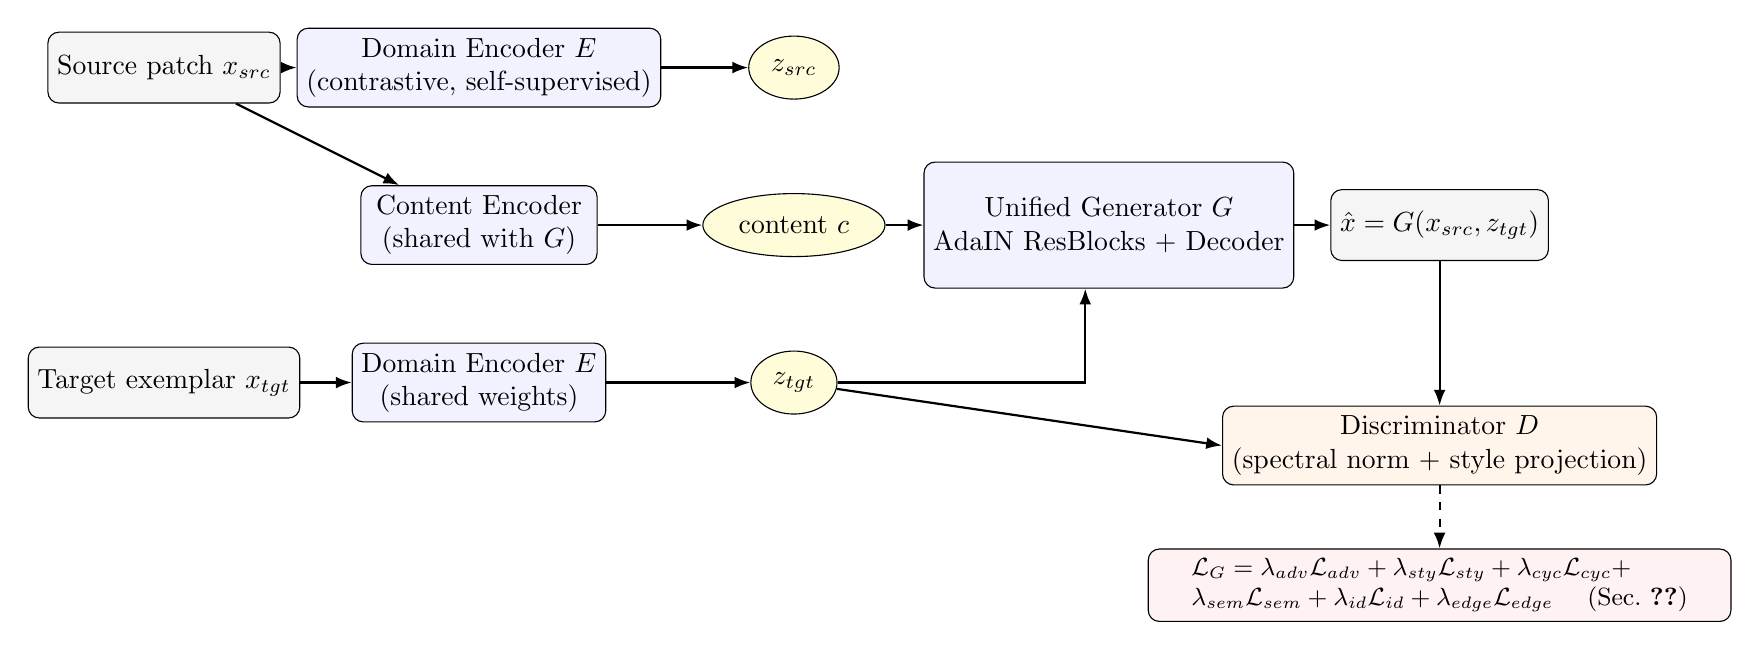
\begin{tikzpicture}[
  node distance=8mm and 10mm,
  box/.style={draw, rounded corners, align=center, minimum height=1.0cm, font=\normalsize, fill=blue!5},
  data/.style={draw, rounded corners, align=center, minimum height=0.9cm, font=\normalsize, fill=gray!8},
  vec/.style={draw, ellipse, align=center, minimum height=0.8cm, font=\normalsize, fill=yellow!15},
  lossbox/.style={draw, rounded corners, align=left, font=\small, fill=red!5},
  arr/.style={-{Latex[length=2mm]}, thick}
]
  \node[data]                              (xsrc) at (0,6)    {Source patch $x_{src}$};
  \node[data]                              (xtgt) at (0,2)    {Target exemplar $x_{tgt}$};

  \node[box, minimum width=3.0cm]          (E1)   at (4.0,6)  {Domain Encoder $E$\\(contrastive, self-supervised)};
  \node[box, minimum width=3.0cm]          (CE)   at (4.0,4)  {Content Encoder\\(shared with $G$)};
  \node[box, minimum width=3.0cm]          (E2)   at (4.0,2)  {Domain Encoder $E$\\(shared weights)};

  \node[vec]                               (zsrc) at (8.0,6)  {$z_{src}$};
  \node[vec]                               (c)    at (8.0,4)  {content $c$};
  \node[vec]                               (ztgt) at (8.0,2)  {$z_{tgt}$};

  \node[box, minimum width=3.2cm, minimum height=1.6cm] (G) at (12.0,4) {Unified Generator $G$\\AdaIN ResBlocks + Decoder};

  \node[data, minimum width=2.6cm]         (xfake) at (16.2,4) {$\hat{x} = G(x_{src}, z_{tgt})$};

  \node[box, fill=orange!8, minimum width=3.0cm] (D) at (16.2,1.2) {Discriminator $D$\\(spectral norm + style projection)};

  \draw[arr] (xsrc) -- (E1);
  \draw[arr] (xsrc) -- (CE);
  \draw[arr] (xtgt) -- (E2);
  \draw[arr] (E1) -- (zsrc);
  \draw[arr] (CE) -- (c);
  \draw[arr] (E2) -- (ztgt);
  \draw[arr] (c) -- (G);
  \draw[arr] (ztgt.east) -| ([xshift=-3mm]G.south);
  \draw[arr] (G) -- (xfake);
  \draw[arr] (xfake) -- (D);
  \draw[arr] (ztgt) -- (D.west);

  \node[lossbox, below=8mm of D, minimum width=7.4cm] (losses) {
    $\mathcal{L}_G = \lambda_{adv}\mathcal{L}_{adv} + \lambda_{sty}\mathcal{L}_{sty} + \lambda_{cyc}\mathcal{L}_{cyc} +$\\
    $\lambda_{sem}\mathcal{L}_{sem} + \lambda_{id}\mathcal{L}_{id} + \lambda_{edge}\mathcal{L}_{edge}$ \quad (Sec.~\ref{sec:objective})
  };
  \draw[arr, dashed] (D.south) -- (losses.north);
\end{tikzpicture}}
\caption{Simplified architecture of the two components reported in this paper: the self-supervised continuous domain encoder $E$ (Objective~1, Sec.~\ref{sec:encoder}) and the unified AdaIN-conditioned generator $G$ with its projection discriminator $D$ (Objective~2, Sec.~\ref{sec:generator}). For clarity, the figure omits two additional forward passes of the source embedding $z_{src}$ through $G$, which are used to compute the cycle-consistency and identity losses of Sec.~\ref{sec:objective}. Components that belong to later objectives of the project (leave-one-pair-out generalization testing and downstream task evaluation) are not shown, because they are outside the scope of this paper.}
\label{fig:architecture}
\end{figure}

Fig.~\ref{fig:architecture} shows the two components covered in this paper. A domain encoder $E$ maps an unlabeled image patch to a continuous style embedding. A content encoder, which is the downsampling path of the generator, extracts a domain-invariant spatial content code. A unified generator $G$ then combines the content of a source patch with the embedding of a target patch to synthesize a translation, which is assessed by a projection discriminator $D$.

\subsection{Self-Supervised Continuous Domain Encoder}
\label{sec:encoder}
The encoder $E_\theta$ receives an $H \times W$ patch with $C$ channels (4 in this implementation: three optical/SAR-derived channels plus one auxiliary channel, see Sec.~\ref{sec:dataset}) and outputs a continuous embedding $z \in \mathbb{R}^{64}$. An input-adapter convolution is followed by three stride-2 convolutional blocks (each Conv--InstanceNorm--LeakyReLU), which progressively reduce the spatial resolution while increasing the channel width. A squeeze-and-excitation (SE) block~\cite{hu2018senet} then recalibrates the channel-wise responses so that the encoder can attend to the most discriminative bands (e.g., near-infrared for vegetation, VV/VH ratio for SAR).

Instead of pooling to a class score, the encoder computes first- and second-order spatial statistics of the final feature map, namely the channel-wise mean $\mu$ and standard deviation $\sigma$. Together, they summarize the radiometric and textural style of the patch independently of its spatial content:
\begin{equation}
\mu_c = \frac{1}{HW}\sum_{i,j} h_{c,i,j}, \qquad
\sigma_c = \sqrt{\frac{1}{HW}\sum_{i,j}(h_{c,i,j}-\mu_c)^2 + \epsilon}
\label{eq:stats}
\end{equation}
where $h$ is the feature map after the SE block. The concatenated statistics $[\mu;\sigma]$ (optionally fused with a projected acquisition-angle feature when angle metadata are available; this option is unused in the sensor-only experiment reported here) pass through a multilayer perceptron projection head and are L2-normalized onto the unit hypersphere:
\begin{equation}
z = \frac{f_\phi([\mu;\sigma])}{\lVert f_\phi([\mu;\sigma]) \rVert_2}, \qquad z \in \mathbb{R}^{64}.
\label{eq:embed}
\end{equation}

The encoder is pretrained without domain labels, using a contrastive pretext task in the style of InfoNCE~\cite{oord2018cpc}. Two independently augmented views ($z_1, z_2$) of the same patch (random flips and 90\textdegree{} rotations) form a positive pair, whereas all other patches in the training batch serve as negatives:
\begin{equation}
\mathcal{L}_{con} = -\frac{1}{2B}\sum_{i=1}^{B}\Big[
\log\frac{e^{\,z_{1,i}\cdot z_{2,i}/\tau}}{\sum_{j} e^{\,z_{1,i}\cdot z_{2,j}/\tau}}
+
\log\frac{e^{\,z_{2,i}\cdot z_{1,i}/\tau}}{\sum_{j} e^{\,z_{2,i}\cdot z_{1,j}/\tau}}
\Big]
\label{eq:infonce}
\end{equation}
where $B$ is the batch size and $\tau$ is a temperature hyperparameter. Since the positive/negative structure comes purely from data augmentation and not from sensor labels, the embedding space is learned without any supervision of domain identity. At inference time, any patch, whether from a domain seen during training or not, can be projected into the same continuous space.

\subsection{Unified Conditional Generator}
\label{sec:generator}
The generator $G_\psi$ receives a source patch $x_{src}$ and a target embedding $z_{tgt}$, which the frozen encoder $E$ produces from a target-domain exemplar, and it synthesizes a translated patch $\hat{x} = G_\psi(x_{src}, z_{tgt})$. One generator instance is shared across all domains, and the target style is determined entirely by $z_{tgt}$. Translation into any domain that the encoder can embed, and not only the domains enumerated at training time, therefore requires neither architectural changes nor additional parameters.

The content path follows an encoder-bottleneck-decoder design in the spirit of StarGAN~v2~\cite{choi2020starganv2}, adapted to be label-free. A content encoder with reflection-padded convolutions and instance normalization downsamples $x_{src}$ into a domain-invariant content code $c = \mathrm{Enc}_c(x_{src})$. This code passes through four residual blocks modulated by Adaptive Instance Normalization (AdaIN)~\cite{huang2017adain}, which injects the target style at every block:
\begin{equation}
\mathrm{AdaIN}(h, z) = \gamma(z)\cdot\frac{h - \mu(h)}{\sigma(h)} + \beta(z)
\label{eq:adain}
\end{equation}
where $\mu(h), \sigma(h)$ are the per-channel instance statistics of the intermediate feature map $h$, and $\gamma(z) = W_\gamma z + b_\gamma$, $\beta(z) = W_\beta z + b_\beta$ are affine parameters regressed from the continuous embedding. The decoder mirrors the encoder with two AdaIN-modulated upsampling stages. It uses bilinear upsampling, instead of nearest-neighbor or transposed-convolution upsampling, to avoid checkerboard artifacts, and it ends with a reflection-padded output convolution with a $\tanh$ activation.

\subsection{Discriminator with Continuous Style Projection}
The discriminator $D_\xi$ is a multi-scale PatchGAN in which spectral normalization~\cite{miyato2018spectral} is applied to every convolutional layer; this stabilizes adversarial training by bounding the Lipschitz constant of each layer. Besides an unconditional real/fake head, $D_\xi$ projects its intermediate features onto the conditioning embedding $z$:
\begin{equation}
D_\xi(x, z) = D_{uncond}(x) + \frac{\langle \phi(x), W_{proj}\,z\rangle}{\sqrt{d}}
\label{eq:disc}
\end{equation}
where $\phi(x)$ is the penultimate feature map of the discriminator, $W_{proj}$ is a learned linear projection of the embedding, and $d$ is the feature dimension. This term penalizes translations whose visual style does not match the conditioning embedding $z$, and it thereby complements the style-reconstruction signal obtained from the encoder (Sec.~\ref{sec:objective}).

\subsection{Composite Training Objective}
\label{sec:objective}
The generator is trained with a weighted sum of six loss terms. Each term targets a specific failure mode observed in unconstrained multi-domain translation.

\emph{Adversarial loss} (least-squares GAN~\cite{mao2017lsgan}), which encourages $\hat{x}$ to be indistinguishable from real target-domain patches under the style-conditioned discriminator:
\begin{align}
\mathcal{L}_D &= \tfrac{1}{2}\mathbb{E}\big[(D_\xi(x_{tgt}, z_{tgt}) - 1)^2\big] + \tfrac{1}{2}\mathbb{E}\big[D_\xi(\hat{x}, z_{tgt})^2\big] \\
\mathcal{L}_{adv} &= \mathbb{E}\big[(D_\xi(\hat{x}, z_{tgt}) - 1)^2\big]
\label{eq:adv}
\end{align}

\emph{Style-reconstruction loss}, which requires that the target style can be measured in the output by re-encoding it:
\begin{equation}
\mathcal{L}_{sty} = \mathbb{E}\,\lVert E(\hat{x}) - z_{tgt} \rVert_1
\label{eq:sty}
\end{equation}

\emph{Cycle-consistency loss}~\cite{zhu2017cyclegan}, which translates $\hat{x}$ back toward the source style and requires the original patch to be recovered, thereby discouraging mode collapse across domains:
\begin{equation}
\mathcal{L}_{cyc} = \mathbb{E}\,\lVert G(\hat{x}, z_{src}) - x_{src} \rVert_1
\label{eq:cyc}
\end{equation}

\emph{Semantic-preservation loss}, which penalizes drift of the domain-invariant content code between the source and the translation, so that the geospatial layout (parcel boundaries, roads) is not altered by the style change:
\begin{equation}
\mathcal{L}_{sem} = \mathbb{E}\,\lVert \mathrm{Enc}_c(\hat{x}) - \mathrm{Enc}_c(x_{src}) \rVert_1
\label{eq:sem}
\end{equation}

\emph{Identity loss}, which requires that conditioning the generator on the source's own style leaves the patch unchanged:
\begin{equation}
\mathcal{L}_{id} = \mathbb{E}\,\lVert G(x_{src}, z_{src}) - x_{src} \rVert_1
\label{eq:id}
\end{equation}

\emph{Edge-preservation loss}, which compares the Sobel gradient magnitudes of $\hat{x}$ and $x_{src}$ in order to keep agricultural parcel boundaries and road edges sharp:
\begin{equation}
\mathcal{L}_{edge} = \mathbb{E}\,\lVert \nabla_{Sobel}(\hat{x}) - \nabla_{Sobel}(x_{src}) \rVert_1
\label{eq:edge}
\end{equation}

The total generator objective is
\begin{align}
\mathcal{L}_G ={}& \lambda_{adv}\mathcal{L}_{adv} + \lambda_{sty}\mathcal{L}_{sty} + \lambda_{cyc}\mathcal{L}_{cyc} \notag \\
& + \lambda_{sem}\mathcal{L}_{sem} + \lambda_{id}\mathcal{L}_{id} + \lambda_{edge}\mathcal{L}_{edge}
\label{eq:total}
\end{align}
with the weights listed in Table~\ref{tab:hyperparams}. In addition, the framework defines a geometric (SSIM-style) preservation loss $\mathcal{L}_{geo}$, which is activated when the source or the target domain is an off-nadir viewing-angle domain. The PASTIS-HD experiment reported in Sec.~\ref{sec:results} uses only sensor domains, so $\mathcal{L}_{geo}$ is inactive ($\lambda_{geo}\mathcal{L}_{geo}=0$) for the results presented here.

\section{Dataset and Preprocessing}
\label{sec:dataset}
The experiments use patches derived from PASTIS-HD~\cite{garnot2021panoptic,astruc2024omnisat}, a real and publicly released benchmark of $2{,}433$ co-registered agricultural-parcel locations across metropolitan France. Each location is available as a Sentinel-2 optical time series, a Sentinel-1 SAR time series, and, in the HD extension, a very-high-resolution SPOT~6/7 image. A conversion pipeline in the accompanying codebase matches patches across modalities by their shared patch identifier and exports one $128\times128$, 4-channel tensor per modality and location. For Sentinel-2, only the Red, Green, Blue, and near-infrared bands of a single temporal acquisition are kept. The SPOT~6/7 imagery is resized from its native $1280\times1280$ resolution to $128\times128$ and supplemented with a synthetic near-infrared proxy channel. The VV and VH polarizations of Sentinel-1 SAR are extended with a derived ratio channel and an average channel, and are normalized from decibel units. All modalities are scaled to $[-1,1]$. Of the up to $2{,}433$ available locations, this experiment converts $1{,}500$ per domain, a number limited by the patch cap of the conversion pipeline (Table~\ref{tab:dataset}). The converted patches are the first $1{,}500$ in identifier order and originate from three Sentinel-2 tiles. An 80/20 split by identifier order yields $1{,}200$ training patches and $300$ held-out patches per domain. As a consequence, all held-out patches belong to a single tile (T31TFM) that is only marginally represented in the training data, so the held-out evaluation is largely a test on a different region. The modalities are co-registered but not simultaneous: the first Sentinel-1 acquisition follows the first Sentinel-2 acquisition by 11~days at the median, and the SPOT imagery dates from 2019, whereas the Sentinel data begin in September 2018. After conversion, the SAR difference channel is saturated at $+1$ for 97.9\% of its values. Training-split patches are augmented on the fly with random horizontal and vertical flips, random 90\textdegree{} rotations, and small per-channel Gaussian radiometric noise ($\sigma \sim \mathcal{U}[0, 0.01]$).

\begin{table}[t]
\centering
\caption{Converted PASTIS-HD patches used in this study.}
\label{tab:dataset}
\begin{tabular}{@{}lccc@{}}
\toprule
\textbf{Domain} & \textbf{Modality} & \textbf{Channels} & \textbf{Patches} \\
\midrule
Sentinel-2       & Multispectral optical (R,G,B,NIR) & 4 & 1{,}500 \\
SPOT 6/7         & VHR optical (+NIR proxy)          & 4 & 1{,}500 \\
Sentinel-1 SAR   & C-band radar (VV, VH, ratio, avg) & 4 & 1{,}500 \\
\bottomrule
\end{tabular}
\end{table}

\section{Experimental Setup}
\label{sec:setup}
The framework is implemented in Python~3.13 with PyTorch~$\geq$2.4; NumPy, SciPy, Pillow, Matplotlib, and PyYAML are used for data handling, preprocessing, and visualization. A single command-line entry point orchestrates training: it first runs domain-encoder pretraining and then trains the generator and discriminator jointly. All training and evaluation were run on the CPU of a laptop (Intel Core i7-9750H, 6 cores, 7.8~GB RAM, Windows~11) with a CPU-only PyTorch build. The channel width of the generator and discriminator was deliberately kept narrow (base width 32) so that training remains tractable at this compute scale, and not in order to match a specific reported baseline configuration. Table~\ref{tab:hyperparams} lists the hyperparameters used for the results in Sec.~\ref{sec:results}.

\begin{table}[t]
\centering
\caption{Training hyperparameters.}
\label{tab:hyperparams}
\begin{tabular}{@{}ll@{}}
\toprule
\textbf{Stage 1 -- Domain Encoder} & \textbf{Value} \\
\midrule
Embedding dimension $d$            & 64 \\
Optimizer                          & AdamW \\
Learning rate                      & $5\times10^{-4}$ \\
Weight decay                       & $1\times10^{-4}$ \\
Contrastive temperature $\tau$     & 0.07 \\
Epochs                             & 10 \\
\midrule
\textbf{Stage 2 -- Generator / Discriminator} & \textbf{Value} \\
\midrule
Base channel width                 & 32 \\
Residual blocks                    & 4 \\
Optimizer ($G$, $D$)               & Adam ($\beta_1{=}0.5$, $\beta_2{=}0.999$) \\
Learning rate ($G$, $D$)           & $3\times10^{-4}$ \\
LR schedule                        & Cosine annealing, $\eta_{min}{=}10^{-5}$ \\
Gradient clipping (max norm)       & 1.0 \\
Epochs                             & 12 \\
Batch size                         & 8 \\
$\lambda_{adv},\lambda_{sty},\lambda_{id}$ & 1.0 each \\
$\lambda_{sem}$, $\lambda_{edge}$  & 2.0 each \\
$\lambda_{cyc}$                    & 10.0 \\
\bottomrule
\end{tabular}
\end{table}

\section{Results and Discussion}
\label{sec:results}
All results were measured on the 300 held-out patches per domain with a fixed protocol, and each is a single measurement of one trained model. The style of a target domain is defined as the L2-normalized mean of the embeddings of its 1{,}200 training patches (the domain \emph{centroid}); domain labels and co-registered patches are used only for evaluation. Image metrics are computed on images rescaled to $[0,1]$ against the co-registered real target patch, and two reference baselines are included: the untranslated source patch (``Copy'') and a constant image equal to the mean of the target domain (``Const.'').

\subsection{Domain encoder (Objective~1)}
Table~\ref{tab:enc} summarizes the results for the encoder. It solves its contrastive task on held-out patches (loss 0.24, against 2.08 for an uninformative embedding; 88.2\% top-1 retrieval of the second view among 900 patches), and its embeddings are distributed continuously over the hypersphere and do not form three tight clusters. However, they describe the sensor only moderately well: the nearest centroid assigns 65.8\% of the held-out patches to the correct sensor, against 33.3\% by chance; the sensors overlap (silhouette coefficient 0.11); and the effective dimensionality is about four. Retrieval of the co-registered patch from another sensor is at chance level, which indicates that the embedding does not carry scene content shared across sensors. A likely explanation, which was not tested, is that instance discrimination rewards distinguishing individual patches and includes no term that groups the patches of one sensor; the proximity-based positive pairs foreseen in the project plan were not used.

\begin{table}[t]
\centering
\caption{Domain encoder evaluated on 300 held-out patches per domain (S2: Sentinel-2).}
\label{tab:enc}
\begin{tabular}{@{}lc@{}}
\toprule
\textbf{Measurement} & \textbf{Result} \\
\midrule
Held-out InfoNCE loss (batch 8; chance 2.08)        & 0.24 \\
Top-1 instance retrieval among 900 patches          & 88.2\% \\
Nearest-centroid domain accuracy (chance 33.3\%)    & 65.8\% \\
\quad recall S2 / SPOT / SAR                        & 62.7 / 74.3 / 60.3\% \\
5-nearest-neighbor domain accuracy                  & 63.7\% \\
Cosine similarity within / between domains          & 0.32 / 0.04 \\
Silhouette coefficient (cosine distance)            & 0.11 \\
Participation ratio (of 64 dimensions)              & 3.85 \\
Same-location retrieval across sensors, top-1       & 0.3\% (chance 0.3\%) \\
\bottomrule
\end{tabular}
\end{table}

\subsection{Conditional generator (Objective~2)}
\begin{figure}[t]
\centering
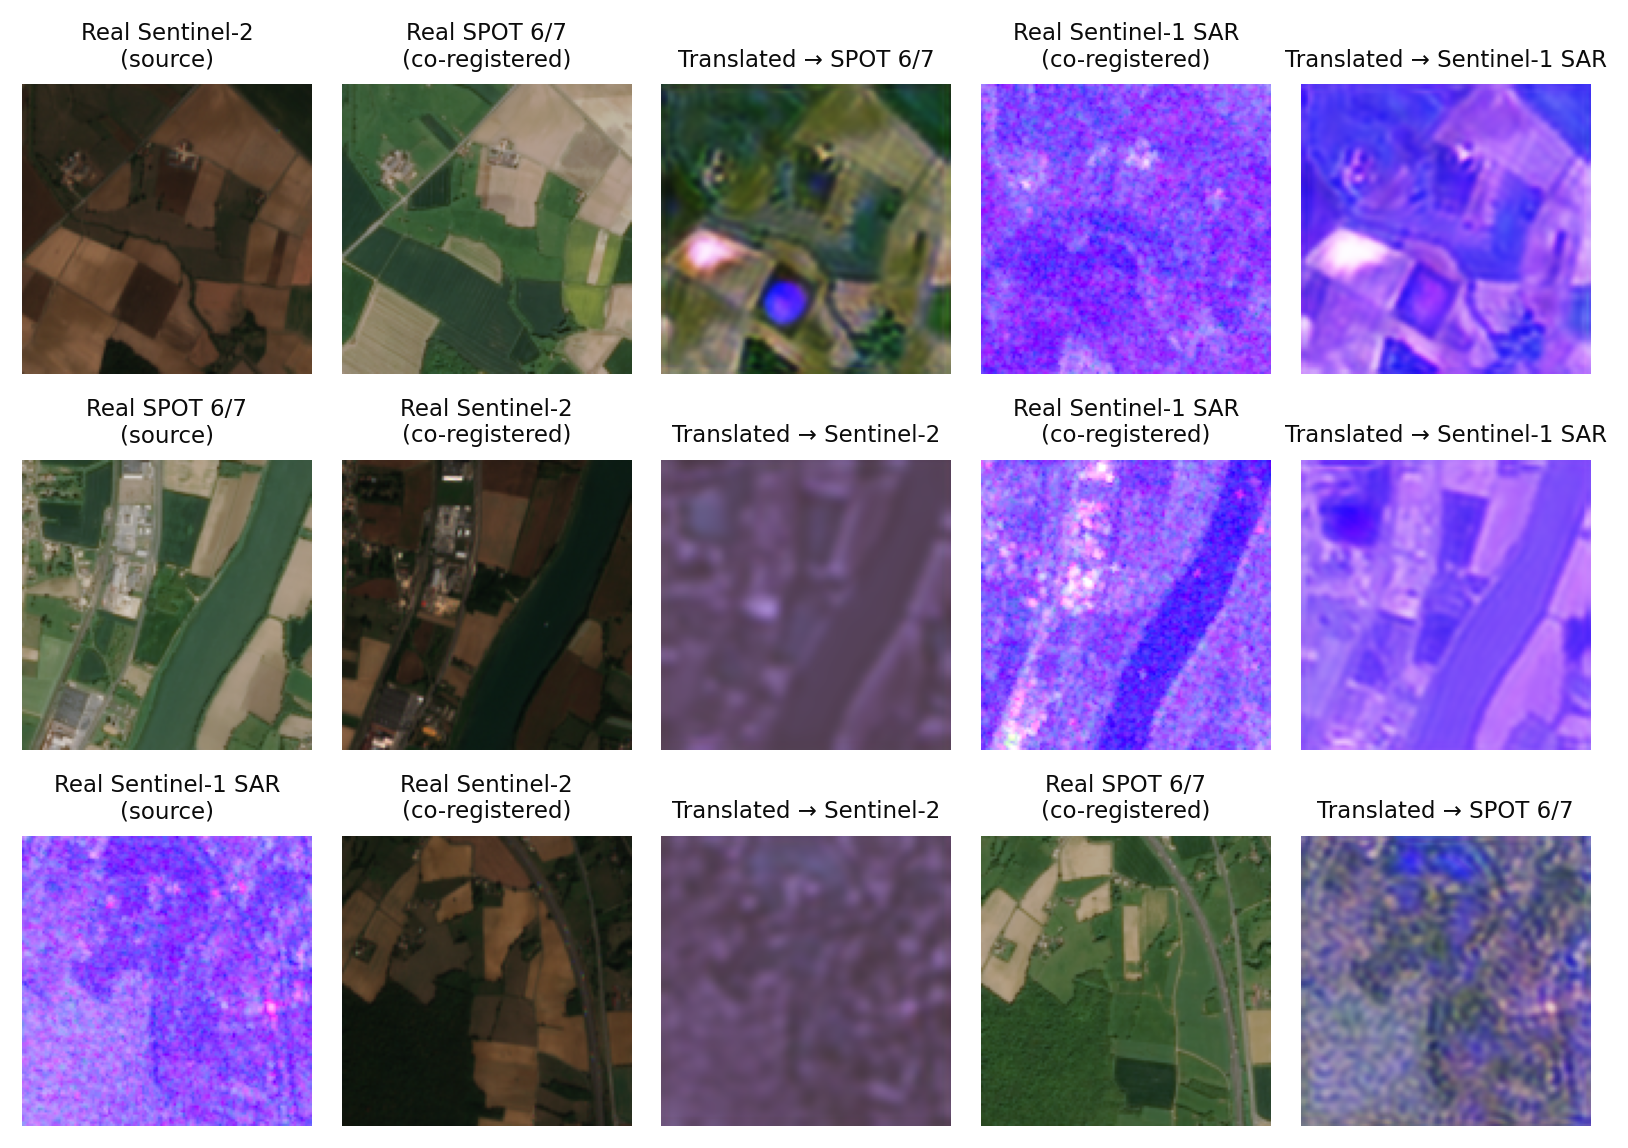
\includegraphics[width=\textwidth]{figures/fig_paired_translation.png}
\caption{Translations of one held-out patch per source domain (first column of each row) into the two other domains, shown next to the real co-registered patch of each target domain. The style is the centroid embedding of the target domain, and the patches were selected with a fixed random seed before inspection. Sentinel-1 patches are displayed with VV, VH, and the saturated difference channel as the red, green, and blue channels, respectively.}
\label{fig:paired}
\end{figure}

\begin{table}[t]
\centering
\caption{Translation into each target domain on held-out patches. PSNR (dB) against the co-registered real target patch is given for the translation, for the copied source (Copy), and for a constant target-mean image (Const.). Style is the share of outputs that the encoder assigns to the target domain, and Edge is the edge-map correlation with the source.}
\label{tab:gen}
\footnotesize
\setlength{\tabcolsep}{3.5pt}
\begin{tabular}{@{}lccccc@{}}
\toprule
\textbf{Pair} & \textbf{Transl.} & \textbf{Copy} & \textbf{Const.} & \textbf{Style} & \textbf{Edge} \\
\midrule
S2 $\rightarrow$ SPOT   & 14.6 & 13.1 & 17.2 & 57\% & 0.82 \\
S2 $\rightarrow$ SAR    & 14.6 & 5.7 & 20.5 & 18\% & 0.87 \\
SPOT $\rightarrow$ S2   & 13.5 & 13.1 & 17.8 & 29\% & 0.71 \\
SPOT $\rightarrow$ SAR  & 16.8 & 7.4 & 20.5 & 80\% & 0.82 \\
SAR $\rightarrow$ S2    & 13.3 & 5.7 & 17.8 & 12\% & 0.94 \\
SAR $\rightarrow$ SPOT  & 13.0 & 7.4 & 17.2 & 45\% & 0.92 \\
\bottomrule
\end{tabular}
\end{table}

Fig.~\ref{fig:paired} and Table~\ref{tab:gen} summarize the results for the generator. \emph{Structure is preserved:} the edge-map correlation between the source and the output ranges from 0.71 to 0.94, which is higher than the 0.61 to 0.70 observed between real patches of different sensors, and parcels, the river, and the road remain recognizable in the figure. \emph{The style vector is used:} with the correct target style, the PSNR is higher than with the style of the third domain for five of the six pairs (by 3.3 to 7.6~dB), and the translation is better than copying the source for all six pairs, most strongly for the pairs that involve SAR. \emph{Target radiometry is not reproduced:} for all six pairs, a constant image equal to the target-domain mean agrees better with the real target patch than the translation does (by 2.6 to 5.9~dB). In addition, the encoder assigns the outputs to the target domain in only 12\% to 80\% of the cases. Translations into Sentinel-2 appear as a blurred purple-gray haze whose channel means are identical for all three sources (within 0.001) and much brighter than those of real Sentinel-2 patches (by 0.59 in the blue channel on a $[-1,1]$ scale). The identity mapping of Sentinel-2 is also poorly reproduced (13.7~dB, compared with 20.3~dB for SPOT and 24.3~dB for SAR), which makes Sentinel-2 the weak point of the generator both as a source and as a target. Differences in acquisition date between the modalities limit the achievable pixel agreement, but they do not explain why the translation is worse than a constant image.

\emph{Continuity of the style space} was examined by interpolating between two domain centroids, $z(\alpha)=(1-\alpha)\bar z_a+\alpha\bar z_b$, renormalized to unit length, for 300 source patches. For the two pairs that involve SAR, the output changes smoothly and almost linearly (linearity ratio 0.91 and 0.96; monotone for 96\% and 100\% of the patches). For Sentinel-2 and SPOT, the change is about half as large, is concentrated in the first step from $\alpha=0$ to $\alpha=0.25$, and is monotone for only 41\% of the patches. The generator has 1.59~M parameters and the encoder 0.89~M, and one translation takes about 84~ms per patch on the CPU. Fig.~\ref{fig:interp} illustrates this interpolation for one held-out SPOT~6/7 source patch.

\begin{figure}[t]
\centering
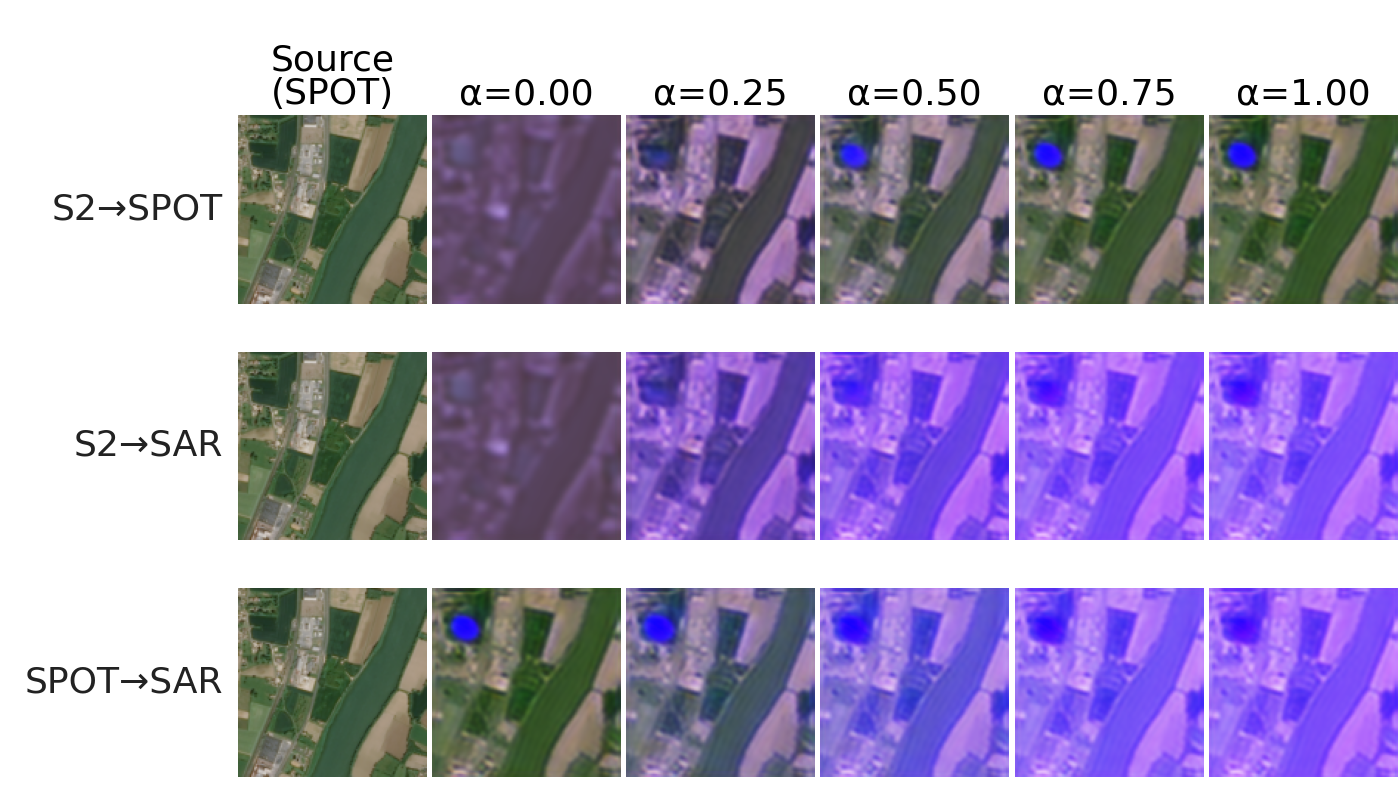
\includegraphics[width=0.85\textwidth]{figures/fig_interp_compact.png}
\caption{Interpolation of the style vector between two domain centroids, $z(\alpha)=(1-\alpha)\bar z_a+\alpha\bar z_b$, renormalized to unit length, applied to one held-out SPOT~6/7 source patch (first column). Each row corresponds to a domain pair $a \rightarrow b$, and $\alpha$ runs from the style of $a$ ($\alpha=0$) to the style of $b$ ($\alpha=1$). The patch was selected with a fixed random seed before inspection.}
\label{fig:interp}
\end{figure}

\section{Comparative Analysis}
Table~\ref{tab:gap} in Sec.~\ref{sec:gap} has already placed the proposed encoder-generator pair alongside the closest prior methods with respect to the properties that motivate this work. In the implementation, the design goals listed in Table~\ref{tab:gap} are met at the architectural level: training uses no domain labels, one generator serves all ordered pairs of three domains, and the domain code is a continuous 64-dimensional embedding. The quality of the results, however, cannot be compared with the cited methods, because none of them was trained on the same data and their published figures come from other datasets and tasks. Accordingly, no claim is made that the approach outperforms SS(DA)$^2$, StarGAN~v2, or the other methods.

\section{Limitations}
\label{sec:limitations}
Several limitations should be kept in mind when interpreting the results in Sec.~\ref{sec:results}. First, the held-out patches come from a single Sentinel-2 tile, whereas the training set is dominated by two other tiles; the results therefore combine model quality with a region shift, and in particular the domain centroids come from mostly different regions than the patches to which they are applied. Second, the modalities are not simultaneous, which limits pixel-level agreement with the co-registered reference, and the preprocessing introduces artifacts (a saturated SAR channel and a synthetic fourth SPOT channel). Third, each model was trained only once, with a short schedule (10 encoder and 12 generator epochs), a narrow network (base width 32), and a CPU-only laptop (Sec.~\ref{sec:setup}). The training loops are not seeded, the run-to-run variation is unknown, no ablation of the six generator losses was run, and no other translation method was trained on the same data for comparison. Fourth, PSNR and SSIM measure agreement with a co-registered image and not realism, and the style-transfer success rate is judged by the same encoder that conditions the generator, so it is only as reliable as that encoder. Fifth, only three sensor domains, one geographic setting, and $1{,}500$ of the $2{,}433$ locations are used; the larger MSC-France corpus foreseen for encoder pretraining was not used, and the angle-domain conditioning implemented in the framework was not exercised. Finally, generalization to unseen sensor pairs and downstream accuracy (Objectives~3--4) were not evaluated.

\section{Conclusion and Future Work}
This paper presented the first two components of a self-supervised, multi-domain adaptation framework for satellite imagery. The first is a contrastive domain encoder that learns continuous, label-free embeddings of sensor style from unlabeled multi-sensor patches. The second is a unified AdaIN-conditioned generator that uses this embedding, in place of the discrete domain labels required by prior multi-domain translators, to translate the content of a source patch into an arbitrary target style. Implemented and trained on real PASTIS-HD imagery across Sentinel-2, SPOT~6/7, and Sentinel-1 SAR, the framework meets its design goals at the architectural level: no domain labels, one model for all ordered domain pairs, and a continuous domain code. The measured quality is limited, however. The encoder identifies the sensor only moderately (65.8\% against 33.3\% by chance), and the generator preserves scene structure and uses the style vector but does not reproduce the radiometry of the target sensor, while translations into Sentinel-2 fail.

Building directly on these findings, future work will (i) replace the augmented-view positives of the encoder with sensor-aware positive pairs based on spatial and temporal proximity, and pretrain on the larger MSC-France corpus; (ii) correct the data issues identified here by using all PASTIS-HD patches with a tile-stratified split, temporally matched acquisitions, and a non-saturating SAR channel; (iii) train wider networks for longer on a GPU, with seeded and logged runs, loss ablations, and baselines trained on the same data; and (iv) carry out the leave-one-domain-pair-out and zero-shot (SpaceNet~6) generalization evaluation, together with the downstream crop-classification and segmentation evaluation, which constitute Objectives~3 and~4 of the broader project.

\bibliographystyle{splncs04}
\bibliography{references}

\end{document}
"
\ifdefined\ANON
\author{Anonymous Authors}
\authorrunning{Anonymous Authors}
\institute{Anonymous Institution}
\else
\author{Shivangi\textsuperscript{1} \and Benedict Tephila M.\textsuperscript{2} \and Naveen J.\textsuperscript{3}}
\authorrunning{S. et al.}
\institute{Department of Computer Science and Engineering,\\
CHRIST (Deemed to be University), Bangalore -- 560029, India\\
\textsuperscript{1}\email{shivangi.a@mtech.christuniversity.in},
\textsuperscript{2}\email{benedict.tephila@christuniversity.in},
\textsuperscript{3}\email{naveen.j@christuniversity.in}}
\fi

\maketitle

\begin{abstract}
Deep learning models for satellite image analysis are usually trained on imagery from a particular sensor, season, or geographic region, and their performance is known to deteriorate when the same land-cover classes are observed under a different acquisition domain. Current domain-adaptation approaches for satellite imagery generally depend on labeled target-domain data, on a discrete predefined set of domains, or on both. Such assumptions are hard to meet in practice, particularly for growing multi-sensor archives in which domain boundaries are not always clearly defined. This paper reports the first two components of a broader self-supervised multi-domain adaptation framework for satellite imagery. The first is (i) a continuous domain encoder that learns a label-free, continuous-valued style embedding directly from unlabeled multi-sensor image patches by means of a contrastive (InfoNCE) pretext task. The second is (ii) a unified conditional generator that translates the content of a source-domain patch into the style of an arbitrary target domain with a single Adaptive Instance Normalization (AdaIN)-modulated network, which is conditioned on the continuous embedding instead of a discrete domain label. Both networks were trained on a CPU using 1{,}200 patches per sensor from the real PASTIS-HD benchmark (Sentinel-2, SPOT~6/7, and Sentinel-1 SAR) and were evaluated on 300 held-out patches per sensor drawn from a largely different region. The encoder solves its pretext task, but it identifies the sensor only moderately well (65.8\% against 33.3\% by chance). The generator preserves scene structure and responds smoothly to interpolated styles for the pairs that involve SAR; however, it does not reproduce the radiometry of the target sensor. A constant image agrees better with the real target patch than the translation does, and translations into Sentinel-2 collapse to a source-independent color cast. Generalization to unseen sensor pairs and downstream accuracy lie outside the scope of this paper.
\keywords{domain adaptation \and self-supervised learning \and generative adversarial networks \and contrastive learning \and multi-sensor satellite imagery \and image-to-image translation}
\end{abstract}


\section{Introduction}

Satellite remote sensing has shifted from single-mission analysis to a setting in which optical and radar constellations -- Sentinel-2, Landsat, SPOT, and a growing set of commercial very-high-resolution (VHR) and synthetic aperture radar (SAR) platforms -- image the Earth's surface jointly and continuously. Deep learning models for land-cover classification, crop mapping, and change detection are therefore increasingly expected to operate across this heterogeneous, multi-sensor archive rather than only on the sensor on which they were trained.

Meeting this cross-sensor requirement is difficult in practice. Every sensor has its own radiometric calibration, spectral response, spatial resolution, and noise characteristics, and the resulting effects range from atmospheric haze and calibration drift in optical imagery to speckle noise and incidence-angle-dependent backscatter in SAR. Consequently, a model trained on the statistics of one sensor can lose a great deal of accuracy when it is applied to another sensor, even if the underlying land-cover classes are identical. Because acquiring and annotating imagery from every sensor of interest is costly, models often have to be adapted to a new domain with little or no labeled target-domain data.

Existing approaches to this problem fall broadly into two families. Domain-adaptation methods designed specifically for satellite imagery, such as multi-source standardization~\cite{tasar2020standardgan}, condition the translation on a discrete, manually assigned domain identity and have been shown to struggle with domain-pair combinations that were not seen during training. Self-supervised alternatives such as SS(DA)$^2$~\cite{zhang2023ssdada} need neither labels nor an explicit domain boundary, but they are formulated for translation between exactly two satellites at a time, so every new sensor pair requires separate training. In the wider image-to-image translation literature, StarGAN~\cite{choi2018stargan} and StarGAN~v2~\cite{choi2020starganv2} unify translation across many domains in a single generator, and StarGAN~v2 replaces discrete domain labels with a learned continuous style code. Both, however, are trained with supervised, discretely indexed domain labels, and they are evaluated on natural-image benchmarks (faces, animal faces) with visual-realism metrics, rather than on satellite imagery or on downstream task correctness. More recent diffusion-based translators~\cite{vinholi2024multisensor,kieu2025universal} improve translation quality, and the diffusion router~\cite{kieu2025universal} additionally routes between multiple domains. Nevertheless, these methods still operate over a discrete, pre-enumerated set of domains and incur the considerably higher inference cost of iterative diffusion sampling.

In summary, the literature does not yet provide a method that combines, for satellite imagery, three properties at once: label-free training, a continuous representation of the domain (rather than a fixed-cardinality, discretely labeled one), and a single generator capable of translating into an arbitrary target style. This gap motivates the present work.

We address the first two of these properties by carrying the self-supervised, label-free philosophy of SS(DA)$^2$ over from a pairwise setting to a continuous, StarGAN~v2-style unified generator that does not require discrete domain conditioning. Specifically, a contrastive domain encoder is pretrained on unlabeled multi-sensor patches to produce a continuous embedding of each patch's sensor/style characteristics. A single conditional generator, modulated through AdaIN by this embedding, then translates a source patch into the style of any target patch's embedding, including domain combinations that were not explicitly indexed during training. This paper reports the design, implementation, and held-out evaluation of these two components. The remaining objectives of the broader project, namely generalization testing on unseen sensor-pair combinations and downstream task evaluation, are implemented in the accompanying codebase but fall outside the scope of this paper.

The contributions of this paper are:
\begin{itemize}
\item A self-supervised contrastive domain encoder that yields continuous, label-free embeddings of sensor/style characteristics directly from unlabeled multi-sensor satellite patches.
\item A single, unified AdaIN-modulated conditional generator that is conditioned on this continuous embedding instead of a discrete domain code, which makes translation into an arbitrary target style possible without retraining for each domain pair.
\item A composite training objective that combines adversarial, style-reconstruction, cycle-consistency, semantic-preservation, identity, and edge-preservation losses and is designed to keep geospatial content intact while the sensor-specific style is changed.
\item An implementation and held-out evaluation on the real PASTIS-HD multi-sensor benchmark (Sentinel-2, SPOT~6/7, Sentinel-1~SAR) that reports both what the approach achieves (label-free continuous embeddings, structure-preserving and style-conditioned translation) and where it falls short (moderate sensor information in the embedding, target radiometry not reproduced).
\end{itemize}

\section{Related Work}

\subsection{Domain Adaptation for Satellite Imagery}
StandardGAN~\cite{tasar2020standardgan} tackles multi-source domain adaptation for semantic segmentation of VHR satellite images. It standardizes the data distribution of each source domain toward a common reference before downstream training. The method operates over a discrete, enumerated set of source domains and, according to its authors, has difficulty preserving image content faithfully and generalizing to sensor combinations that were not standardized against directly. SS(DA)$^2$~\cite{zhang2023ssdada}, the base paper on which the present framework builds, eliminates the need for labeled target data and an explicit domain boundary: it trains a contrastive, domain-agnostic GAN that translates between two satellite domains using only unlabeled imagery. Its central limitation, and the specific gap addressed in this paper, is that the formulation is pairwise. Each trained model supports exactly two satellites, so adding a new sensor to the archive requires an additional model.

\subsection{Multi-Domain Image-to-Image Translation}
StarGAN~\cite{choi2018stargan} was the first method to unify multi-domain translation in a single generator; it conditions the network on a discrete one-hot domain vector provided at both training and inference time. StarGAN~v2~\cite{choi2020starganv2} replaces this discrete label with a continuous style code, which is produced by a mapping network or a style encoder and injected into the generator through AdaIN~\cite{huang2017adain}; its authors report substantially more diverse and realistic synthesis. Both methods, however, are trained with supervised domain labels and are evaluated on natural-image datasets (human/animal faces) with visual-realism metrics (e.g., FID), rather than on satellite imagery or with a task-grounded correctness metric. Diffusion-based translators have since been proposed for multi-sensor optical imagery~\cite{vinholi2024multisensor} and for universal multi-domain routing~\cite{kieu2025universal}. Although they improve sample fidelity, the router in~\cite{kieu2025universal} still selects among a discrete, pre-specified set of domain experts, and diffusion sampling is computationally more expensive at inference than a single feed-forward GAN pass, which is relevant when large satellite mosaics are translated.

\section{Research Gap and Motivation}
\label{sec:gap}
Table~\ref{tab:gap} compares the properties of the most closely related methods with those targeted by this work. None of the prior methods reviewed here combines label-free training with a continuous (open-ended) domain representation in a single generator that is designed for, and evaluated on, satellite imagery. SS(DA)$^2$ provides the first property but not the second, since it is pairwise only. StarGAN~v2 provides the second but not the first, because it needs supervised discrete labels at training time, and it is neither designed for nor evaluated on remote-sensing data. StandardGAN targets satellite imagery but requires a discrete domain identity. Objectives~1 and~2 of the present project, a label-free continuous domain encoder and a single unified generator conditioned on that continuous embedding, are intended to close this particular combination of gaps. Objectives~3 and~4 (generalization to unseen domain-pair combinations and downstream task evaluation) build on this foundation but are outside the scope of this paper.

\begin{table}[t]
\centering
\caption{Qualitative comparison of the properties relevant to the identified research gap.}
\label{tab:gap}
\resizebox{\linewidth}{!}{%
\begin{tabular}{@{}lccc@{}}
\toprule
\textbf{Method} & \textbf{Label-free} & \textbf{Continuous domain repr.} & \textbf{Satellite-specific} \\
\midrule
StandardGAN~\cite{tasar2020standardgan}    & \ding{55} & \ding{55} & \ding{51} \\
SS(DA)$^2$~\cite{zhang2023ssdada}          & \ding{51} & \ding{55} (pairwise) & \ding{51} \\
StarGAN~\cite{choi2018stargan}             & \ding{55} & \ding{55} & \ding{55} \\
StarGAN~v2~\cite{choi2020starganv2}        & \ding{55} & \ding{51} & \ding{55} \\
\textbf{Proposed (Objectives 1--2)}        & \ding{51} & \ding{51} & \ding{51} \\
\bottomrule
\end{tabular}}
\end{table}

\section{Proposed Methodology}

\begin{figure}[t]
\centering
\resizebox{\textwidth}{!}{%
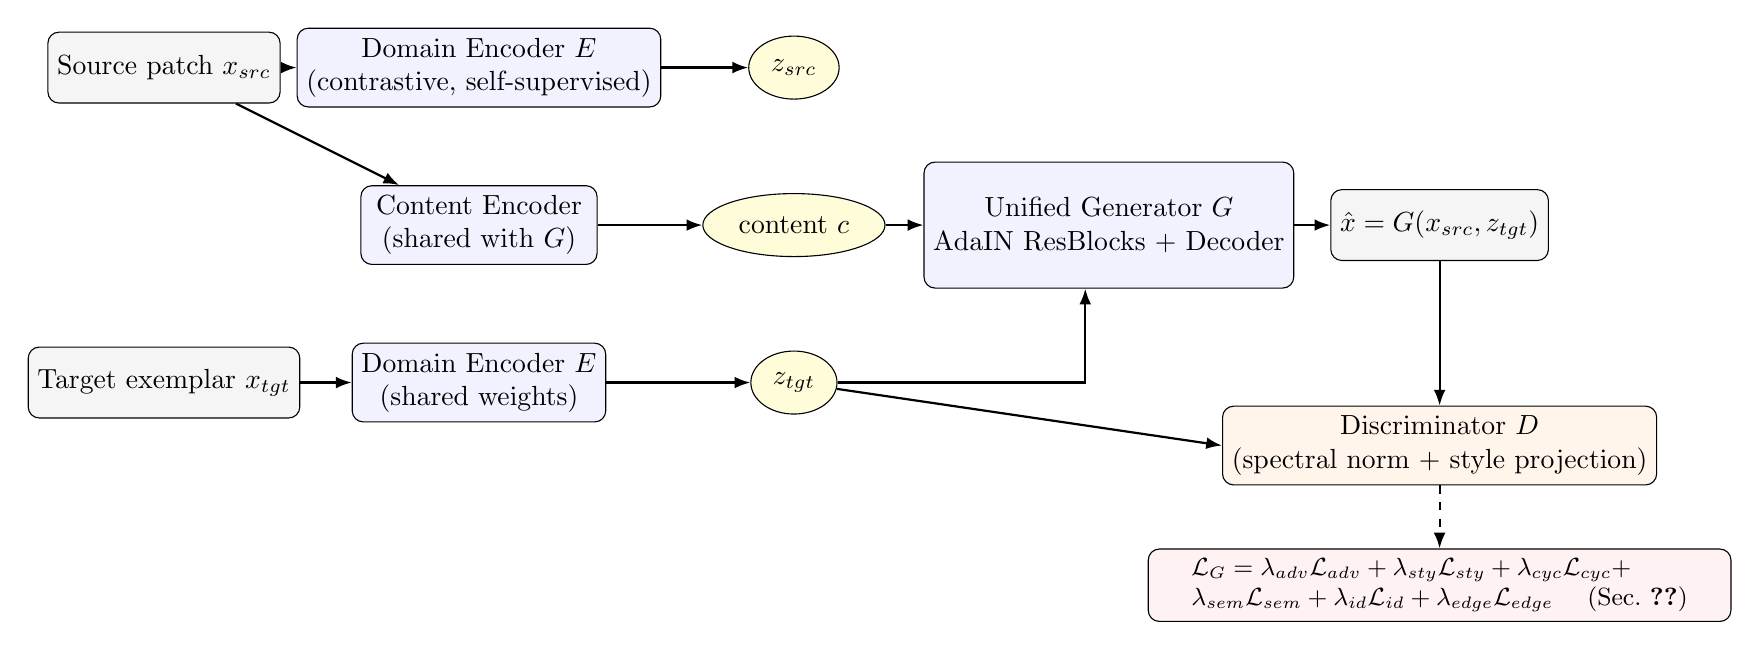
\begin{tikzpicture}[
  node distance=8mm and 10mm,
  box/.style={draw, rounded corners, align=center, minimum height=1.0cm, font=\normalsize, fill=blue!5},
  data/.style={draw, rounded corners, align=center, minimum height=0.9cm, font=\normalsize, fill=gray!8},
  vec/.style={draw, ellipse, align=center, minimum height=0.8cm, font=\normalsize, fill=yellow!15},
  lossbox/.style={draw, rounded corners, align=left, font=\small, fill=red!5},
  arr/.style={-{Latex[length=2mm]}, thick}
]
  \node[data]                              (xsrc) at (0,6)    {Source patch $x_{src}$};
  \node[data]                              (xtgt) at (0,2)    {Target exemplar $x_{tgt}$};

  \node[box, minimum width=3.0cm]          (E1)   at (4.0,6)  {Domain Encoder $E$\\(contrastive, self-supervised)};
  \node[box, minimum width=3.0cm]          (CE)   at (4.0,4)  {Content Encoder\\(shared with $G$)};
  \node[box, minimum width=3.0cm]          (E2)   at (4.0,2)  {Domain Encoder $E$\\(shared weights)};

  \node[vec]                               (zsrc) at (8.0,6)  {$z_{src}$};
  \node[vec]                               (c)    at (8.0,4)  {content $c$};
  \node[vec]                               (ztgt) at (8.0,2)  {$z_{tgt}$};

  \node[box, minimum width=3.2cm, minimum height=1.6cm] (G) at (12.0,4) {Unified Generator $G$\\AdaIN ResBlocks + Decoder};

  \node[data, minimum width=2.6cm]         (xfake) at (16.2,4) {$\hat{x} = G(x_{src}, z_{tgt})$};

  \node[box, fill=orange!8, minimum width=3.0cm] (D) at (16.2,1.2) {Discriminator $D$\\(spectral norm + style projection)};

  \draw[arr] (xsrc) -- (E1);
  \draw[arr] (xsrc) -- (CE);
  \draw[arr] (xtgt) -- (E2);
  \draw[arr] (E1) -- (zsrc);
  \draw[arr] (CE) -- (c);
  \draw[arr] (E2) -- (ztgt);
  \draw[arr] (c) -- (G);
  \draw[arr] (ztgt.east) -| ([xshift=-3mm]G.south);
  \draw[arr] (G) -- (xfake);
  \draw[arr] (xfake) -- (D);
  \draw[arr] (ztgt) -- (D.west);

  \node[lossbox, below=8mm of D, minimum width=7.4cm] (losses) {
    $\mathcal{L}_G = \lambda_{adv}\mathcal{L}_{adv} + \lambda_{sty}\mathcal{L}_{sty} + \lambda_{cyc}\mathcal{L}_{cyc} +$\\
    $\lambda_{sem}\mathcal{L}_{sem} + \lambda_{id}\mathcal{L}_{id} + \lambda_{edge}\mathcal{L}_{edge}$ \quad (Sec.~\ref{sec:objective})
  };
  \draw[arr, dashed] (D.south) -- (losses.north);
\end{tikzpicture}}
\caption{Simplified architecture of the two components reported in this paper: the self-supervised continuous domain encoder $E$ (Objective~1, Sec.~\ref{sec:encoder}) and the unified AdaIN-conditioned generator $G$ with its projection discriminator $D$ (Objective~2, Sec.~\ref{sec:generator}). For clarity, the figure omits two additional forward passes of the source embedding $z_{src}$ through $G$, which are used to compute the cycle-consistency and identity losses of Sec.~\ref{sec:objective}. Components that belong to later objectives of the project (leave-one-pair-out generalization testing and downstream task evaluation) are not shown, because they are outside the scope of this paper.}
\label{fig:architecture}
\end{figure}

Fig.~\ref{fig:architecture} shows the two components covered in this paper. A domain encoder $E$ maps an unlabeled image patch to a continuous style embedding. A content encoder, which is the downsampling path of the generator, extracts a domain-invariant spatial content code. A unified generator $G$ then combines the content of a source patch with the embedding of a target patch to synthesize a translation, which is assessed by a projection discriminator $D$.

\subsection{Self-Supervised Continuous Domain Encoder}
\label{sec:encoder}
The encoder $E_\theta$ receives an $H \times W$ patch with $C$ channels (4 in this implementation: three optical/SAR-derived channels plus one auxiliary channel, see Sec.~\ref{sec:dataset}) and outputs a continuous embedding $z \in \mathbb{R}^{64}$. An input-adapter convolution is followed by three stride-2 convolutional blocks (each Conv--InstanceNorm--LeakyReLU), which progressively reduce the spatial resolution while increasing the channel width. A squeeze-and-excitation (SE) block~\cite{hu2018senet} then recalibrates the channel-wise responses so that the encoder can attend to the most discriminative bands (e.g., near-infrared for vegetation, VV/VH ratio for SAR).

Instead of pooling to a class score, the encoder computes first- and second-order spatial statistics of the final feature map, namely the channel-wise mean $\mu$ and standard deviation $\sigma$. Together, they summarize the radiometric and textural style of the patch independently of its spatial content:
\begin{equation}
\mu_c = \frac{1}{HW}\sum_{i,j} h_{c,i,j}, \qquad
\sigma_c = \sqrt{\frac{1}{HW}\sum_{i,j}(h_{c,i,j}-\mu_c)^2 + \epsilon}
\label{eq:stats}
\end{equation}
where $h$ is the feature map after the SE block. The concatenated statistics $[\mu;\sigma]$ (optionally fused with a projected acquisition-angle feature when angle metadata are available; this option is unused in the sensor-only experiment reported here) pass through a multilayer perceptron projection head and are L2-normalized onto the unit hypersphere:
\begin{equation}
z = \frac{f_\phi([\mu;\sigma])}{\lVert f_\phi([\mu;\sigma]) \rVert_2}, \qquad z \in \mathbb{R}^{64}.
\label{eq:embed}
\end{equation}

The encoder is pretrained without domain labels, using a contrastive pretext task in the style of InfoNCE~\cite{oord2018cpc}. Two independently augmented views ($z_1, z_2$) of the same patch (random flips and 90\textdegree{} rotations) form a positive pair, whereas all other patches in the training batch serve as negatives:
\begin{equation}
\mathcal{L}_{con} = -\frac{1}{2B}\sum_{i=1}^{B}\Big[
\log\frac{e^{\,z_{1,i}\cdot z_{2,i}/\tau}}{\sum_{j} e^{\,z_{1,i}\cdot z_{2,j}/\tau}}
+
\log\frac{e^{\,z_{2,i}\cdot z_{1,i}/\tau}}{\sum_{j} e^{\,z_{2,i}\cdot z_{1,j}/\tau}}
\Big]
\label{eq:infonce}
\end{equation}
where $B$ is the batch size and $\tau$ is a temperature hyperparameter. Since the positive/negative structure comes purely from data augmentation and not from sensor labels, the embedding space is learned without any supervision of domain identity. At inference time, any patch, whether from a domain seen during training or not, can be projected into the same continuous space.

\subsection{Unified Conditional Generator}
\label{sec:generator}
The generator $G_\psi$ receives a source patch $x_{src}$ and a target embedding $z_{tgt}$, which the frozen encoder $E$ produces from a target-domain exemplar, and it synthesizes a translated patch $\hat{x} = G_\psi(x_{src}, z_{tgt})$. One generator instance is shared across all domains, and the target style is determined entirely by $z_{tgt}$. Translation into any domain that the encoder can embed, and not only the domains enumerated at training time, therefore requires neither architectural changes nor additional parameters.

The content path follows an encoder-bottleneck-decoder design in the spirit of StarGAN~v2~\cite{choi2020starganv2}, adapted to be label-free. A content encoder with reflection-padded convolutions and instance normalization downsamples $x_{src}$ into a domain-invariant content code $c = \mathrm{Enc}_c(x_{src})$. This code passes through four residual blocks modulated by Adaptive Instance Normalization (AdaIN)~\cite{huang2017adain}, which injects the target style at every block:
\begin{equation}
\mathrm{AdaIN}(h, z) = \gamma(z)\cdot\frac{h - \mu(h)}{\sigma(h)} + \beta(z)
\label{eq:adain}
\end{equation}
where $\mu(h), \sigma(h)$ are the per-channel instance statistics of the intermediate feature map $h$, and $\gamma(z) = W_\gamma z + b_\gamma$, $\beta(z) = W_\beta z + b_\beta$ are affine parameters regressed from the continuous embedding. The decoder mirrors the encoder with two AdaIN-modulated upsampling stages. It uses bilinear upsampling, instead of nearest-neighbor or transposed-convolution upsampling, to avoid checkerboard artifacts, and it ends with a reflection-padded output convolution with a $\tanh$ activation.

\subsection{Discriminator with Continuous Style Projection}
The discriminator $D_\xi$ is a multi-scale PatchGAN in which spectral normalization~\cite{miyato2018spectral} is applied to every convolutional layer; this stabilizes adversarial training by bounding the Lipschitz constant of each layer. Besides an unconditional real/fake head, $D_\xi$ projects its intermediate features onto the conditioning embedding $z$:
\begin{equation}
D_\xi(x, z) = D_{uncond}(x) + \frac{\langle \phi(x), W_{proj}\,z\rangle}{\sqrt{d}}
\label{eq:disc}
\end{equation}
where $\phi(x)$ is the penultimate feature map of the discriminator, $W_{proj}$ is a learned linear projection of the embedding, and $d$ is the feature dimension. This term penalizes translations whose visual style does not match the conditioning embedding $z$, and it thereby complements the style-reconstruction signal obtained from the encoder (Sec.~\ref{sec:objective}).

\subsection{Composite Training Objective}
\label{sec:objective}
The generator is trained with a weighted sum of six loss terms. Each term targets a specific failure mode observed in unconstrained multi-domain translation.

\emph{Adversarial loss} (least-squares GAN~\cite{mao2017lsgan}), which encourages $\hat{x}$ to be indistinguishable from real target-domain patches under the style-conditioned discriminator:
\begin{align}
\mathcal{L}_D &= \tfrac{1}{2}\mathbb{E}\big[(D_\xi(x_{tgt}, z_{tgt}) - 1)^2\big] + \tfrac{1}{2}\mathbb{E}\big[D_\xi(\hat{x}, z_{tgt})^2\big] \\
\mathcal{L}_{adv} &= \mathbb{E}\big[(D_\xi(\hat{x}, z_{tgt}) - 1)^2\big]
\label{eq:adv}
\end{align}

\emph{Style-reconstruction loss}, which requires that the target style can be measured in the output by re-encoding it:
\begin{equation}
\mathcal{L}_{sty} = \mathbb{E}\,\lVert E(\hat{x}) - z_{tgt} \rVert_1
\label{eq:sty}
\end{equation}

\emph{Cycle-consistency loss}~\cite{zhu2017cyclegan}, which translates $\hat{x}$ back toward the source style and requires the original patch to be recovered, thereby discouraging mode collapse across domains:
\begin{equation}
\mathcal{L}_{cyc} = \mathbb{E}\,\lVert G(\hat{x}, z_{src}) - x_{src} \rVert_1
\label{eq:cyc}
\end{equation}

\emph{Semantic-preservation loss}, which penalizes drift of the domain-invariant content code between the source and the translation, so that the geospatial layout (parcel boundaries, roads) is not altered by the style change:
\begin{equation}
\mathcal{L}_{sem} = \mathbb{E}\,\lVert \mathrm{Enc}_c(\hat{x}) - \mathrm{Enc}_c(x_{src}) \rVert_1
\label{eq:sem}
\end{equation}

\emph{Identity loss}, which requires that conditioning the generator on the source's own style leaves the patch unchanged:
\begin{equation}
\mathcal{L}_{id} = \mathbb{E}\,\lVert G(x_{src}, z_{src}) - x_{src} \rVert_1
\label{eq:id}
\end{equation}

\emph{Edge-preservation loss}, which compares the Sobel gradient magnitudes of $\hat{x}$ and $x_{src}$ in order to keep agricultural parcel boundaries and road edges sharp:
\begin{equation}
\mathcal{L}_{edge} = \mathbb{E}\,\lVert \nabla_{Sobel}(\hat{x}) - \nabla_{Sobel}(x_{src}) \rVert_1
\label{eq:edge}
\end{equation}

The total generator objective is
\begin{align}
\mathcal{L}_G ={}& \lambda_{adv}\mathcal{L}_{adv} + \lambda_{sty}\mathcal{L}_{sty} + \lambda_{cyc}\mathcal{L}_{cyc} \notag \\
& + \lambda_{sem}\mathcal{L}_{sem} + \lambda_{id}\mathcal{L}_{id} + \lambda_{edge}\mathcal{L}_{edge}
\label{eq:total}
\end{align}
with the weights listed in Table~\ref{tab:hyperparams}. In addition, the framework defines a geometric (SSIM-style) preservation loss $\mathcal{L}_{geo}$, which is activated when the source or the target domain is an off-nadir viewing-angle domain. The PASTIS-HD experiment reported in Sec.~\ref{sec:results} uses only sensor domains, so $\mathcal{L}_{geo}$ is inactive ($\lambda_{geo}\mathcal{L}_{geo}=0$) for the results presented here.

\section{Dataset and Preprocessing}
\label{sec:dataset}
The experiments use patches derived from PASTIS-HD~\cite{garnot2021panoptic,astruc2024omnisat}, a real and publicly released benchmark of $2{,}433$ co-registered agricultural-parcel locations across metropolitan France. Each location is available as a Sentinel-2 optical time series, a Sentinel-1 SAR time series, and, in the HD extension, a very-high-resolution SPOT~6/7 image. A conversion pipeline in the accompanying codebase matches patches across modalities by their shared patch identifier and exports one $128\times128$, 4-channel tensor per modality and location. For Sentinel-2, only the Red, Green, Blue, and near-infrared bands of a single temporal acquisition are kept. The SPOT~6/7 imagery is resized from its native $1280\times1280$ resolution to $128\times128$ and supplemented with a synthetic near-infrared proxy channel. The VV and VH polarizations of Sentinel-1 SAR are extended with a derived ratio channel and an average channel, and are normalized from decibel units. All modalities are scaled to $[-1,1]$. Of the up to $2{,}433$ available locations, this experiment converts $1{,}500$ per domain, a number limited by the patch cap of the conversion pipeline (Table~\ref{tab:dataset}). The converted patches are the first $1{,}500$ in identifier order and originate from three Sentinel-2 tiles. An 80/20 split by identifier order yields $1{,}200$ training patches and $300$ held-out patches per domain. As a consequence, all held-out patches belong to a single tile (T31TFM) that is only marginally represented in the training data, so the held-out evaluation is largely a test on a different region. The modalities are co-registered but not simultaneous: the first Sentinel-1 acquisition follows the first Sentinel-2 acquisition by 11~days at the median, and the SPOT imagery dates from 2019, whereas the Sentinel data begin in September 2018. After conversion, the SAR difference channel is saturated at $+1$ for 97.9\% of its values. Training-split patches are augmented on the fly with random horizontal and vertical flips, random 90\textdegree{} rotations, and small per-channel Gaussian radiometric noise ($\sigma \sim \mathcal{U}[0, 0.01]$).

\begin{table}[t]
\centering
\caption{Converted PASTIS-HD patches used in this study.}
\label{tab:dataset}
\begin{tabular}{@{}lccc@{}}
\toprule
\textbf{Domain} & \textbf{Modality} & \textbf{Channels} & \textbf{Patches} \\
\midrule
Sentinel-2       & Multispectral optical (R,G,B,NIR) & 4 & 1{,}500 \\
SPOT 6/7         & VHR optical (+NIR proxy)          & 4 & 1{,}500 \\
Sentinel-1 SAR   & C-band radar (VV, VH, ratio, avg) & 4 & 1{,}500 \\
\bottomrule
\end{tabular}
\end{table}

\section{Experimental Setup}
\label{sec:setup}
The framework is implemented in Python~3.13 with PyTorch~$\geq$2.4; NumPy, SciPy, Pillow, Matplotlib, and PyYAML are used for data handling, preprocessing, and visualization. A single command-line entry point orchestrates training: it first runs domain-encoder pretraining and then trains the generator and discriminator jointly. All training and evaluation were run on the CPU of a laptop (Intel Core i7-9750H, 6 cores, 7.8~GB RAM, Windows~11) with a CPU-only PyTorch build. The channel width of the generator and discriminator was deliberately kept narrow (base width 32) so that training remains tractable at this compute scale, and not in order to match a specific reported baseline configuration. Table~\ref{tab:hyperparams} lists the hyperparameters used for the results in Sec.~\ref{sec:results}.

\begin{table}[t]
\centering
\caption{Training hyperparameters.}
\label{tab:hyperparams}
\begin{tabular}{@{}ll@{}}
\toprule
\textbf{Stage 1 -- Domain Encoder} & \textbf{Value} \\
\midrule
Embedding dimension $d$            & 64 \\
Optimizer                          & AdamW \\
Learning rate                      & $5\times10^{-4}$ \\
Weight decay                       & $1\times10^{-4}$ \\
Contrastive temperature $\tau$     & 0.07 \\
Epochs                             & 10 \\
\midrule
\textbf{Stage 2 -- Generator / Discriminator} & \textbf{Value} \\
\midrule
Base channel width                 & 32 \\
Residual blocks                    & 4 \\
Optimizer ($G$, $D$)               & Adam ($\beta_1{=}0.5$, $\beta_2{=}0.999$) \\
Learning rate ($G$, $D$)           & $3\times10^{-4}$ \\
LR schedule                        & Cosine annealing, $\eta_{min}{=}10^{-5}$ \\
Gradient clipping (max norm)       & 1.0 \\
Epochs                             & 12 \\
Batch size                         & 8 \\
$\lambda_{adv},\lambda_{sty},\lambda_{id}$ & 1.0 each \\
$\lambda_{sem}$, $\lambda_{edge}$  & 2.0 each \\
$\lambda_{cyc}$                    & 10.0 \\
\bottomrule
\end{tabular}
\end{table}

\section{Results and Discussion}
\label{sec:results}
All results were measured on the 300 held-out patches per domain with a fixed protocol, and each is a single measurement of one trained model. The style of a target domain is defined as the L2-normalized mean of the embeddings of its 1{,}200 training patches (the domain \emph{centroid}); domain labels and co-registered patches are used only for evaluation. Image metrics are computed on images rescaled to $[0,1]$ against the co-registered real target patch, and two reference baselines are included: the untranslated source patch (``Copy'') and a constant image equal to the mean of the target domain (``Const.'').

\subsection{Domain encoder (Objective~1)}
Table~\ref{tab:enc} summarizes the results for the encoder. It solves its contrastive task on held-out patches (loss 0.24, against 2.08 for an uninformative embedding; 88.2\% top-1 retrieval of the second view among 900 patches), and its embeddings are distributed continuously over the hypersphere and do not form three tight clusters. However, they describe the sensor only moderately well: the nearest centroid assigns 65.8\% of the held-out patches to the correct sensor, against 33.3\% by chance; the sensors overlap (silhouette coefficient 0.11); and the effective dimensionality is about four. Retrieval of the co-registered patch from another sensor is at chance level, which indicates that the embedding does not carry scene content shared across sensors. A likely explanation, which was not tested, is that instance discrimination rewards distinguishing individual patches and includes no term that groups the patches of one sensor; the proximity-based positive pairs foreseen in the project plan were not used.

\begin{table}[t]
\centering
\caption{Domain encoder evaluated on 300 held-out patches per domain (S2: Sentinel-2).}
\label{tab:enc}
\begin{tabular}{@{}lc@{}}
\toprule
\textbf{Measurement} & \textbf{Result} \\
\midrule
Held-out InfoNCE loss (batch 8; chance 2.08)        & 0.24 \\
Top-1 instance retrieval among 900 patches          & 88.2\% \\
Nearest-centroid domain accuracy (chance 33.3\%)    & 65.8\% \\
\quad recall S2 / SPOT / SAR                        & 62.7 / 74.3 / 60.3\% \\
5-nearest-neighbor domain accuracy                  & 63.7\% \\
Cosine similarity within / between domains          & 0.32 / 0.04 \\
Silhouette coefficient (cosine distance)            & 0.11 \\
Participation ratio (of 64 dimensions)              & 3.85 \\
Same-location retrieval across sensors, top-1       & 0.3\% (chance 0.3\%) \\
\bottomrule
\end{tabular}
\end{table}

\subsection{Conditional generator (Objective~2)}
\begin{figure}[t]
\centering
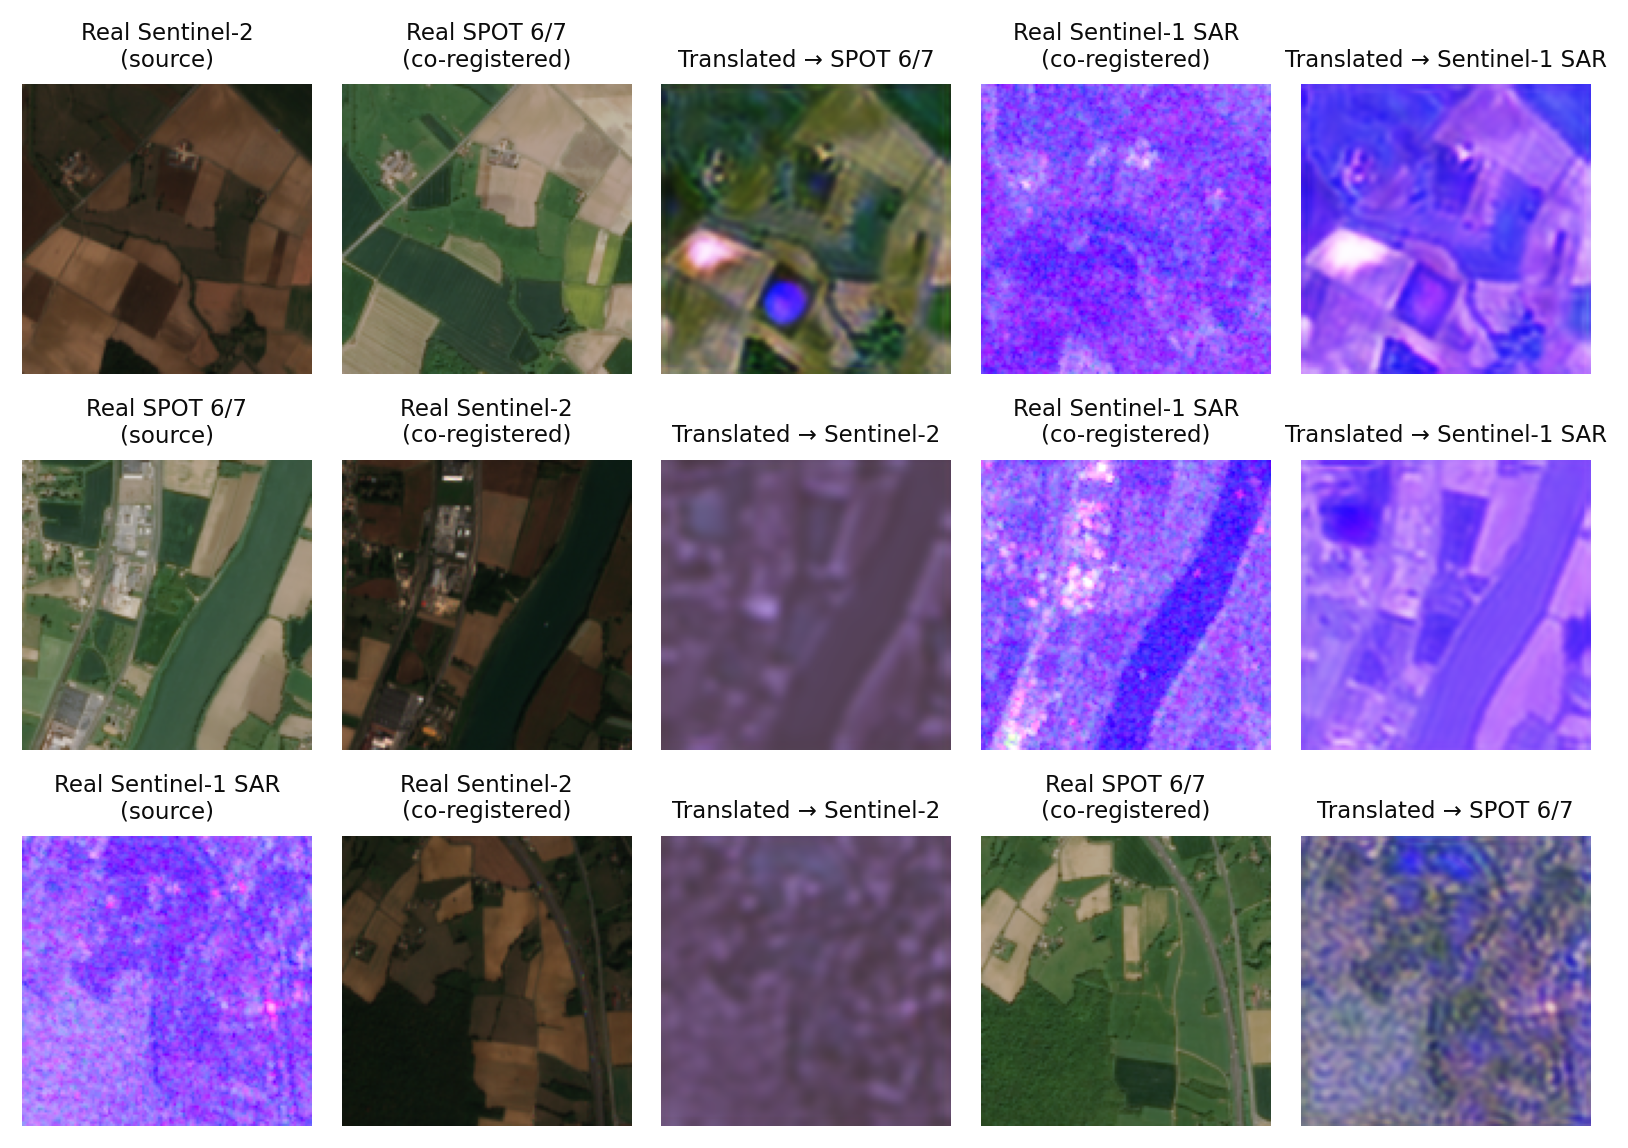
\includegraphics[width=\textwidth]{figures/fig_paired_translation.png}
\caption{Translations of one held-out patch per source domain (first column of each row) into the two other domains, shown next to the real co-registered patch of each target domain. The style is the centroid embedding of the target domain, and the patches were selected with a fixed random seed before inspection. Sentinel-1 patches are displayed with VV, VH, and the saturated difference channel as the red, green, and blue channels, respectively.}
\label{fig:paired}
\end{figure}

\begin{table}[t]
\centering
\caption{Translation into each target domain on held-out patches. PSNR (dB) against the co-registered real target patch is given for the translation, for the copied source (Copy), and for a constant target-mean image (Const.). Style is the share of outputs that the encoder assigns to the target domain, and Edge is the edge-map correlation with the source.}
\label{tab:gen}
\footnotesize
\setlength{\tabcolsep}{3.5pt}
\begin{tabular}{@{}lccccc@{}}
\toprule
\textbf{Pair} & \textbf{Transl.} & \textbf{Copy} & \textbf{Const.} & \textbf{Style} & \textbf{Edge} \\
\midrule
S2 $\rightarrow$ SPOT   & 14.6 & 13.1 & 17.2 & 57\% & 0.82 \\
S2 $\rightarrow$ SAR    & 14.6 & 5.7 & 20.5 & 18\% & 0.87 \\
SPOT $\rightarrow$ S2   & 13.5 & 13.1 & 17.8 & 29\% & 0.71 \\
SPOT $\rightarrow$ SAR  & 16.8 & 7.4 & 20.5 & 80\% & 0.82 \\
SAR $\rightarrow$ S2    & 13.3 & 5.7 & 17.8 & 12\% & 0.94 \\
SAR $\rightarrow$ SPOT  & 13.0 & 7.4 & 17.2 & 45\% & 0.92 \\
\bottomrule
\end{tabular}
\end{table}

Fig.~\ref{fig:paired} and Table~\ref{tab:gen} summarize the results for the generator. \emph{Structure is preserved:} the edge-map correlation between the source and the output ranges from 0.71 to 0.94, which is higher than the 0.61 to 0.70 observed between real patches of different sensors, and parcels, the river, and the road remain recognizable in the figure. \emph{The style vector is used:} with the correct target style, the PSNR is higher than with the style of the third domain for five of the six pairs (by 3.3 to 7.6~dB), and the translation is better than copying the source for all six pairs, most strongly for the pairs that involve SAR. \emph{Target radiometry is not reproduced:} for all six pairs, a constant image equal to the target-domain mean agrees better with the real target patch than the translation does (by 2.6 to 5.9~dB). In addition, the encoder assigns the outputs to the target domain in only 12\% to 80\% of the cases. Translations into Sentinel-2 appear as a blurred purple-gray haze whose channel means are identical for all three sources (within 0.001) and much brighter than those of real Sentinel-2 patches (by 0.59 in the blue channel on a $[-1,1]$ scale). The identity mapping of Sentinel-2 is also poorly reproduced (13.7~dB, compared with 20.3~dB for SPOT and 24.3~dB for SAR), which makes Sentinel-2 the weak point of the generator both as a source and as a target. Differences in acquisition date between the modalities limit the achievable pixel agreement, but they do not explain why the translation is worse than a constant image.

\emph{Continuity of the style space} was examined by interpolating between two domain centroids, $z(\alpha)=(1-\alpha)\bar z_a+\alpha\bar z_b$, renormalized to unit length, for 300 source patches. For the two pairs that involve SAR, the output changes smoothly and almost linearly (linearity ratio 0.91 and 0.96; monotone for 96\% and 100\% of the patches). For Sentinel-2 and SPOT, the change is about half as large, is concentrated in the first step from $\alpha=0$ to $\alpha=0.25$, and is monotone for only 41\% of the patches. The generator has 1.59~M parameters and the encoder 0.89~M, and one translation takes about 84~ms per patch on the CPU. Fig.~\ref{fig:interp} illustrates this interpolation for one held-out SPOT~6/7 source patch.

\begin{figure}[t]
\centering
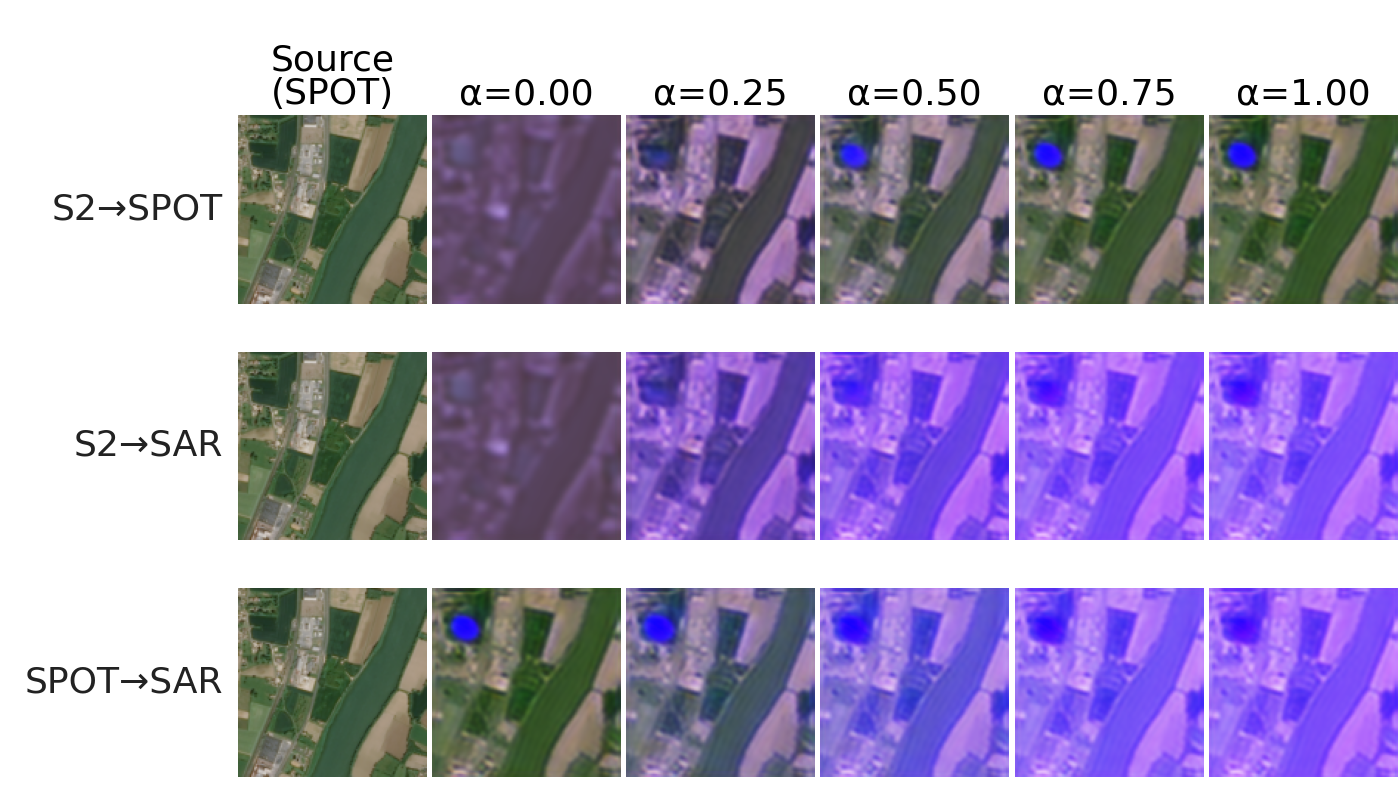
\includegraphics[width=0.85\textwidth]{figures/fig_interp_compact.png}
\caption{Interpolation of the style vector between two domain centroids, $z(\alpha)=(1-\alpha)\bar z_a+\alpha\bar z_b$, renormalized to unit length, applied to one held-out SPOT~6/7 source patch (first column). Each row corresponds to a domain pair $a \rightarrow b$, and $\alpha$ runs from the style of $a$ ($\alpha=0$) to the style of $b$ ($\alpha=1$). The patch was selected with a fixed random seed before inspection.}
\label{fig:interp}
\end{figure}

\section{Comparative Analysis}
Table~\ref{tab:gap} in Sec.~\ref{sec:gap} has already placed the proposed encoder-generator pair alongside the closest prior methods with respect to the properties that motivate this work. In the implementation, the design goals listed in Table~\ref{tab:gap} are met at the architectural level: training uses no domain labels, one generator serves all ordered pairs of three domains, and the domain code is a continuous 64-dimensional embedding. The quality of the results, however, cannot be compared with the cited methods, because none of them was trained on the same data and their published figures come from other datasets and tasks. Accordingly, no claim is made that the approach outperforms SS(DA)$^2$, StarGAN~v2, or the other methods.

\section{Limitations}
\label{sec:limitations}
Several limitations should be kept in mind when interpreting the results in Sec.~\ref{sec:results}. First, the held-out patches come from a single Sentinel-2 tile, whereas the training set is dominated by two other tiles; the results therefore combine model quality with a region shift, and in particular the domain centroids come from mostly different regions than the patches to which they are applied. Second, the modalities are not simultaneous, which limits pixel-level agreement with the co-registered reference, and the preprocessing introduces artifacts (a saturated SAR channel and a synthetic fourth SPOT channel). Third, each model was trained only once, with a short schedule (10 encoder and 12 generator epochs), a narrow network (base width 32), and a CPU-only laptop (Sec.~\ref{sec:setup}). The training loops are not seeded, the run-to-run variation is unknown, no ablation of the six generator losses was run, and no other translation method was trained on the same data for comparison. Fourth, PSNR and SSIM measure agreement with a co-registered image and not realism, and the style-transfer success rate is judged by the same encoder that conditions the generator, so it is only as reliable as that encoder. Fifth, only three sensor domains, one geographic setting, and $1{,}500$ of the $2{,}433$ locations are used; the larger MSC-France corpus foreseen for encoder pretraining was not used, and the angle-domain conditioning implemented in the framework was not exercised. Finally, generalization to unseen sensor pairs and downstream accuracy (Objectives~3--4) were not evaluated.

\section{Conclusion and Future Work}
This paper presented the first two components of a self-supervised, multi-domain adaptation framework for satellite imagery. The first is a contrastive domain encoder that learns continuous, label-free embeddings of sensor style from unlabeled multi-sensor patches. The second is a unified AdaIN-conditioned generator that uses this embedding, in place of the discrete domain labels required by prior multi-domain translators, to translate the content of a source patch into an arbitrary target style. Implemented and trained on real PASTIS-HD imagery across Sentinel-2, SPOT~6/7, and Sentinel-1 SAR, the framework meets its design goals at the architectural level: no domain labels, one model for all ordered domain pairs, and a continuous domain code. The measured quality is limited, however. The encoder identifies the sensor only moderately (65.8\% against 33.3\% by chance), and the generator preserves scene structure and uses the style vector but does not reproduce the radiometry of the target sensor, while translations into Sentinel-2 fail.

Building directly on these findings, future work will (i) replace the augmented-view positives of the encoder with sensor-aware positive pairs based on spatial and temporal proximity, and pretrain on the larger MSC-France corpus; (ii) correct the data issues identified here by using all PASTIS-HD patches with a tile-stratified split, temporally matched acquisitions, and a non-saturating SAR channel; (iii) train wider networks for longer on a GPU, with seeded and logged runs, loss ablations, and baselines trained on the same data; and (iv) carry out the leave-one-domain-pair-out and zero-shot (SpaceNet~6) generalization evaluation, together with the downstream crop-classification and segmentation evaluation, which constitute Objectives~3 and~4 of the broader project.

\bibliographystyle{splncs04}
\bibliography{references}

\end{document}
"
\ifdefined\ANON
\author{Anonymous Authors}
\authorrunning{Anonymous Authors}
\institute{Anonymous Institution}
\else
\author{Shivangi\textsuperscript{1} \and Benedict Tephila M.\textsuperscript{2} \and Naveen J.\textsuperscript{3}}
\authorrunning{S. et al.}
\institute{Department of Computer Science and Engineering,\\
CHRIST (Deemed to be University), Bangalore -- 560029, India\\
\textsuperscript{1}\email{shivangi.a@mtech.christuniversity.in},
\textsuperscript{2}\email{benedict.tephila@christuniversity.in},
\textsuperscript{3}\email{naveen.j@christuniversity.in}}
\fi

\maketitle

\begin{abstract}
Deep learning models for satellite image analysis are usually trained on imagery from a particular sensor, season, or geographic region, and their performance is known to deteriorate when the same land-cover classes are observed under a different acquisition domain. Current domain-adaptation approaches for satellite imagery generally depend on labeled target-domain data, on a discrete predefined set of domains, or on both. Such assumptions are hard to meet in practice, particularly for growing multi-sensor archives in which domain boundaries are not always clearly defined. This paper reports the first two components of a broader self-supervised multi-domain adaptation framework for satellite imagery. The first is (i) a continuous domain encoder that learns a label-free, continuous-valued style embedding directly from unlabeled multi-sensor image patches by means of a contrastive (InfoNCE) pretext task. The second is (ii) a unified conditional generator that translates the content of a source-domain patch into the style of an arbitrary target domain with a single Adaptive Instance Normalization (AdaIN)-modulated network, which is conditioned on the continuous embedding instead of a discrete domain label. Both networks were trained on a CPU using 1{,}200 patches per sensor from the real PASTIS-HD benchmark (Sentinel-2, SPOT~6/7, and Sentinel-1 SAR) and were evaluated on 300 held-out patches per sensor drawn from a largely different region. The encoder solves its pretext task, but it identifies the sensor only moderately well (65.8\% against 33.3\% by chance). The generator preserves scene structure and responds smoothly to interpolated styles for the pairs that involve SAR; however, it does not reproduce the radiometry of the target sensor. A constant image agrees better with the real target patch than the translation does, and translations into Sentinel-2 collapse to a source-independent color cast. Generalization to unseen sensor pairs and downstream accuracy lie outside the scope of this paper.
\keywords{domain adaptation \and self-supervised learning \and generative adversarial networks \and contrastive learning \and multi-sensor satellite imagery \and image-to-image translation}
\end{abstract}


\section{Introduction}

Satellite remote sensing has shifted from single-mission analysis to a setting in which optical and radar constellations -- Sentinel-2, Landsat, SPOT, and a growing set of commercial very-high-resolution (VHR) and synthetic aperture radar (SAR) platforms -- image the Earth's surface jointly and continuously. Deep learning models for land-cover classification, crop mapping, and change detection are therefore increasingly expected to operate across this heterogeneous, multi-sensor archive rather than only on the sensor on which they were trained.

Meeting this cross-sensor requirement is difficult in practice. Every sensor has its own radiometric calibration, spectral response, spatial resolution, and noise characteristics, and the resulting effects range from atmospheric haze and calibration drift in optical imagery to speckle noise and incidence-angle-dependent backscatter in SAR. Consequently, a model trained on the statistics of one sensor can lose a great deal of accuracy when it is applied to another sensor, even if the underlying land-cover classes are identical. Because acquiring and annotating imagery from every sensor of interest is costly, models often have to be adapted to a new domain with little or no labeled target-domain data.

Existing approaches to this problem fall broadly into two families. Domain-adaptation methods designed specifically for satellite imagery, such as multi-source standardization~\cite{tasar2020standardgan}, condition the translation on a discrete, manually assigned domain identity and have been shown to struggle with domain-pair combinations that were not seen during training. Self-supervised alternatives such as SS(DA)$^2$~\cite{zhang2023ssdada} need neither labels nor an explicit domain boundary, but they are formulated for translation between exactly two satellites at a time, so every new sensor pair requires separate training. In the wider image-to-image translation literature, StarGAN~\cite{choi2018stargan} and StarGAN~v2~\cite{choi2020starganv2} unify translation across many domains in a single generator, and StarGAN~v2 replaces discrete domain labels with a learned continuous style code. Both, however, are trained with supervised, discretely indexed domain labels, and they are evaluated on natural-image benchmarks (faces, animal faces) with visual-realism metrics, rather than on satellite imagery or on downstream task correctness. More recent diffusion-based translators~\cite{vinholi2024multisensor,kieu2025universal} improve translation quality, and the diffusion router~\cite{kieu2025universal} additionally routes between multiple domains. Nevertheless, these methods still operate over a discrete, pre-enumerated set of domains and incur the considerably higher inference cost of iterative diffusion sampling.

In summary, the literature does not yet provide a method that combines, for satellite imagery, three properties at once: label-free training, a continuous representation of the domain (rather than a fixed-cardinality, discretely labeled one), and a single generator capable of translating into an arbitrary target style. This gap motivates the present work.

We address the first two of these properties by carrying the self-supervised, label-free philosophy of SS(DA)$^2$ over from a pairwise setting to a continuous, StarGAN~v2-style unified generator that does not require discrete domain conditioning. Specifically, a contrastive domain encoder is pretrained on unlabeled multi-sensor patches to produce a continuous embedding of each patch's sensor/style characteristics. A single conditional generator, modulated through AdaIN by this embedding, then translates a source patch into the style of any target patch's embedding, including domain combinations that were not explicitly indexed during training. This paper reports the design, implementation, and held-out evaluation of these two components. The remaining objectives of the broader project, namely generalization testing on unseen sensor-pair combinations and downstream task evaluation, are implemented in the accompanying codebase but fall outside the scope of this paper.

The contributions of this paper are:
\begin{itemize}
\item A self-supervised contrastive domain encoder that yields continuous, label-free embeddings of sensor/style characteristics directly from unlabeled multi-sensor satellite patches.
\item A single, unified AdaIN-modulated conditional generator that is conditioned on this continuous embedding instead of a discrete domain code, which makes translation into an arbitrary target style possible without retraining for each domain pair.
\item A composite training objective that combines adversarial, style-reconstruction, cycle-consistency, semantic-preservation, identity, and edge-preservation losses and is designed to keep geospatial content intact while the sensor-specific style is changed.
\item An implementation and held-out evaluation on the real PASTIS-HD multi-sensor benchmark (Sentinel-2, SPOT~6/7, Sentinel-1~SAR) that reports both what the approach achieves (label-free continuous embeddings, structure-preserving and style-conditioned translation) and where it falls short (moderate sensor information in the embedding, target radiometry not reproduced).
\end{itemize}

\section{Related Work}

\subsection{Domain Adaptation for Satellite Imagery}
StandardGAN~\cite{tasar2020standardgan} tackles multi-source domain adaptation for semantic segmentation of VHR satellite images. It standardizes the data distribution of each source domain toward a common reference before downstream training. The method operates over a discrete, enumerated set of source domains and, according to its authors, has difficulty preserving image content faithfully and generalizing to sensor combinations that were not standardized against directly. SS(DA)$^2$~\cite{zhang2023ssdada}, the base paper on which the present framework builds, eliminates the need for labeled target data and an explicit domain boundary: it trains a contrastive, domain-agnostic GAN that translates between two satellite domains using only unlabeled imagery. Its central limitation, and the specific gap addressed in this paper, is that the formulation is pairwise. Each trained model supports exactly two satellites, so adding a new sensor to the archive requires an additional model.

\subsection{Multi-Domain Image-to-Image Translation}
StarGAN~\cite{choi2018stargan} was the first method to unify multi-domain translation in a single generator; it conditions the network on a discrete one-hot domain vector provided at both training and inference time. StarGAN~v2~\cite{choi2020starganv2} replaces this discrete label with a continuous style code, which is produced by a mapping network or a style encoder and injected into the generator through AdaIN~\cite{huang2017adain}; its authors report substantially more diverse and realistic synthesis. Both methods, however, are trained with supervised domain labels and are evaluated on natural-image datasets (human/animal faces) with visual-realism metrics (e.g., FID), rather than on satellite imagery or with a task-grounded correctness metric. Diffusion-based translators have since been proposed for multi-sensor optical imagery~\cite{vinholi2024multisensor} and for universal multi-domain routing~\cite{kieu2025universal}. Although they improve sample fidelity, the router in~\cite{kieu2025universal} still selects among a discrete, pre-specified set of domain experts, and diffusion sampling is computationally more expensive at inference than a single feed-forward GAN pass, which is relevant when large satellite mosaics are translated.

\section{Research Gap and Motivation}
\label{sec:gap}
Table~\ref{tab:gap} compares the properties of the most closely related methods with those targeted by this work. None of the prior methods reviewed here combines label-free training with a continuous (open-ended) domain representation in a single generator that is designed for, and evaluated on, satellite imagery. SS(DA)$^2$ provides the first property but not the second, since it is pairwise only. StarGAN~v2 provides the second but not the first, because it needs supervised discrete labels at training time, and it is neither designed for nor evaluated on remote-sensing data. StandardGAN targets satellite imagery but requires a discrete domain identity. Objectives~1 and~2 of the present project, a label-free continuous domain encoder and a single unified generator conditioned on that continuous embedding, are intended to close this particular combination of gaps. Objectives~3 and~4 (generalization to unseen domain-pair combinations and downstream task evaluation) build on this foundation but are outside the scope of this paper.

\begin{table}[t]
\centering
\caption{Qualitative comparison of the properties relevant to the identified research gap.}
\label{tab:gap}
\resizebox{\linewidth}{!}{%
\begin{tabular}{@{}lccc@{}}
\toprule
\textbf{Method} & \textbf{Label-free} & \textbf{Continuous domain repr.} & \textbf{Satellite-specific} \\
\midrule
StandardGAN~\cite{tasar2020standardgan}    & \ding{55} & \ding{55} & \ding{51} \\
SS(DA)$^2$~\cite{zhang2023ssdada}          & \ding{51} & \ding{55} (pairwise) & \ding{51} \\
StarGAN~\cite{choi2018stargan}             & \ding{55} & \ding{55} & \ding{55} \\
StarGAN~v2~\cite{choi2020starganv2}        & \ding{55} & \ding{51} & \ding{55} \\
\textbf{Proposed (Objectives 1--2)}        & \ding{51} & \ding{51} & \ding{51} \\
\bottomrule
\end{tabular}}
\end{table}

\section{Proposed Methodology}

\begin{figure}[t]
\centering
\resizebox{\textwidth}{!}{%
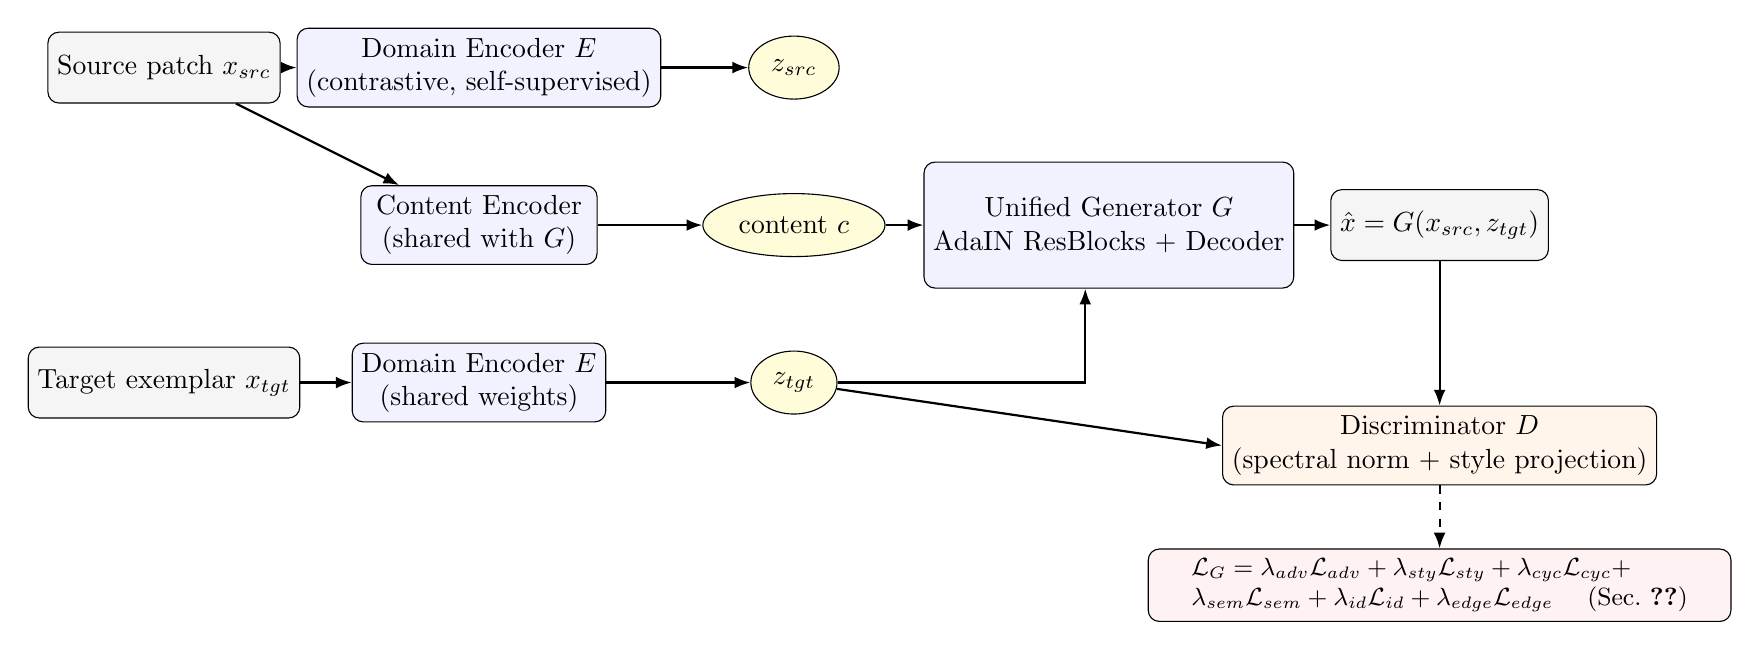
\begin{tikzpicture}[
  node distance=8mm and 10mm,
  box/.style={draw, rounded corners, align=center, minimum height=1.0cm, font=\normalsize, fill=blue!5},
  data/.style={draw, rounded corners, align=center, minimum height=0.9cm, font=\normalsize, fill=gray!8},
  vec/.style={draw, ellipse, align=center, minimum height=0.8cm, font=\normalsize, fill=yellow!15},
  lossbox/.style={draw, rounded corners, align=left, font=\small, fill=red!5},
  arr/.style={-{Latex[length=2mm]}, thick}
]
  \node[data]                              (xsrc) at (0,6)    {Source patch $x_{src}$};
  \node[data]                              (xtgt) at (0,2)    {Target exemplar $x_{tgt}$};

  \node[box, minimum width=3.0cm]          (E1)   at (4.0,6)  {Domain Encoder $E$\\(contrastive, self-supervised)};
  \node[box, minimum width=3.0cm]          (CE)   at (4.0,4)  {Content Encoder\\(shared with $G$)};
  \node[box, minimum width=3.0cm]          (E2)   at (4.0,2)  {Domain Encoder $E$\\(shared weights)};

  \node[vec]                               (zsrc) at (8.0,6)  {$z_{src}$};
  \node[vec]                               (c)    at (8.0,4)  {content $c$};
  \node[vec]                               (ztgt) at (8.0,2)  {$z_{tgt}$};

  \node[box, minimum width=3.2cm, minimum height=1.6cm] (G) at (12.0,4) {Unified Generator $G$\\AdaIN ResBlocks + Decoder};

  \node[data, minimum width=2.6cm]         (xfake) at (16.2,4) {$\hat{x} = G(x_{src}, z_{tgt})$};

  \node[box, fill=orange!8, minimum width=3.0cm] (D) at (16.2,1.2) {Discriminator $D$\\(spectral norm + style projection)};

  \draw[arr] (xsrc) -- (E1);
  \draw[arr] (xsrc) -- (CE);
  \draw[arr] (xtgt) -- (E2);
  \draw[arr] (E1) -- (zsrc);
  \draw[arr] (CE) -- (c);
  \draw[arr] (E2) -- (ztgt);
  \draw[arr] (c) -- (G);
  \draw[arr] (ztgt.east) -| ([xshift=-3mm]G.south);
  \draw[arr] (G) -- (xfake);
  \draw[arr] (xfake) -- (D);
  \draw[arr] (ztgt) -- (D.west);

  \node[lossbox, below=8mm of D, minimum width=7.4cm] (losses) {
    $\mathcal{L}_G = \lambda_{adv}\mathcal{L}_{adv} + \lambda_{sty}\mathcal{L}_{sty} + \lambda_{cyc}\mathcal{L}_{cyc} +$\\
    $\lambda_{sem}\mathcal{L}_{sem} + \lambda_{id}\mathcal{L}_{id} + \lambda_{edge}\mathcal{L}_{edge}$ \quad (Sec.~\ref{sec:objective})
  };
  \draw[arr, dashed] (D.south) -- (losses.north);
\end{tikzpicture}}
\caption{Simplified architecture of the two components reported in this paper: the self-supervised continuous domain encoder $E$ (Objective~1, Sec.~\ref{sec:encoder}) and the unified AdaIN-conditioned generator $G$ with its projection discriminator $D$ (Objective~2, Sec.~\ref{sec:generator}). For clarity, the figure omits two additional forward passes of the source embedding $z_{src}$ through $G$, which are used to compute the cycle-consistency and identity losses of Sec.~\ref{sec:objective}. Components that belong to later objectives of the project (leave-one-pair-out generalization testing and downstream task evaluation) are not shown, because they are outside the scope of this paper.}
\label{fig:architecture}
\end{figure}

Fig.~\ref{fig:architecture} shows the two components covered in this paper. A domain encoder $E$ maps an unlabeled image patch to a continuous style embedding. A content encoder, which is the downsampling path of the generator, extracts a domain-invariant spatial content code. A unified generator $G$ then combines the content of a source patch with the embedding of a target patch to synthesize a translation, which is assessed by a projection discriminator $D$.

\subsection{Self-Supervised Continuous Domain Encoder}
\label{sec:encoder}
The encoder $E_\theta$ receives an $H \times W$ patch with $C$ channels (4 in this implementation: three optical/SAR-derived channels plus one auxiliary channel, see Sec.~\ref{sec:dataset}) and outputs a continuous embedding $z \in \mathbb{R}^{64}$. An input-adapter convolution is followed by three stride-2 convolutional blocks (each Conv--InstanceNorm--LeakyReLU), which progressively reduce the spatial resolution while increasing the channel width. A squeeze-and-excitation (SE) block~\cite{hu2018senet} then recalibrates the channel-wise responses so that the encoder can attend to the most discriminative bands (e.g., near-infrared for vegetation, VV/VH ratio for SAR).

Instead of pooling to a class score, the encoder computes first- and second-order spatial statistics of the final feature map, namely the channel-wise mean $\mu$ and standard deviation $\sigma$. Together, they summarize the radiometric and textural style of the patch independently of its spatial content:
\begin{equation}
\mu_c = \frac{1}{HW}\sum_{i,j} h_{c,i,j}, \qquad
\sigma_c = \sqrt{\frac{1}{HW}\sum_{i,j}(h_{c,i,j}-\mu_c)^2 + \epsilon}
\label{eq:stats}
\end{equation}
where $h$ is the feature map after the SE block. The concatenated statistics $[\mu;\sigma]$ (optionally fused with a projected acquisition-angle feature when angle metadata are available; this option is unused in the sensor-only experiment reported here) pass through a multilayer perceptron projection head and are L2-normalized onto the unit hypersphere:
\begin{equation}
z = \frac{f_\phi([\mu;\sigma])}{\lVert f_\phi([\mu;\sigma]) \rVert_2}, \qquad z \in \mathbb{R}^{64}.
\label{eq:embed}
\end{equation}

The encoder is pretrained without domain labels, using a contrastive pretext task in the style of InfoNCE~\cite{oord2018cpc}. Two independently augmented views ($z_1, z_2$) of the same patch (random flips and 90\textdegree{} rotations) form a positive pair, whereas all other patches in the training batch serve as negatives:
\begin{equation}
\mathcal{L}_{con} = -\frac{1}{2B}\sum_{i=1}^{B}\Big[
\log\frac{e^{\,z_{1,i}\cdot z_{2,i}/\tau}}{\sum_{j} e^{\,z_{1,i}\cdot z_{2,j}/\tau}}
+
\log\frac{e^{\,z_{2,i}\cdot z_{1,i}/\tau}}{\sum_{j} e^{\,z_{2,i}\cdot z_{1,j}/\tau}}
\Big]
\label{eq:infonce}
\end{equation}
where $B$ is the batch size and $\tau$ is a temperature hyperparameter. Since the positive/negative structure comes purely from data augmentation and not from sensor labels, the embedding space is learned without any supervision of domain identity. At inference time, any patch, whether from a domain seen during training or not, can be projected into the same continuous space.

\subsection{Unified Conditional Generator}
\label{sec:generator}
The generator $G_\psi$ receives a source patch $x_{src}$ and a target embedding $z_{tgt}$, which the frozen encoder $E$ produces from a target-domain exemplar, and it synthesizes a translated patch $\hat{x} = G_\psi(x_{src}, z_{tgt})$. One generator instance is shared across all domains, and the target style is determined entirely by $z_{tgt}$. Translation into any domain that the encoder can embed, and not only the domains enumerated at training time, therefore requires neither architectural changes nor additional parameters.

The content path follows an encoder-bottleneck-decoder design in the spirit of StarGAN~v2~\cite{choi2020starganv2}, adapted to be label-free. A content encoder with reflection-padded convolutions and instance normalization downsamples $x_{src}$ into a domain-invariant content code $c = \mathrm{Enc}_c(x_{src})$. This code passes through four residual blocks modulated by Adaptive Instance Normalization (AdaIN)~\cite{huang2017adain}, which injects the target style at every block:
\begin{equation}
\mathrm{AdaIN}(h, z) = \gamma(z)\cdot\frac{h - \mu(h)}{\sigma(h)} + \beta(z)
\label{eq:adain}
\end{equation}
where $\mu(h), \sigma(h)$ are the per-channel instance statistics of the intermediate feature map $h$, and $\gamma(z) = W_\gamma z + b_\gamma$, $\beta(z) = W_\beta z + b_\beta$ are affine parameters regressed from the continuous embedding. The decoder mirrors the encoder with two AdaIN-modulated upsampling stages. It uses bilinear upsampling, instead of nearest-neighbor or transposed-convolution upsampling, to avoid checkerboard artifacts, and it ends with a reflection-padded output convolution with a $\tanh$ activation.

\subsection{Discriminator with Continuous Style Projection}
The discriminator $D_\xi$ is a multi-scale PatchGAN in which spectral normalization~\cite{miyato2018spectral} is applied to every convolutional layer; this stabilizes adversarial training by bounding the Lipschitz constant of each layer. Besides an unconditional real/fake head, $D_\xi$ projects its intermediate features onto the conditioning embedding $z$:
\begin{equation}
D_\xi(x, z) = D_{uncond}(x) + \frac{\langle \phi(x), W_{proj}\,z\rangle}{\sqrt{d}}
\label{eq:disc}
\end{equation}
where $\phi(x)$ is the penultimate feature map of the discriminator, $W_{proj}$ is a learned linear projection of the embedding, and $d$ is the feature dimension. This term penalizes translations whose visual style does not match the conditioning embedding $z$, and it thereby complements the style-reconstruction signal obtained from the encoder (Sec.~\ref{sec:objective}).

\subsection{Composite Training Objective}
\label{sec:objective}
The generator is trained with a weighted sum of six loss terms. Each term targets a specific failure mode observed in unconstrained multi-domain translation.

\emph{Adversarial loss} (least-squares GAN~\cite{mao2017lsgan}), which encourages $\hat{x}$ to be indistinguishable from real target-domain patches under the style-conditioned discriminator:
\begin{align}
\mathcal{L}_D &= \tfrac{1}{2}\mathbb{E}\big[(D_\xi(x_{tgt}, z_{tgt}) - 1)^2\big] + \tfrac{1}{2}\mathbb{E}\big[D_\xi(\hat{x}, z_{tgt})^2\big] \\
\mathcal{L}_{adv} &= \mathbb{E}\big[(D_\xi(\hat{x}, z_{tgt}) - 1)^2\big]
\label{eq:adv}
\end{align}

\emph{Style-reconstruction loss}, which requires that the target style can be measured in the output by re-encoding it:
\begin{equation}
\mathcal{L}_{sty} = \mathbb{E}\,\lVert E(\hat{x}) - z_{tgt} \rVert_1
\label{eq:sty}
\end{equation}

\emph{Cycle-consistency loss}~\cite{zhu2017cyclegan}, which translates $\hat{x}$ back toward the source style and requires the original patch to be recovered, thereby discouraging mode collapse across domains:
\begin{equation}
\mathcal{L}_{cyc} = \mathbb{E}\,\lVert G(\hat{x}, z_{src}) - x_{src} \rVert_1
\label{eq:cyc}
\end{equation}

\emph{Semantic-preservation loss}, which penalizes drift of the domain-invariant content code between the source and the translation, so that the geospatial layout (parcel boundaries, roads) is not altered by the style change:
\begin{equation}
\mathcal{L}_{sem} = \mathbb{E}\,\lVert \mathrm{Enc}_c(\hat{x}) - \mathrm{Enc}_c(x_{src}) \rVert_1
\label{eq:sem}
\end{equation}

\emph{Identity loss}, which requires that conditioning the generator on the source's own style leaves the patch unchanged:
\begin{equation}
\mathcal{L}_{id} = \mathbb{E}\,\lVert G(x_{src}, z_{src}) - x_{src} \rVert_1
\label{eq:id}
\end{equation}

\emph{Edge-preservation loss}, which compares the Sobel gradient magnitudes of $\hat{x}$ and $x_{src}$ in order to keep agricultural parcel boundaries and road edges sharp:
\begin{equation}
\mathcal{L}_{edge} = \mathbb{E}\,\lVert \nabla_{Sobel}(\hat{x}) - \nabla_{Sobel}(x_{src}) \rVert_1
\label{eq:edge}
\end{equation}

The total generator objective is
\begin{align}
\mathcal{L}_G ={}& \lambda_{adv}\mathcal{L}_{adv} + \lambda_{sty}\mathcal{L}_{sty} + \lambda_{cyc}\mathcal{L}_{cyc} \notag \\
& + \lambda_{sem}\mathcal{L}_{sem} + \lambda_{id}\mathcal{L}_{id} + \lambda_{edge}\mathcal{L}_{edge}
\label{eq:total}
\end{align}
with the weights listed in Table~\ref{tab:hyperparams}. In addition, the framework defines a geometric (SSIM-style) preservation loss $\mathcal{L}_{geo}$, which is activated when the source or the target domain is an off-nadir viewing-angle domain. The PASTIS-HD experiment reported in Sec.~\ref{sec:results} uses only sensor domains, so $\mathcal{L}_{geo}$ is inactive ($\lambda_{geo}\mathcal{L}_{geo}=0$) for the results presented here.

\section{Dataset and Preprocessing}
\label{sec:dataset}
The experiments use patches derived from PASTIS-HD~\cite{garnot2021panoptic,astruc2024omnisat}, a real and publicly released benchmark of $2{,}433$ co-registered agricultural-parcel locations across metropolitan France. Each location is available as a Sentinel-2 optical time series, a Sentinel-1 SAR time series, and, in the HD extension, a very-high-resolution SPOT~6/7 image. A conversion pipeline in the accompanying codebase matches patches across modalities by their shared patch identifier and exports one $128\times128$, 4-channel tensor per modality and location. For Sentinel-2, only the Red, Green, Blue, and near-infrared bands of a single temporal acquisition are kept. The SPOT~6/7 imagery is resized from its native $1280\times1280$ resolution to $128\times128$ and supplemented with a synthetic near-infrared proxy channel. The VV and VH polarizations of Sentinel-1 SAR are extended with a derived ratio channel and an average channel, and are normalized from decibel units. All modalities are scaled to $[-1,1]$. Of the up to $2{,}433$ available locations, this experiment converts $1{,}500$ per domain, a number limited by the patch cap of the conversion pipeline (Table~\ref{tab:dataset}). The converted patches are the first $1{,}500$ in identifier order and originate from three Sentinel-2 tiles. An 80/20 split by identifier order yields $1{,}200$ training patches and $300$ held-out patches per domain. As a consequence, all held-out patches belong to a single tile (T31TFM) that is only marginally represented in the training data, so the held-out evaluation is largely a test on a different region. The modalities are co-registered but not simultaneous: the first Sentinel-1 acquisition follows the first Sentinel-2 acquisition by 11~days at the median, and the SPOT imagery dates from 2019, whereas the Sentinel data begin in September 2018. After conversion, the SAR difference channel is saturated at $+1$ for 97.9\% of its values. Training-split patches are augmented on the fly with random horizontal and vertical flips, random 90\textdegree{} rotations, and small per-channel Gaussian radiometric noise ($\sigma \sim \mathcal{U}[0, 0.01]$).

\begin{table}[t]
\centering
\caption{Converted PASTIS-HD patches used in this study.}
\label{tab:dataset}
\begin{tabular}{@{}lccc@{}}
\toprule
\textbf{Domain} & \textbf{Modality} & \textbf{Channels} & \textbf{Patches} \\
\midrule
Sentinel-2       & Multispectral optical (R,G,B,NIR) & 4 & 1{,}500 \\
SPOT 6/7         & VHR optical (+NIR proxy)          & 4 & 1{,}500 \\
Sentinel-1 SAR   & C-band radar (VV, VH, ratio, avg) & 4 & 1{,}500 \\
\bottomrule
\end{tabular}
\end{table}

\section{Experimental Setup}
\label{sec:setup}
The framework is implemented in Python~3.13 with PyTorch~$\geq$2.4; NumPy, SciPy, Pillow, Matplotlib, and PyYAML are used for data handling, preprocessing, and visualization. A single command-line entry point orchestrates training: it first runs domain-encoder pretraining and then trains the generator and discriminator jointly. All training and evaluation were run on the CPU of a laptop (Intel Core i7-9750H, 6 cores, 7.8~GB RAM, Windows~11) with a CPU-only PyTorch build. The channel width of the generator and discriminator was deliberately kept narrow (base width 32) so that training remains tractable at this compute scale, and not in order to match a specific reported baseline configuration. Table~\ref{tab:hyperparams} lists the hyperparameters used for the results in Sec.~\ref{sec:results}.

\begin{table}[t]
\centering
\caption{Training hyperparameters.}
\label{tab:hyperparams}
\begin{tabular}{@{}ll@{}}
\toprule
\textbf{Stage 1 -- Domain Encoder} & \textbf{Value} \\
\midrule
Embedding dimension $d$            & 64 \\
Optimizer                          & AdamW \\
Learning rate                      & $5\times10^{-4}$ \\
Weight decay                       & $1\times10^{-4}$ \\
Contrastive temperature $\tau$     & 0.07 \\
Epochs                             & 10 \\
\midrule
\textbf{Stage 2 -- Generator / Discriminator} & \textbf{Value} \\
\midrule
Base channel width                 & 32 \\
Residual blocks                    & 4 \\
Optimizer ($G$, $D$)               & Adam ($\beta_1{=}0.5$, $\beta_2{=}0.999$) \\
Learning rate ($G$, $D$)           & $3\times10^{-4}$ \\
LR schedule                        & Cosine annealing, $\eta_{min}{=}10^{-5}$ \\
Gradient clipping (max norm)       & 1.0 \\
Epochs                             & 12 \\
Batch size                         & 8 \\
$\lambda_{adv},\lambda_{sty},\lambda_{id}$ & 1.0 each \\
$\lambda_{sem}$, $\lambda_{edge}$  & 2.0 each \\
$\lambda_{cyc}$                    & 10.0 \\
\bottomrule
\end{tabular}
\end{table}

\section{Results and Discussion}
\label{sec:results}
All results were measured on the 300 held-out patches per domain with a fixed protocol, and each is a single measurement of one trained model. The style of a target domain is defined as the L2-normalized mean of the embeddings of its 1{,}200 training patches (the domain \emph{centroid}); domain labels and co-registered patches are used only for evaluation. Image metrics are computed on images rescaled to $[0,1]$ against the co-registered real target patch, and two reference baselines are included: the untranslated source patch (``Copy'') and a constant image equal to the mean of the target domain (``Const.'').

\subsection{Domain encoder (Objective~1)}
Table~\ref{tab:enc} summarizes the results for the encoder. It solves its contrastive task on held-out patches (loss 0.24, against 2.08 for an uninformative embedding; 88.2\% top-1 retrieval of the second view among 900 patches), and its embeddings are distributed continuously over the hypersphere and do not form three tight clusters. However, they describe the sensor only moderately well: the nearest centroid assigns 65.8\% of the held-out patches to the correct sensor, against 33.3\% by chance; the sensors overlap (silhouette coefficient 0.11); and the effective dimensionality is about four. Retrieval of the co-registered patch from another sensor is at chance level, which indicates that the embedding does not carry scene content shared across sensors. A likely explanation, which was not tested, is that instance discrimination rewards distinguishing individual patches and includes no term that groups the patches of one sensor; the proximity-based positive pairs foreseen in the project plan were not used.

\begin{table}[t]
\centering
\caption{Domain encoder evaluated on 300 held-out patches per domain (S2: Sentinel-2).}
\label{tab:enc}
\begin{tabular}{@{}lc@{}}
\toprule
\textbf{Measurement} & \textbf{Result} \\
\midrule
Held-out InfoNCE loss (batch 8; chance 2.08)        & 0.24 \\
Top-1 instance retrieval among 900 patches          & 88.2\% \\
Nearest-centroid domain accuracy (chance 33.3\%)    & 65.8\% \\
\quad recall S2 / SPOT / SAR                        & 62.7 / 74.3 / 60.3\% \\
5-nearest-neighbor domain accuracy                  & 63.7\% \\
Cosine similarity within / between domains          & 0.32 / 0.04 \\
Silhouette coefficient (cosine distance)            & 0.11 \\
Participation ratio (of 64 dimensions)              & 3.85 \\
Same-location retrieval across sensors, top-1       & 0.3\% (chance 0.3\%) \\
\bottomrule
\end{tabular}
\end{table}

\subsection{Conditional generator (Objective~2)}
\begin{figure}[t]
\centering
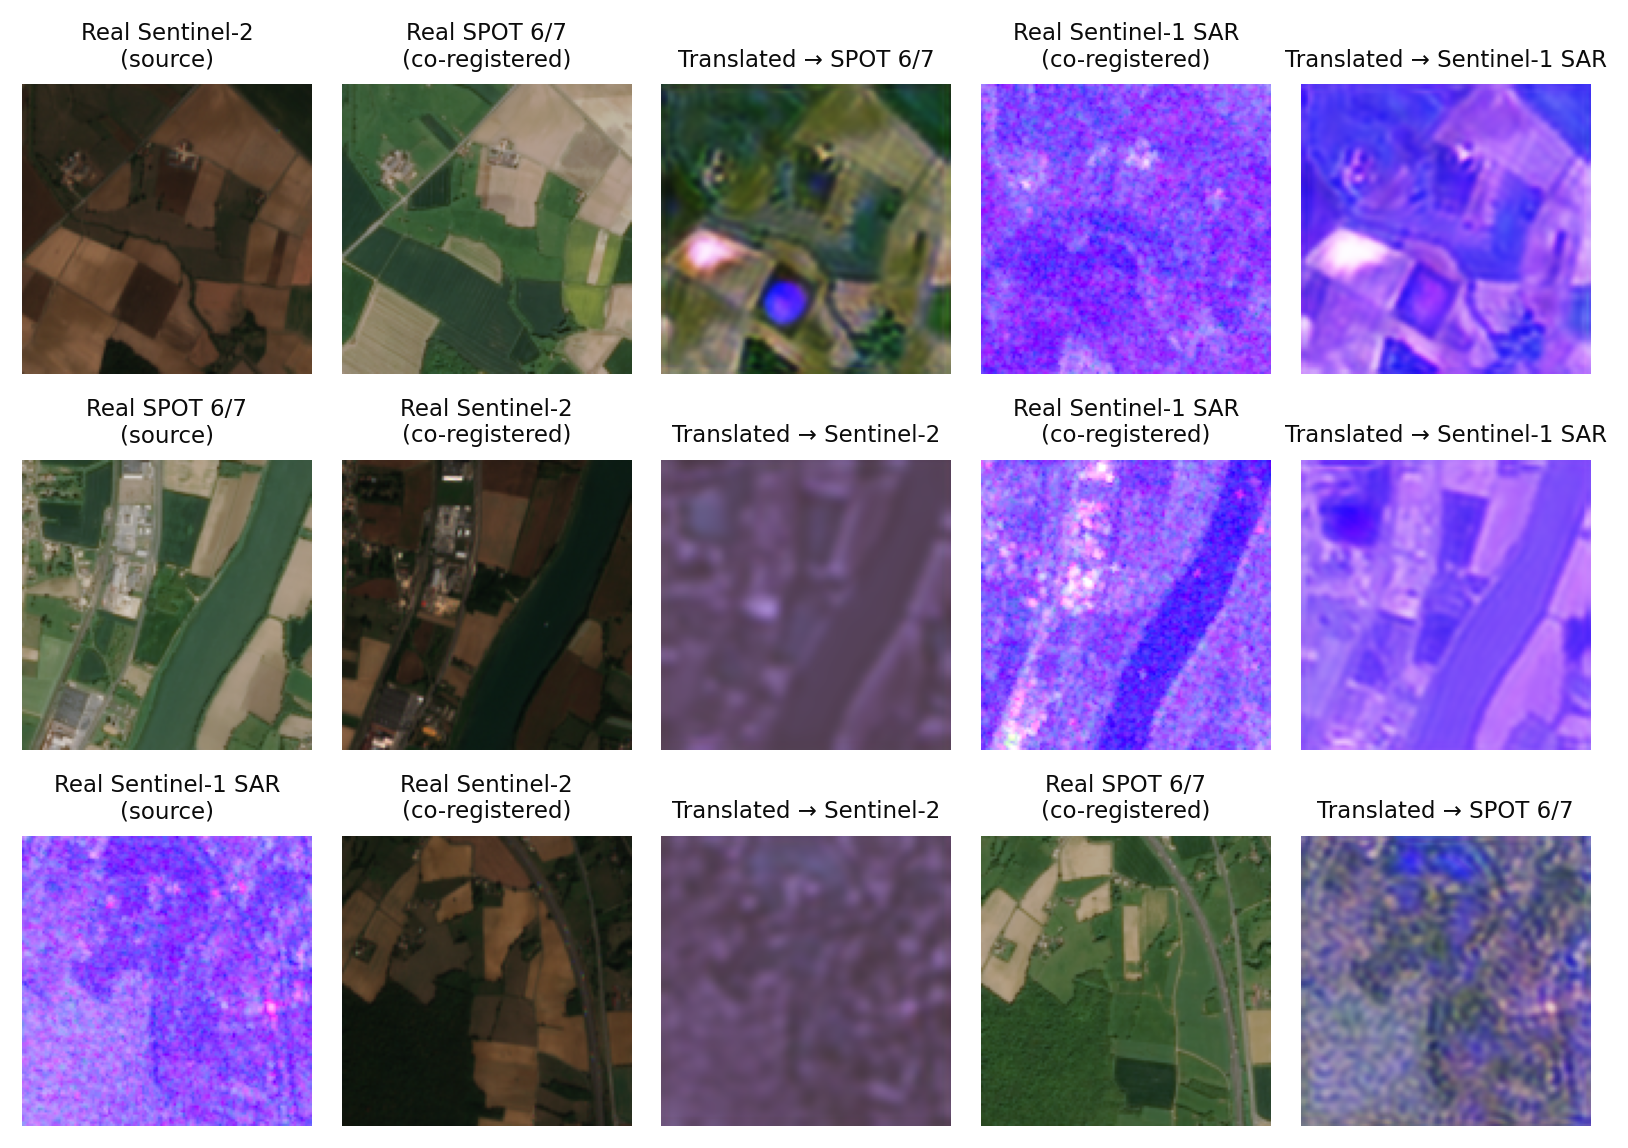
\includegraphics[width=\textwidth]{figures/fig_paired_translation.png}
\caption{Translations of one held-out patch per source domain (first column of each row) into the two other domains, shown next to the real co-registered patch of each target domain. The style is the centroid embedding of the target domain, and the patches were selected with a fixed random seed before inspection. Sentinel-1 patches are displayed with VV, VH, and the saturated difference channel as the red, green, and blue channels, respectively.}
\label{fig:paired}
\end{figure}

\begin{table}[t]
\centering
\caption{Translation into each target domain on held-out patches. PSNR (dB) against the co-registered real target patch is given for the translation, for the copied source (Copy), and for a constant target-mean image (Const.). Style is the share of outputs that the encoder assigns to the target domain, and Edge is the edge-map correlation with the source.}
\label{tab:gen}
\footnotesize
\setlength{\tabcolsep}{3.5pt}
\begin{tabular}{@{}lccccc@{}}
\toprule
\textbf{Pair} & \textbf{Transl.} & \textbf{Copy} & \textbf{Const.} & \textbf{Style} & \textbf{Edge} \\
\midrule
S2 $\rightarrow$ SPOT   & 14.6 & 13.1 & 17.2 & 57\% & 0.82 \\
S2 $\rightarrow$ SAR    & 14.6 & 5.7 & 20.5 & 18\% & 0.87 \\
SPOT $\rightarrow$ S2   & 13.5 & 13.1 & 17.8 & 29\% & 0.71 \\
SPOT $\rightarrow$ SAR  & 16.8 & 7.4 & 20.5 & 80\% & 0.82 \\
SAR $\rightarrow$ S2    & 13.3 & 5.7 & 17.8 & 12\% & 0.94 \\
SAR $\rightarrow$ SPOT  & 13.0 & 7.4 & 17.2 & 45\% & 0.92 \\
\bottomrule
\end{tabular}
\end{table}

Fig.~\ref{fig:paired} and Table~\ref{tab:gen} summarize the results for the generator. \emph{Structure is preserved:} the edge-map correlation between the source and the output ranges from 0.71 to 0.94, which is higher than the 0.61 to 0.70 observed between real patches of different sensors, and parcels, the river, and the road remain recognizable in the figure. \emph{The style vector is used:} with the correct target style, the PSNR is higher than with the style of the third domain for five of the six pairs (by 3.3 to 7.6~dB), and the translation is better than copying the source for all six pairs, most strongly for the pairs that involve SAR. \emph{Target radiometry is not reproduced:} for all six pairs, a constant image equal to the target-domain mean agrees better with the real target patch than the translation does (by 2.6 to 5.9~dB). In addition, the encoder assigns the outputs to the target domain in only 12\% to 80\% of the cases. Translations into Sentinel-2 appear as a blurred purple-gray haze whose channel means are identical for all three sources (within 0.001) and much brighter than those of real Sentinel-2 patches (by 0.59 in the blue channel on a $[-1,1]$ scale). The identity mapping of Sentinel-2 is also poorly reproduced (13.7~dB, compared with 20.3~dB for SPOT and 24.3~dB for SAR), which makes Sentinel-2 the weak point of the generator both as a source and as a target. Differences in acquisition date between the modalities limit the achievable pixel agreement, but they do not explain why the translation is worse than a constant image.

\emph{Continuity of the style space} was examined by interpolating between two domain centroids, $z(\alpha)=(1-\alpha)\bar z_a+\alpha\bar z_b$, renormalized to unit length, for 300 source patches. For the two pairs that involve SAR, the output changes smoothly and almost linearly (linearity ratio 0.91 and 0.96; monotone for 96\% and 100\% of the patches). For Sentinel-2 and SPOT, the change is about half as large, is concentrated in the first step from $\alpha=0$ to $\alpha=0.25$, and is monotone for only 41\% of the patches. The generator has 1.59~M parameters and the encoder 0.89~M, and one translation takes about 84~ms per patch on the CPU. Fig.~\ref{fig:interp} illustrates this interpolation for one held-out SPOT~6/7 source patch.

\begin{figure}[t]
\centering
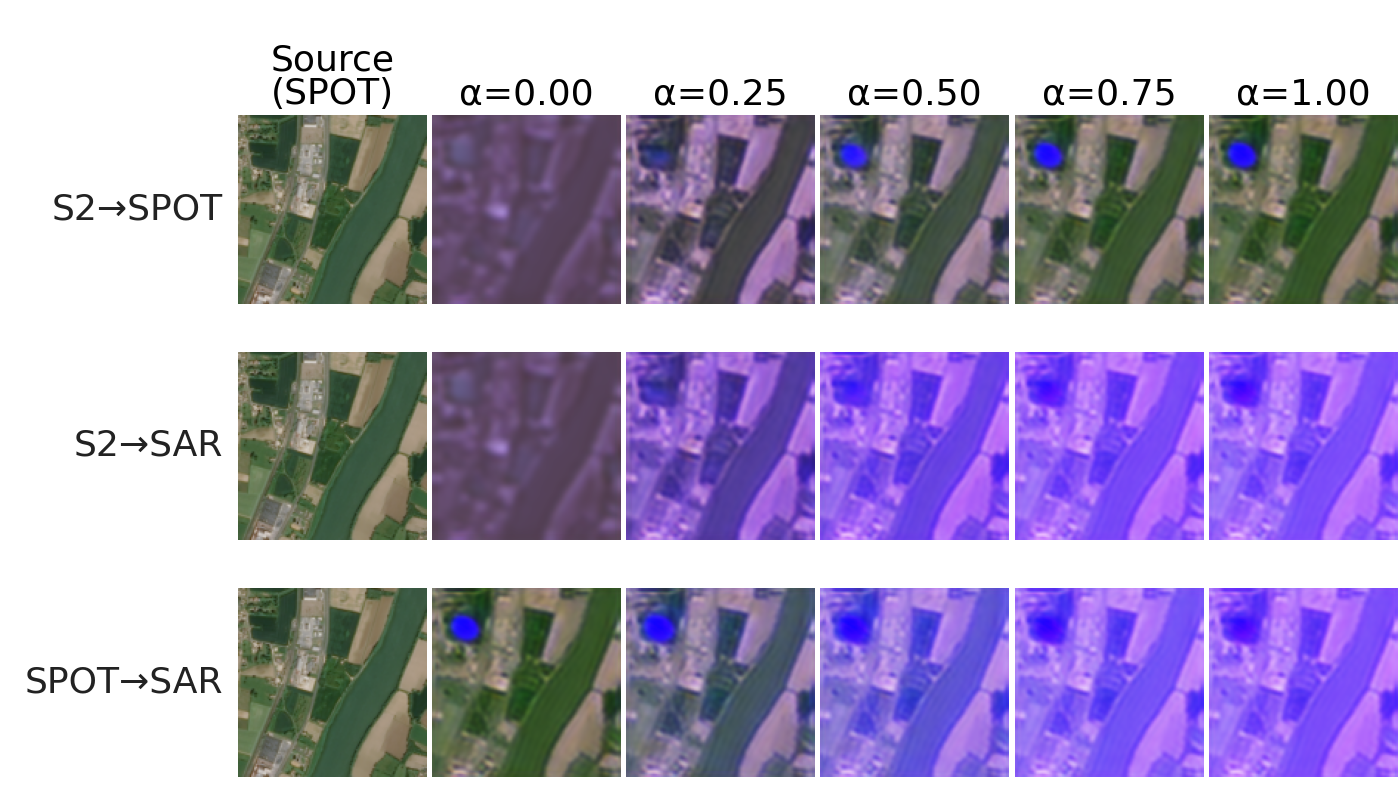
\includegraphics[width=0.85\textwidth]{figures/fig_interp_compact.png}
\caption{Interpolation of the style vector between two domain centroids, $z(\alpha)=(1-\alpha)\bar z_a+\alpha\bar z_b$, renormalized to unit length, applied to one held-out SPOT~6/7 source patch (first column). Each row corresponds to a domain pair $a \rightarrow b$, and $\alpha$ runs from the style of $a$ ($\alpha=0$) to the style of $b$ ($\alpha=1$). The patch was selected with a fixed random seed before inspection.}
\label{fig:interp}
\end{figure}

\section{Comparative Analysis}
Table~\ref{tab:gap} in Sec.~\ref{sec:gap} has already placed the proposed encoder-generator pair alongside the closest prior methods with respect to the properties that motivate this work. In the implementation, the design goals listed in Table~\ref{tab:gap} are met at the architectural level: training uses no domain labels, one generator serves all ordered pairs of three domains, and the domain code is a continuous 64-dimensional embedding. The quality of the results, however, cannot be compared with the cited methods, because none of them was trained on the same data and their published figures come from other datasets and tasks. Accordingly, no claim is made that the approach outperforms SS(DA)$^2$, StarGAN~v2, or the other methods.

\section{Limitations}
\label{sec:limitations}
Several limitations should be kept in mind when interpreting the results in Sec.~\ref{sec:results}. First, the held-out patches come from a single Sentinel-2 tile, whereas the training set is dominated by two other tiles; the results therefore combine model quality with a region shift, and in particular the domain centroids come from mostly different regions than the patches to which they are applied. Second, the modalities are not simultaneous, which limits pixel-level agreement with the co-registered reference, and the preprocessing introduces artifacts (a saturated SAR channel and a synthetic fourth SPOT channel). Third, each model was trained only once, with a short schedule (10 encoder and 12 generator epochs), a narrow network (base width 32), and a CPU-only laptop (Sec.~\ref{sec:setup}). The training loops are not seeded, the run-to-run variation is unknown, no ablation of the six generator losses was run, and no other translation method was trained on the same data for comparison. Fourth, PSNR and SSIM measure agreement with a co-registered image and not realism, and the style-transfer success rate is judged by the same encoder that conditions the generator, so it is only as reliable as that encoder. Fifth, only three sensor domains, one geographic setting, and $1{,}500$ of the $2{,}433$ locations are used; the larger MSC-France corpus foreseen for encoder pretraining was not used, and the angle-domain conditioning implemented in the framework was not exercised. Finally, generalization to unseen sensor pairs and downstream accuracy (Objectives~3--4) were not evaluated.

\section{Conclusion and Future Work}
This paper presented the first two components of a self-supervised, multi-domain adaptation framework for satellite imagery. The first is a contrastive domain encoder that learns continuous, label-free embeddings of sensor style from unlabeled multi-sensor patches. The second is a unified AdaIN-conditioned generator that uses this embedding, in place of the discrete domain labels required by prior multi-domain translators, to translate the content of a source patch into an arbitrary target style. Implemented and trained on real PASTIS-HD imagery across Sentinel-2, SPOT~6/7, and Sentinel-1 SAR, the framework meets its design goals at the architectural level: no domain labels, one model for all ordered domain pairs, and a continuous domain code. The measured quality is limited, however. The encoder identifies the sensor only moderately (65.8\% against 33.3\% by chance), and the generator preserves scene structure and uses the style vector but does not reproduce the radiometry of the target sensor, while translations into Sentinel-2 fail.

Building directly on these findings, future work will (i) replace the augmented-view positives of the encoder with sensor-aware positive pairs based on spatial and temporal proximity, and pretrain on the larger MSC-France corpus; (ii) correct the data issues identified here by using all PASTIS-HD patches with a tile-stratified split, temporally matched acquisitions, and a non-saturating SAR channel; (iii) train wider networks for longer on a GPU, with seeded and logged runs, loss ablations, and baselines trained on the same data; and (iv) carry out the leave-one-domain-pair-out and zero-shot (SpaceNet~6) generalization evaluation, together with the downstream crop-classification and segmentation evaluation, which constitute Objectives~3 and~4 of the broader project.

\bibliographystyle{splncs04}
\bibliography{references}

\end{document}
